% Copyright 2004 by Till Tantau <tantau@users.sourceforge.net>.
%
% In principle, this file can be redistributed and/or modified under
% the terms of the GNU Public License, version 2.
%
% However, this file is supposed to be a template to be modified
% for your own needs. For this reason, if you use this file as a
% template and not specifically distribute it as part of a another
% package/program, I grant the extra permission to freely copy and
% modify this file as you see fit and even to delete this copyright
% notice. 

\documentclass{beamer}
\usepackage[utf8x]{inputenc}            % Acentos, ñ, etc.
\usepackage{graphicx}                   % Gráficos
\usepackage[spanish]{babel}             % Macros en español
\usepackage{float}
\setbeamertemplate{navigation symbols}{}
% There are many different themes available for Beamer. A comprehensive
% list with examples is given here:
% http://deic.uab.es/~iblanes/beamer_gallery/index_by_theme.html
% You can uncomment the themes below if you would like to use a different
% one:
%\usetheme{AnnArbor}
%\usetheme{Antibes}
%\usetheme{Bergen}
%\usetheme{Berkeley}
%\usetheme{Berlin}
%\usetheme{Boadilla}
%\usetheme{boxes}
%\usetheme{CambridgeUS}
%\usetheme{Copenhagen}
%\usetheme{Darmstadt}
%\usetheme{default}
%\usetheme{Frankfurt}
%\usetheme{Goettingen}
%\usetheme{Hannover}
%\usetheme{Ilmenau}
%\usetheme{JuanLesPins}
%\usetheme{Luebeck}
\usetheme{Madrid}
%\usetheme{Malmoe}
%\usetheme{Marburg}
%\usetheme{Montpellier}
%\usetheme{PaloAlto}
%\usetheme{Pittsburgh}
%\usetheme{Rochester}
%\usetheme{Singapore}
%\usetheme{Szeged}
%\usetheme{Warsaw}
\setbeamersize{text margin left=5pt, text margin right=5pt}
\title{¿Qué ves cuando lo ves?}

% A subtitle is optional and this may be deleted
\subtitle{Cómo funciona el lobulo relacionador conceptual}

\author{G. Fernández \and I. Linari \and C. Bonomi}
% - Give the names in the same order as the appear in the paper.
% - Use the \inst{?} command only if the authors have different
%   affiliation.

\institute[UBA] % (optional, but mostly needed)
{
  \inst{1}%
  Departmento de Computación\\
  Universidad de Buenos Aires
  \and
  \inst{2}%
  Department of Theoretical Philosophy\\
  University of Elsewhere}
% - Use the \inst command only if there are several affiliations.
% - Keep it simple, no one is interested in your street address.

\date{INCC, 2016}
% - Either use conference name or its abbreviation.
% - Not really informative to the audience, more for people (including
%   yourself) who are reading the slides online

\subject{Theoretical Computer Science}
% This is only inserted into the PDF information catalog. Can be left
% out. 

% If you have a file called "university-logo-filename.xxx", where xxx
% is a graphic format that can be processed by latex or pdflatex,
% resp., then you can add a logo as follows:

% \pgfdeclareimage[height=0.5cm]{university-logo}{university-logo-filename}
% \logo{\pgfuseimage{university-logo}}

% Delete this, if you do not want the table of contents to pop up at
% the beginning of each subsection:
\AtBeginSubsection[]
{
  \begin{frame}<beamer>{Índice}
    \tableofcontents[currentsection,currentsubsection]
  \end{frame}
}

% Let's get started
\begin{document}

\begin{frame}
  \titlepage
\end{frame}

\begin{frame}{Índice}
  \tableofcontents
  % You might wish to add the option [pausesections]
\end{frame}

% Section and subsections will appear in the presentation overview
% and table of contents.
\section{Introducción}

\subsection{Idea}

\begin{frame}{Motivación}{El origen de este trabajo}
  \begin{itemize}
  \item {
La idea fue ver en qué pensamos cuando vemos un logo. Si nos remite a aquello a lo que el logo referencia o si lo vemoscomo una imagen sin significado. 
  }
  \item {

Por ejemplo: Si ven al logo de coca cola los remite a la gaseosa o solo ven un circulo rojo con letras?.
  }
\begin{figure}[h]
 \centering
  \begin{minipage}[c]{1\textwidth}
	\centering	
	
\includegraphics[scale=0.16]{img/cocacola.jpg}
       % \caption{Experimento}
  \end{minipage}
\end{figure}




   % Nos preguntamos qué tan bien hacen su trabajo los logos de marcas. Las personas cuando los ven identifican Conceptos, Colores, formas, o no les significan nada especifico? 



 
  \end{itemize}
\end{frame}

\begin{frame}{Hipótesis}{La respuesta a todas las preguntas}
  \begin{itemize}
  \item {

Creemos que la gente asocia mayormente por concepto. Es decir, que por mas que un logo no haga referencia explicita a su concepto, las personas pensamos inconscientemente en aquello que el logo representa. 


  }

 
  \end{itemize}
\end{frame}

\subsection{Experimento}

% You can reveal the parts of a slide one at a time
% with the \pause command:
\begin{frame}{Experimento}

\begin{itemize}
\item{Sets: 
	\begin{enumerate}
	\item {Set 1: \\
	Definimos diferentes trials. Cada uno de estos esta compuesto por un logo target y luego 4 logos distintos relacionados con el targuet de acuerdo a 3 categorias: Forma/Letra, Concepto, Color. Además agregamos un cuarto logo al que llamamos Ruido, el cual consideramos que no se relaciona con el target de ninguna manera. A estos cuatro logos los llamamos choices.
    \pause % The slide will pause after showing the first item
  }
	\item {Set 2: \\
Trials Random, en los cuales se toman como target y como choices logos al azar. 
	}
\end{enumerate} 
}
 \pause 
\item {
	Cada participante dado el logo target debe seleccionar según su criterio de asociación, uno de los 4 choices.
  }
    \pause % The slide will pause 
\item {Los trials aparecen intercalados.  
}



\end{itemize}



  
  % or you can use the \uncover command to reveal general
  % content (not just \items):
%  \item<5-> {
%    Fifth item. \uncover<6->{Extra text in the fifth item.}
%  }

\end{frame}

\begin{frame}
\begin{figure}[h]
 \centering
  \begin{minipage}[c]{1\textwidth}
	\centering	
	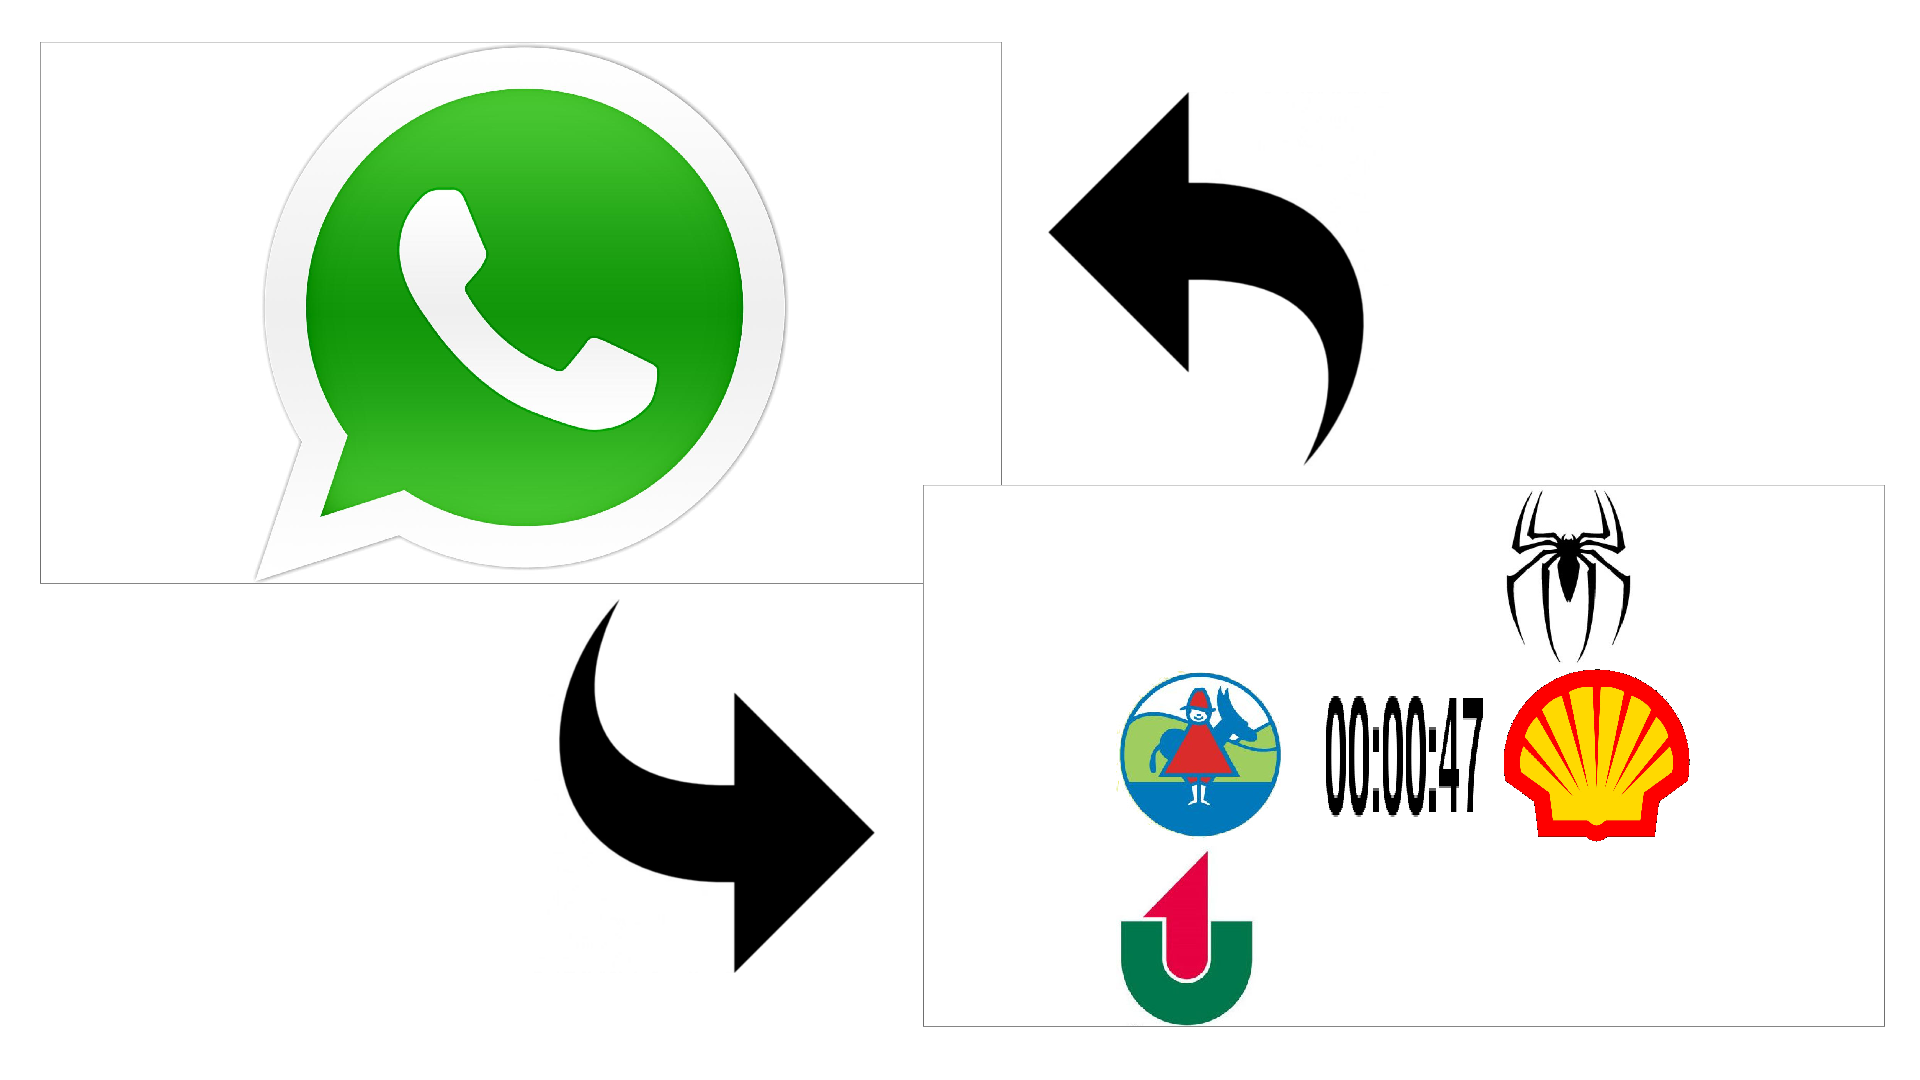
\includegraphics[scale=0.16]{exp.png}
        \caption{Experimento}
  \end{minipage}
\end{figure}
\end{frame}


\subsection{Definiciones}

\begin{frame}{Métricas}
\begin{block}{Índice de Relacion en un trial}
IR = 1/tiempo de respuesta. 
\end{block}

\begin{block}{Indice de relacion de un usuario respecto a una clase.}
$IR\_uxc$ = $\sum IR$ de los trials de ese usuario en los que eligió la clase.
\end{block}

\begin{block}{Índice de relación de un choice respecto a un target.}
$IR\_cxt$ = $\sum IR$ de los trials con el target t en los que se eligió el choice c.
\end{block}

\begin{block}{Índice de relación de un logo respecto a otro logo.}
$IR\_l1xl2$ = $\sum IR$ de los trials con con target l1 en los que se eligió a l2.
\end{block}

%\begin{example}
%Here is an example of an example block.
%\end{example}
\end{frame}

\section{Resultados}

\subsection{Usuarios}


\begin{frame}

\begin{figure}[h]
 \centering
  \begin{minipage}[c]{1\textwidth}
	\centering	
	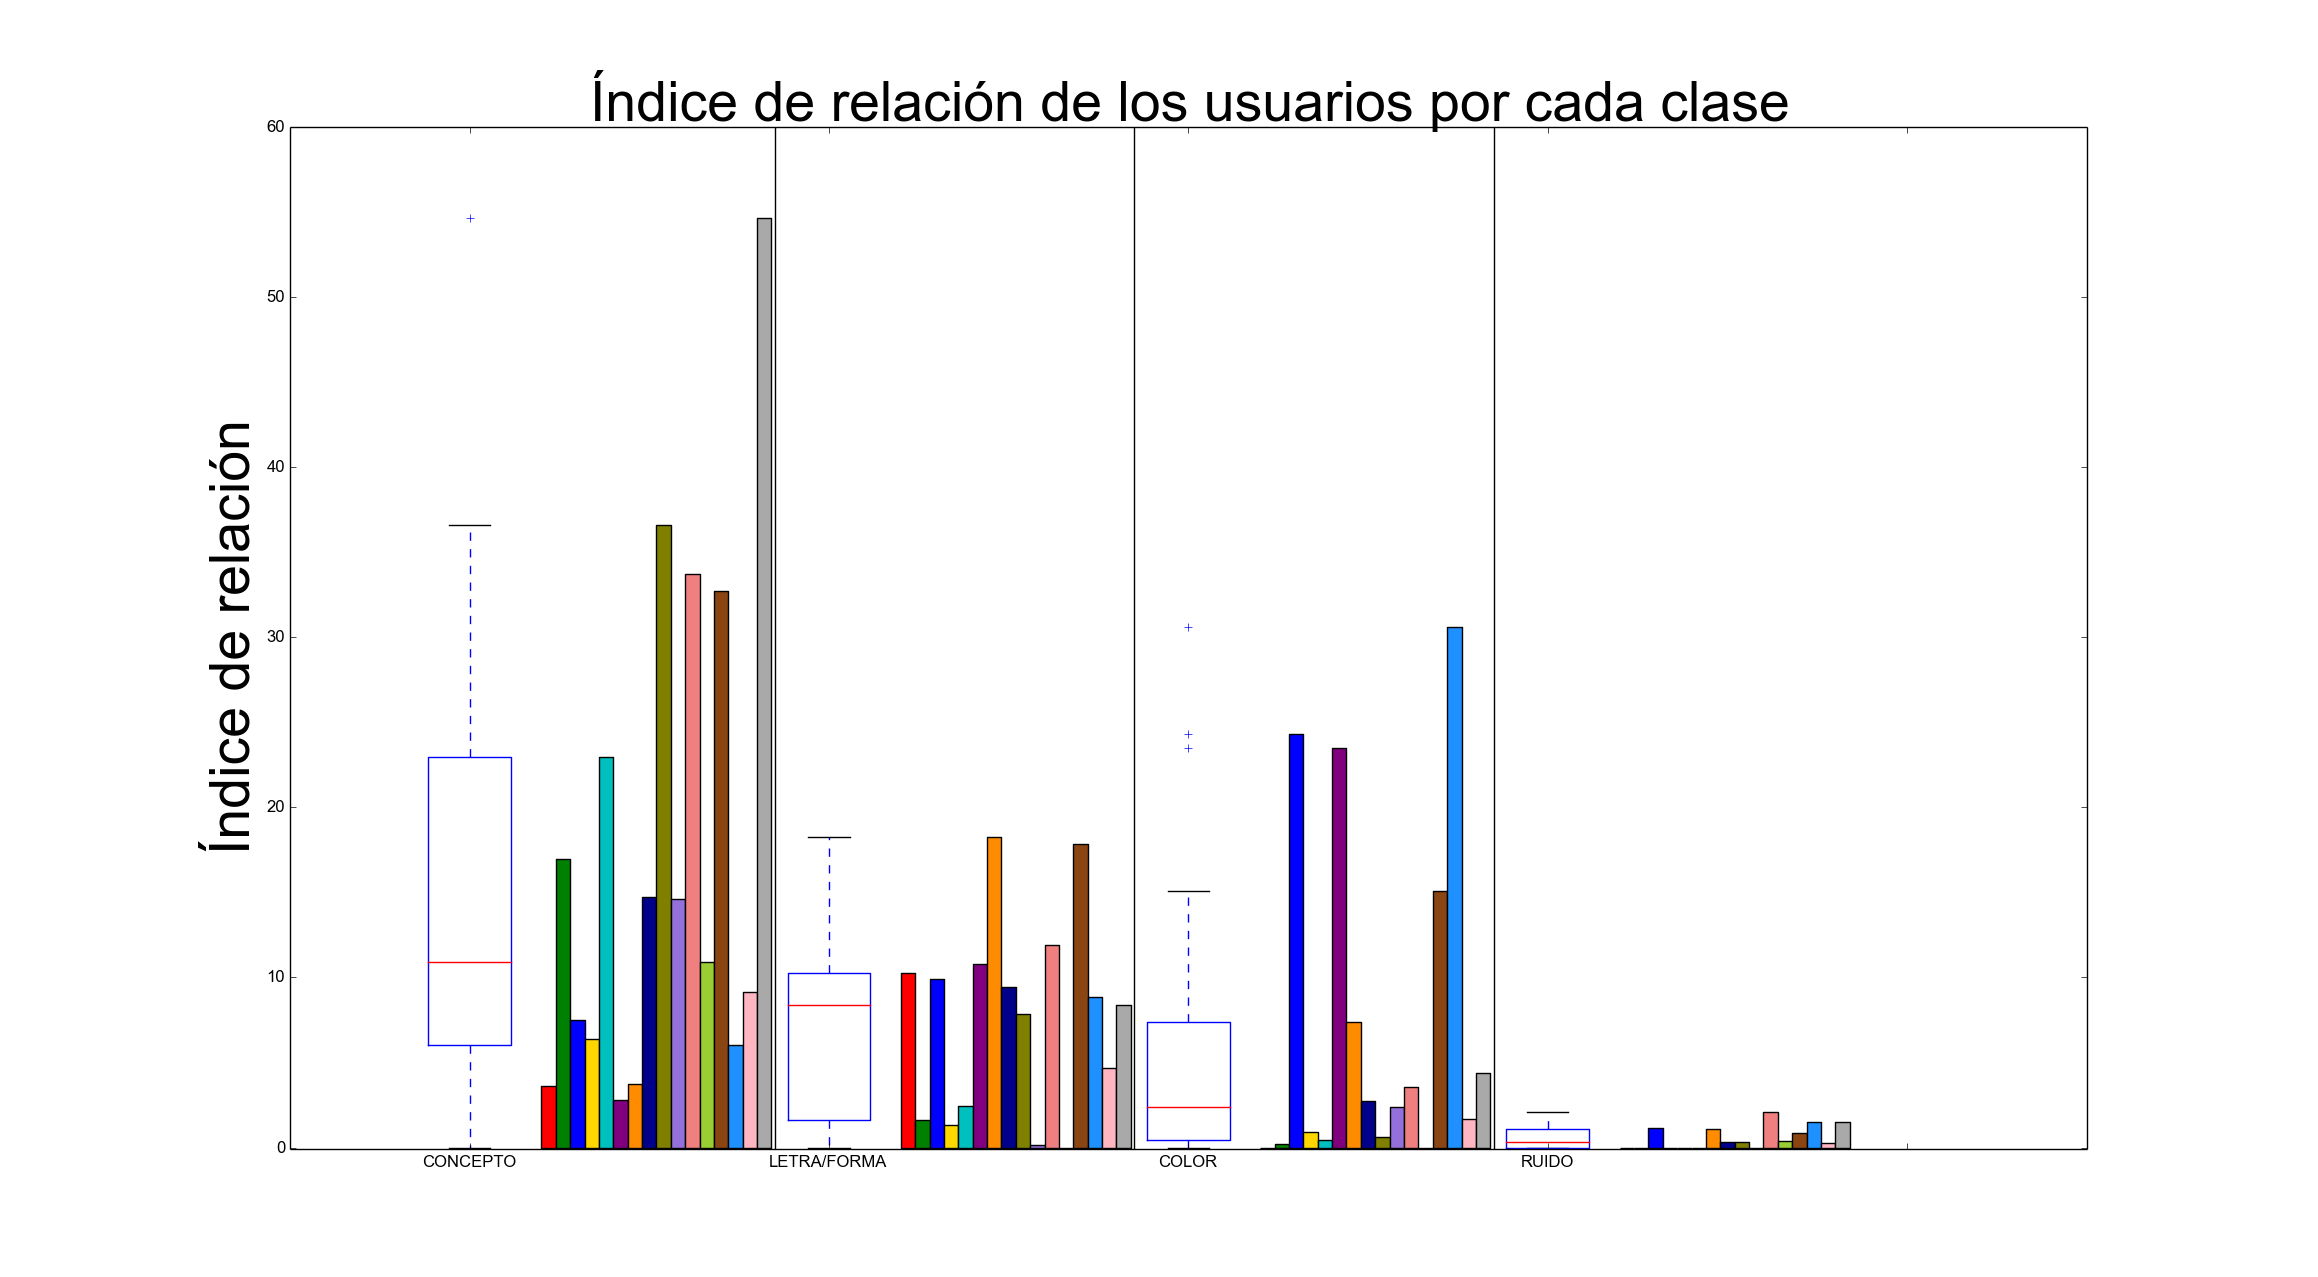
\includegraphics[scale=0.23]{ir_uxc.png}
  \end{minipage}
\end{figure}

\end{frame}
\begin{frame}

\begin{figure}[h]
 \centering
  \begin{minipage}[c]{1\textwidth}
	\centering	
	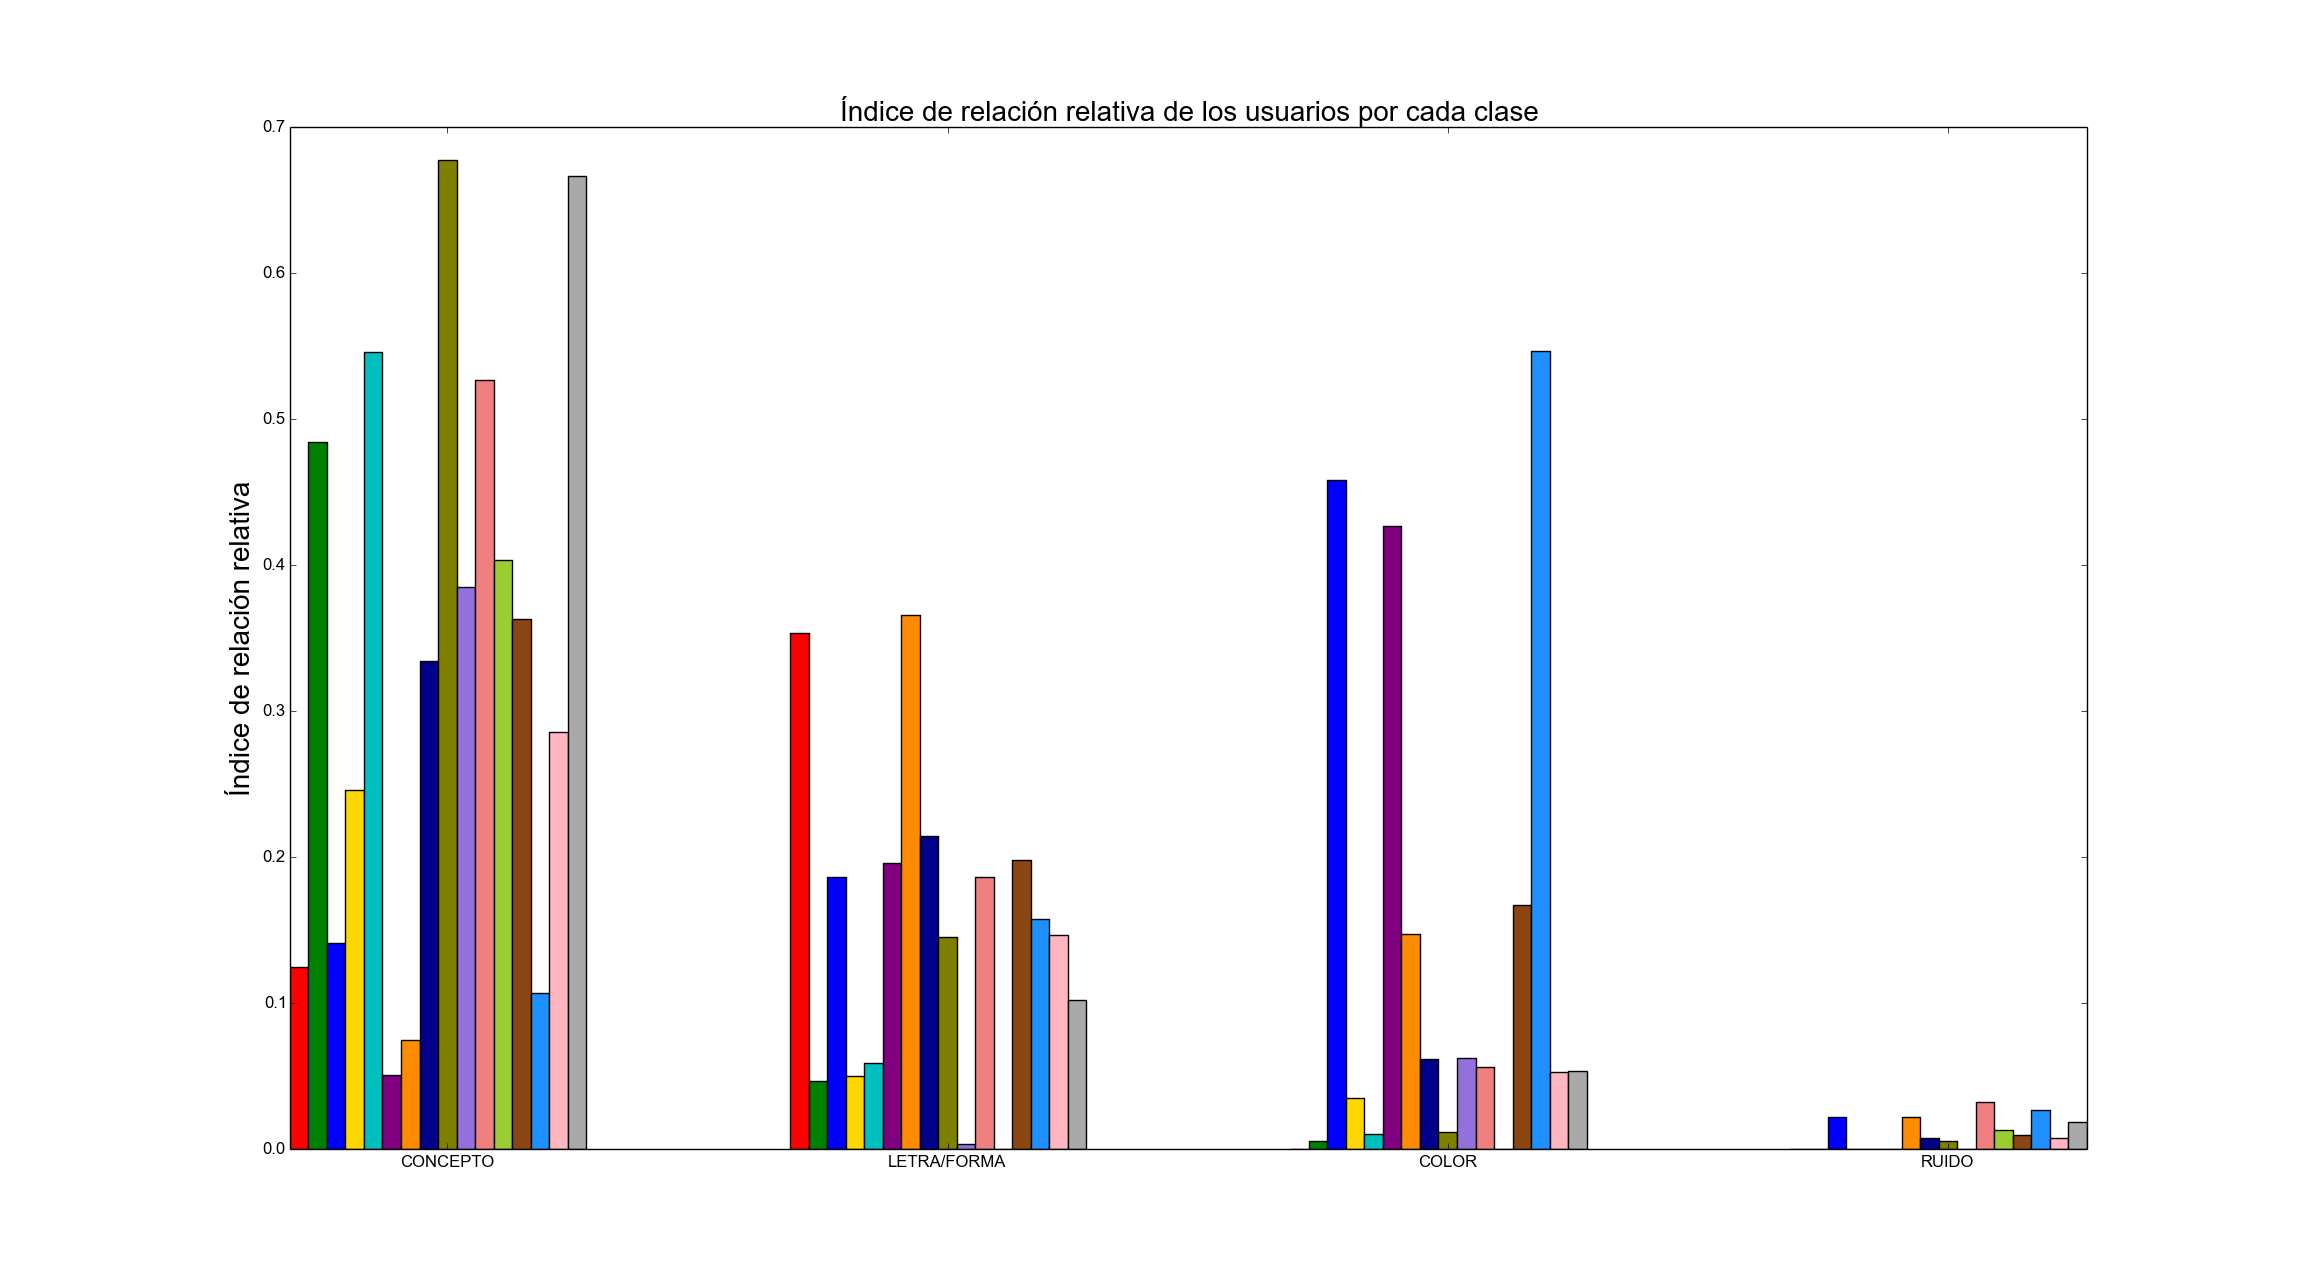
\includegraphics[scale=0.23]{irr_uxc.png}
  \end{minipage}
\end{figure}

\end{frame}

\begin{frame}
\begin{figure}[h]
 \centering
  \begin{minipage}[c]{1\textwidth}
	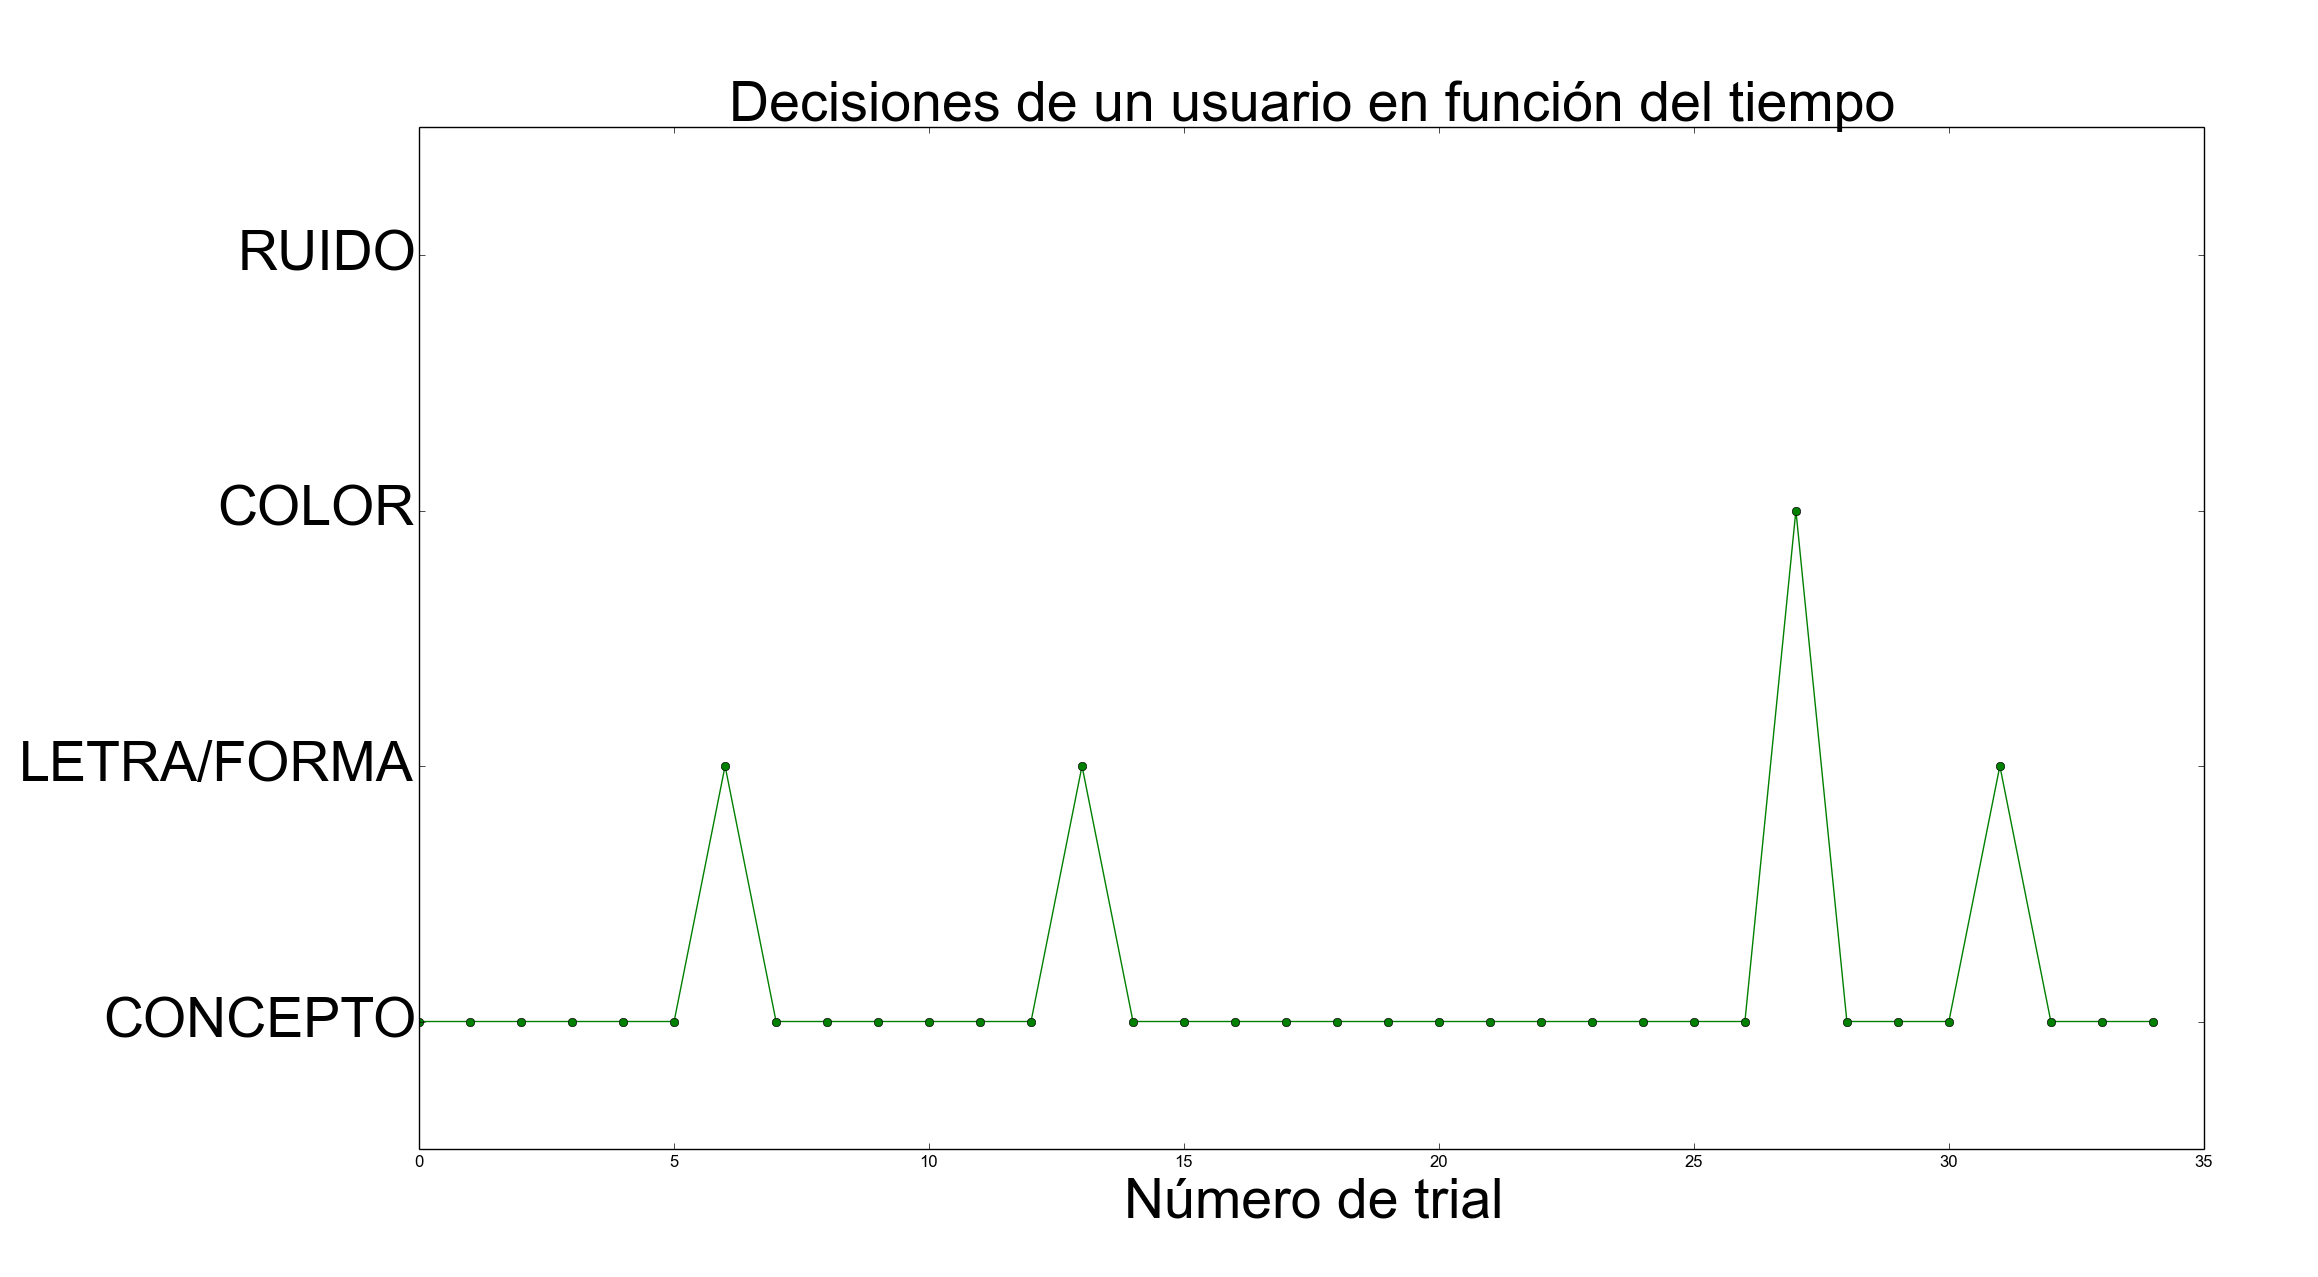
\includegraphics[scale=0.108]{user2.png}
	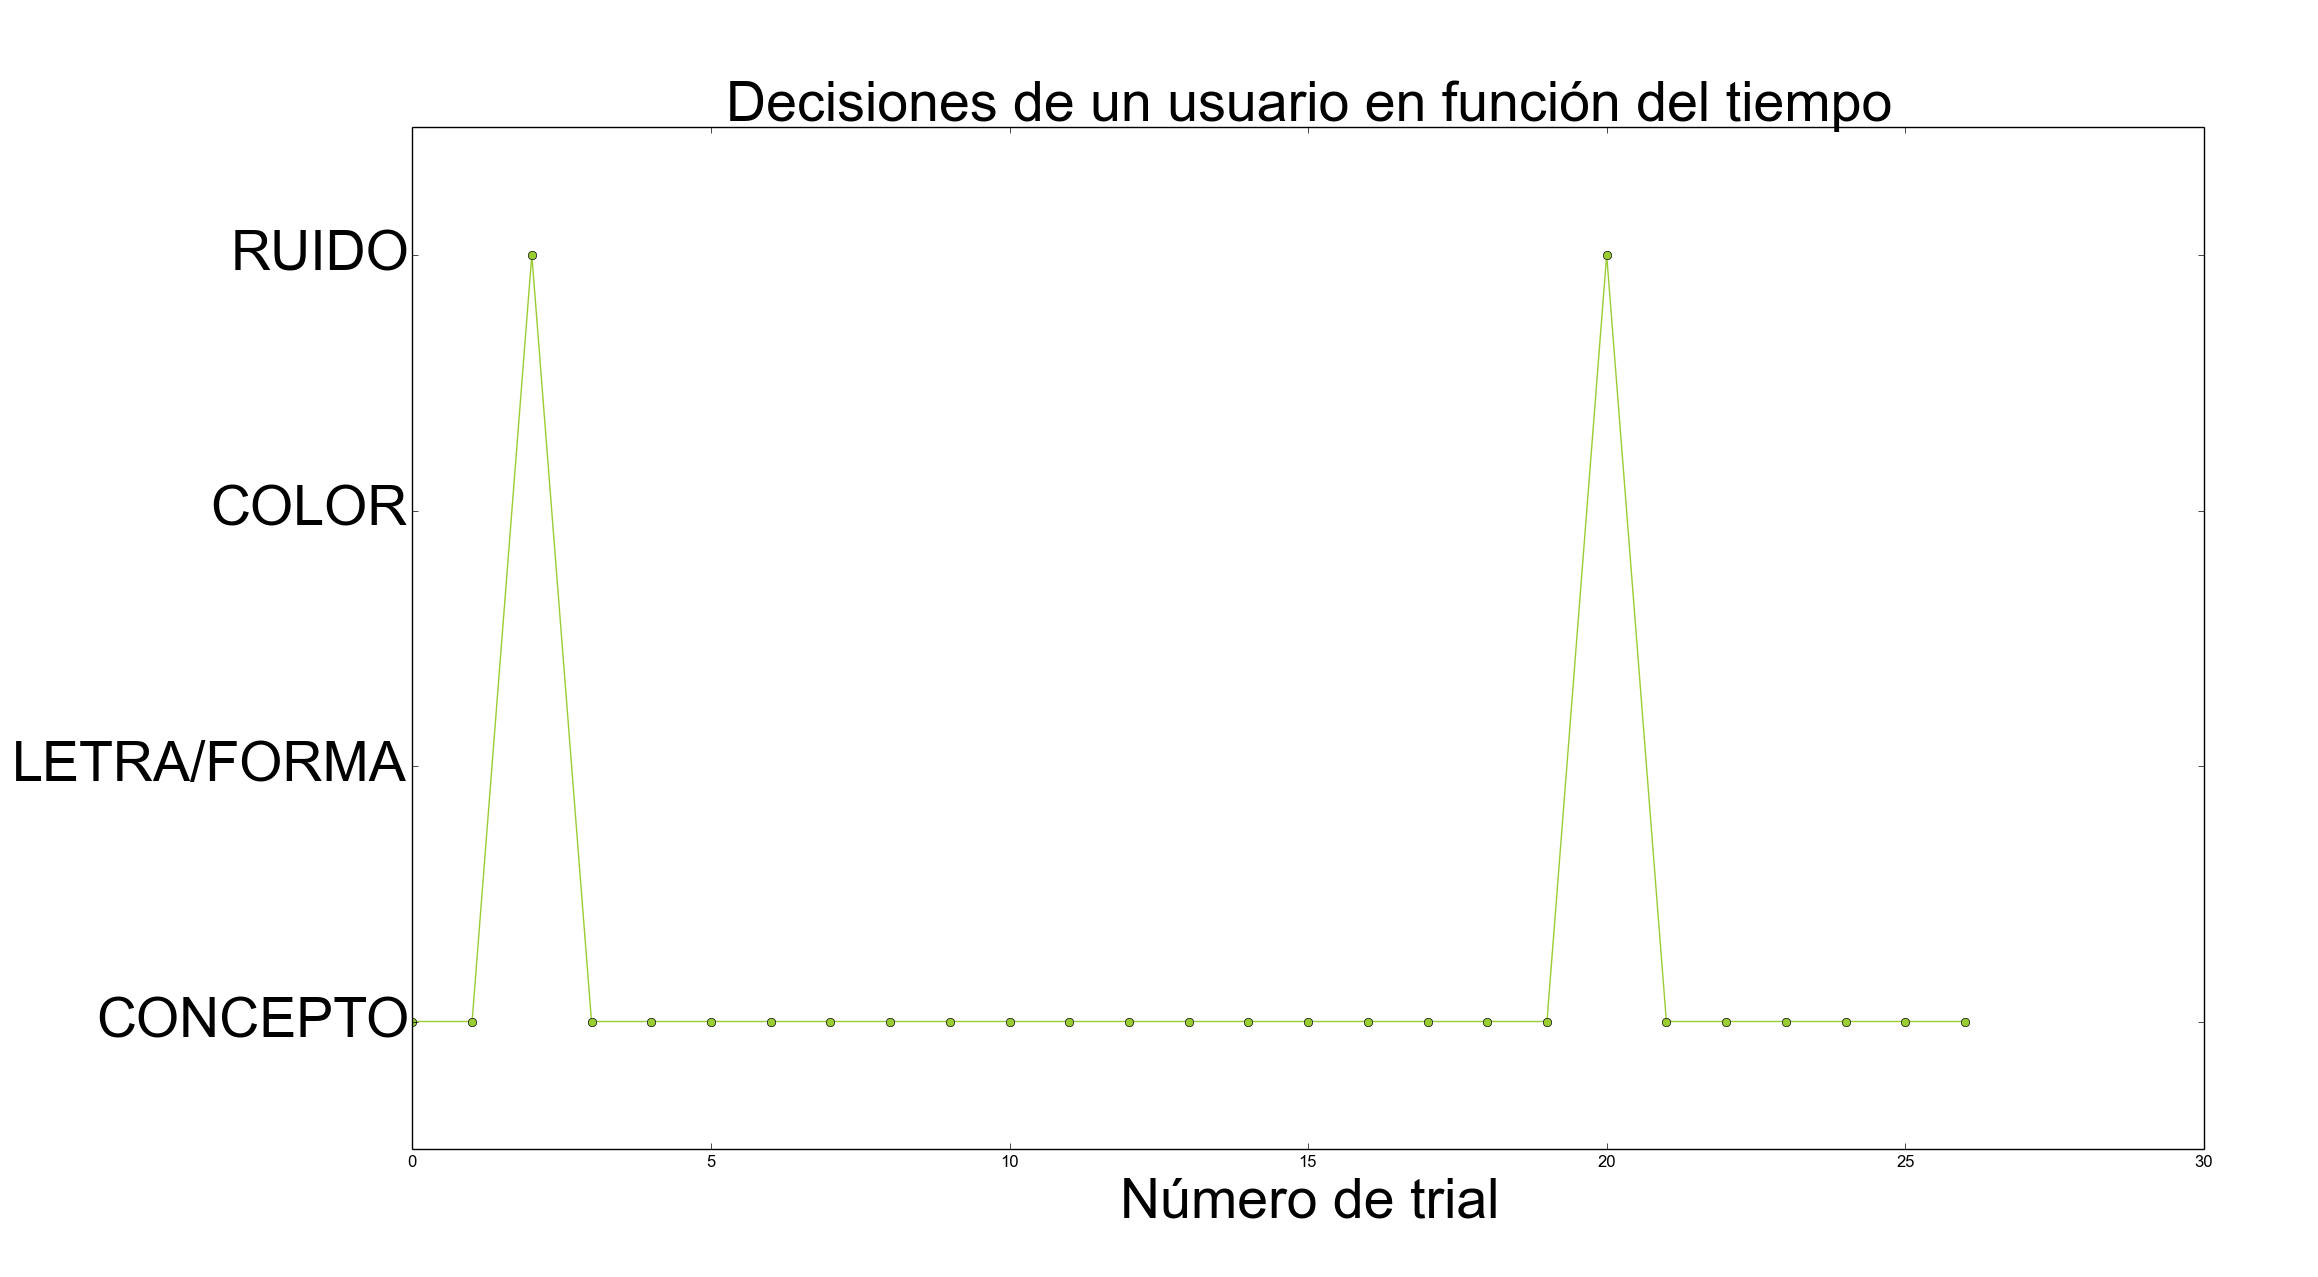
\includegraphics[scale=0.108]{user12.png}
  \end{minipage}
  \begin{minipage}[c]{1\textwidth}
	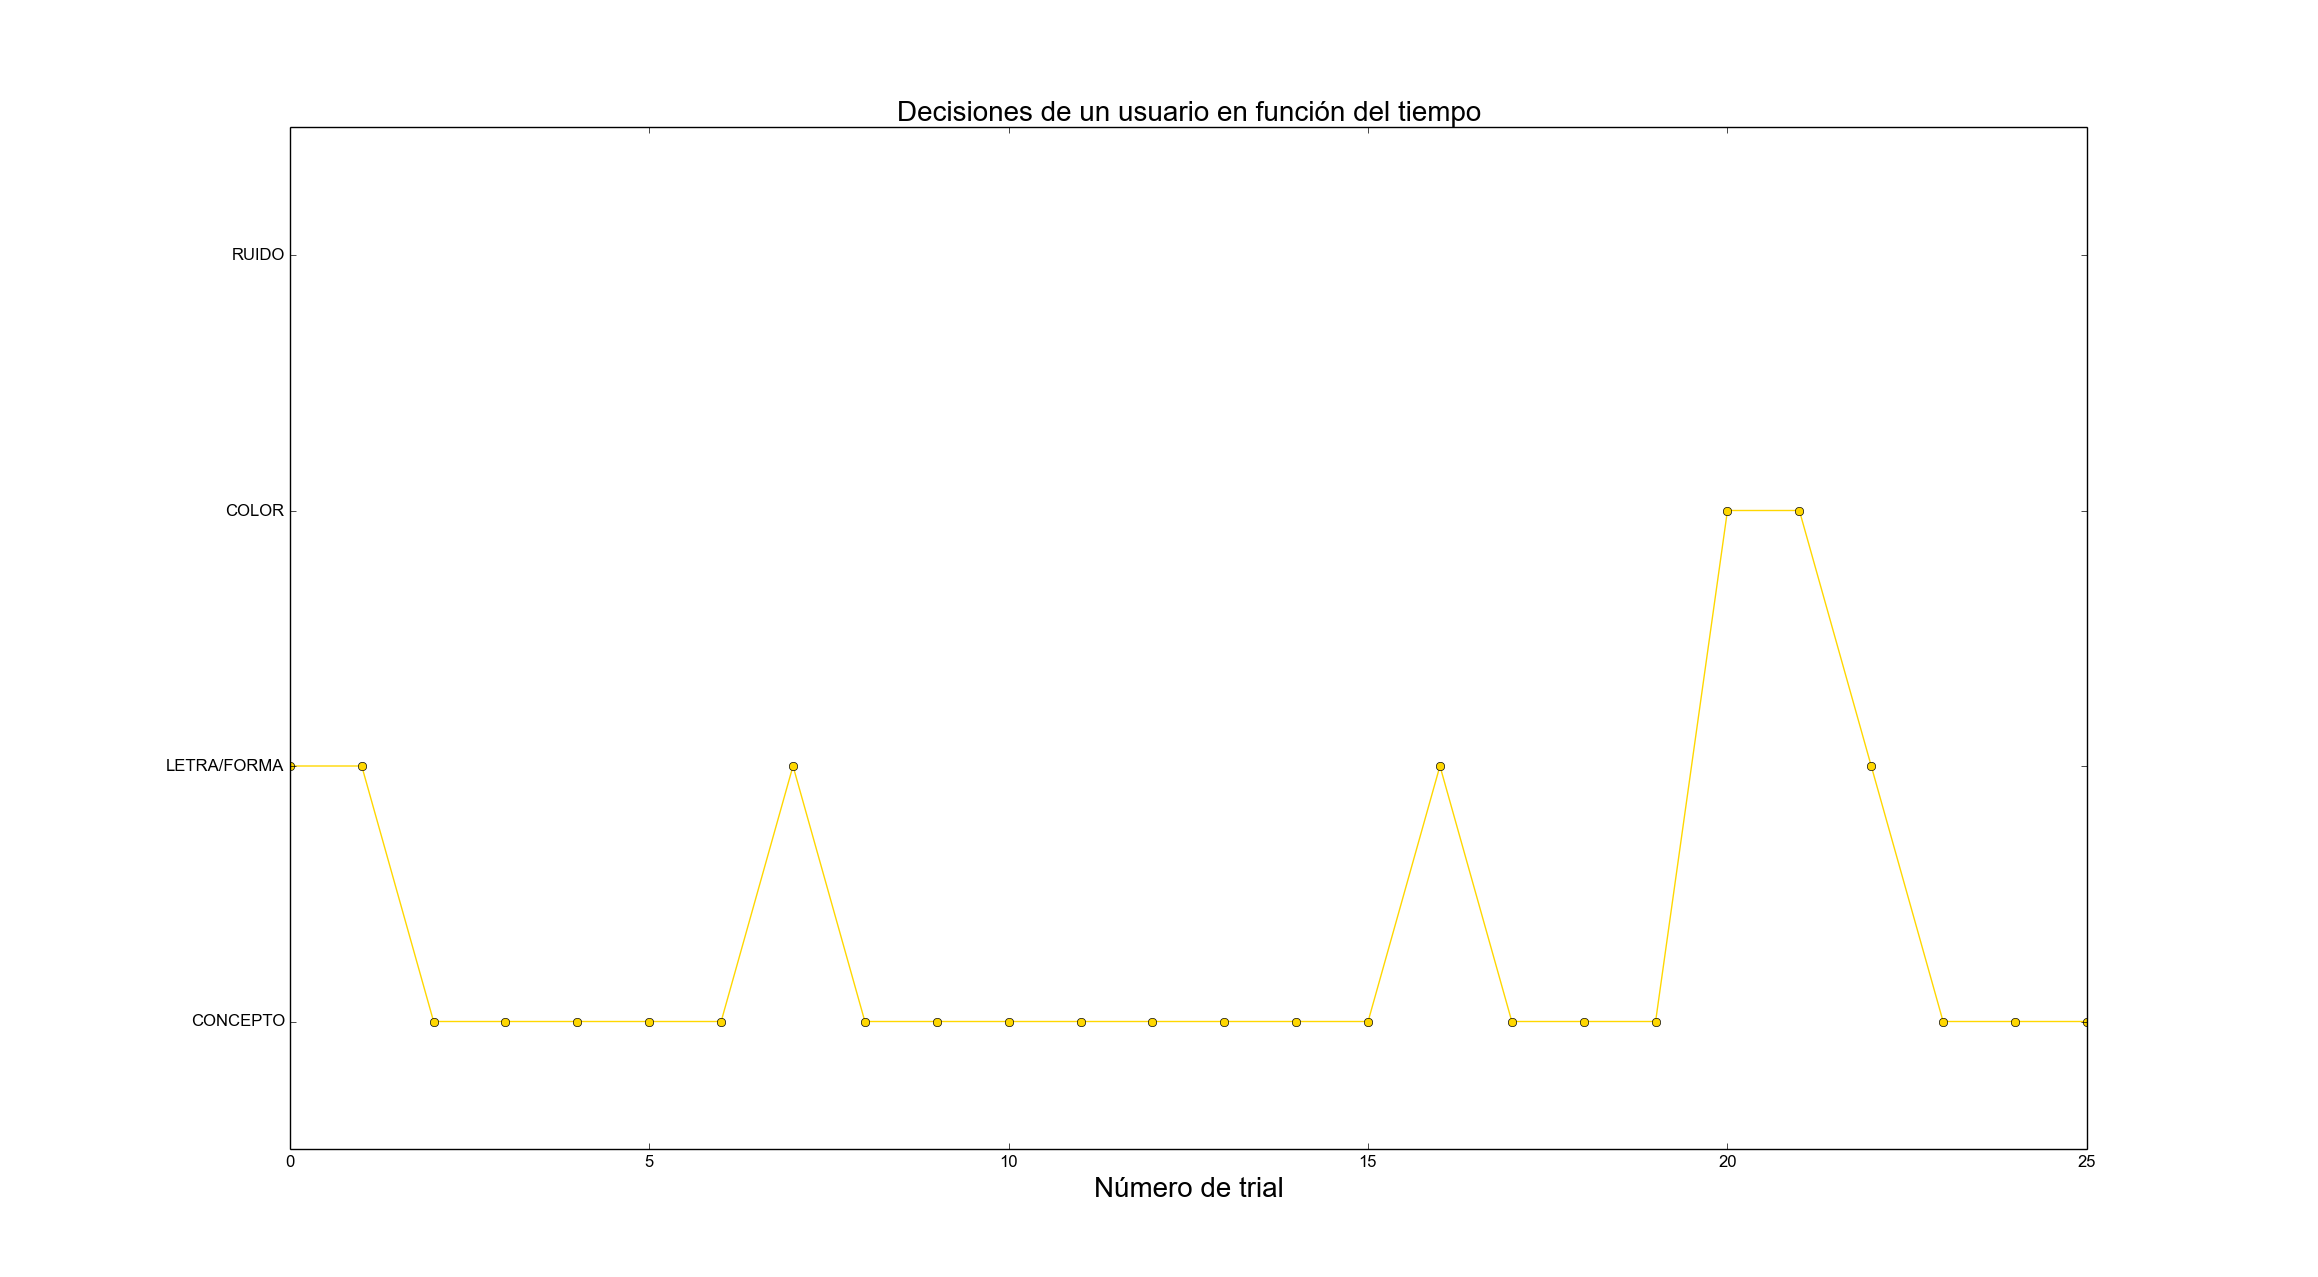
\includegraphics[scale=0.108]{user4.png}
	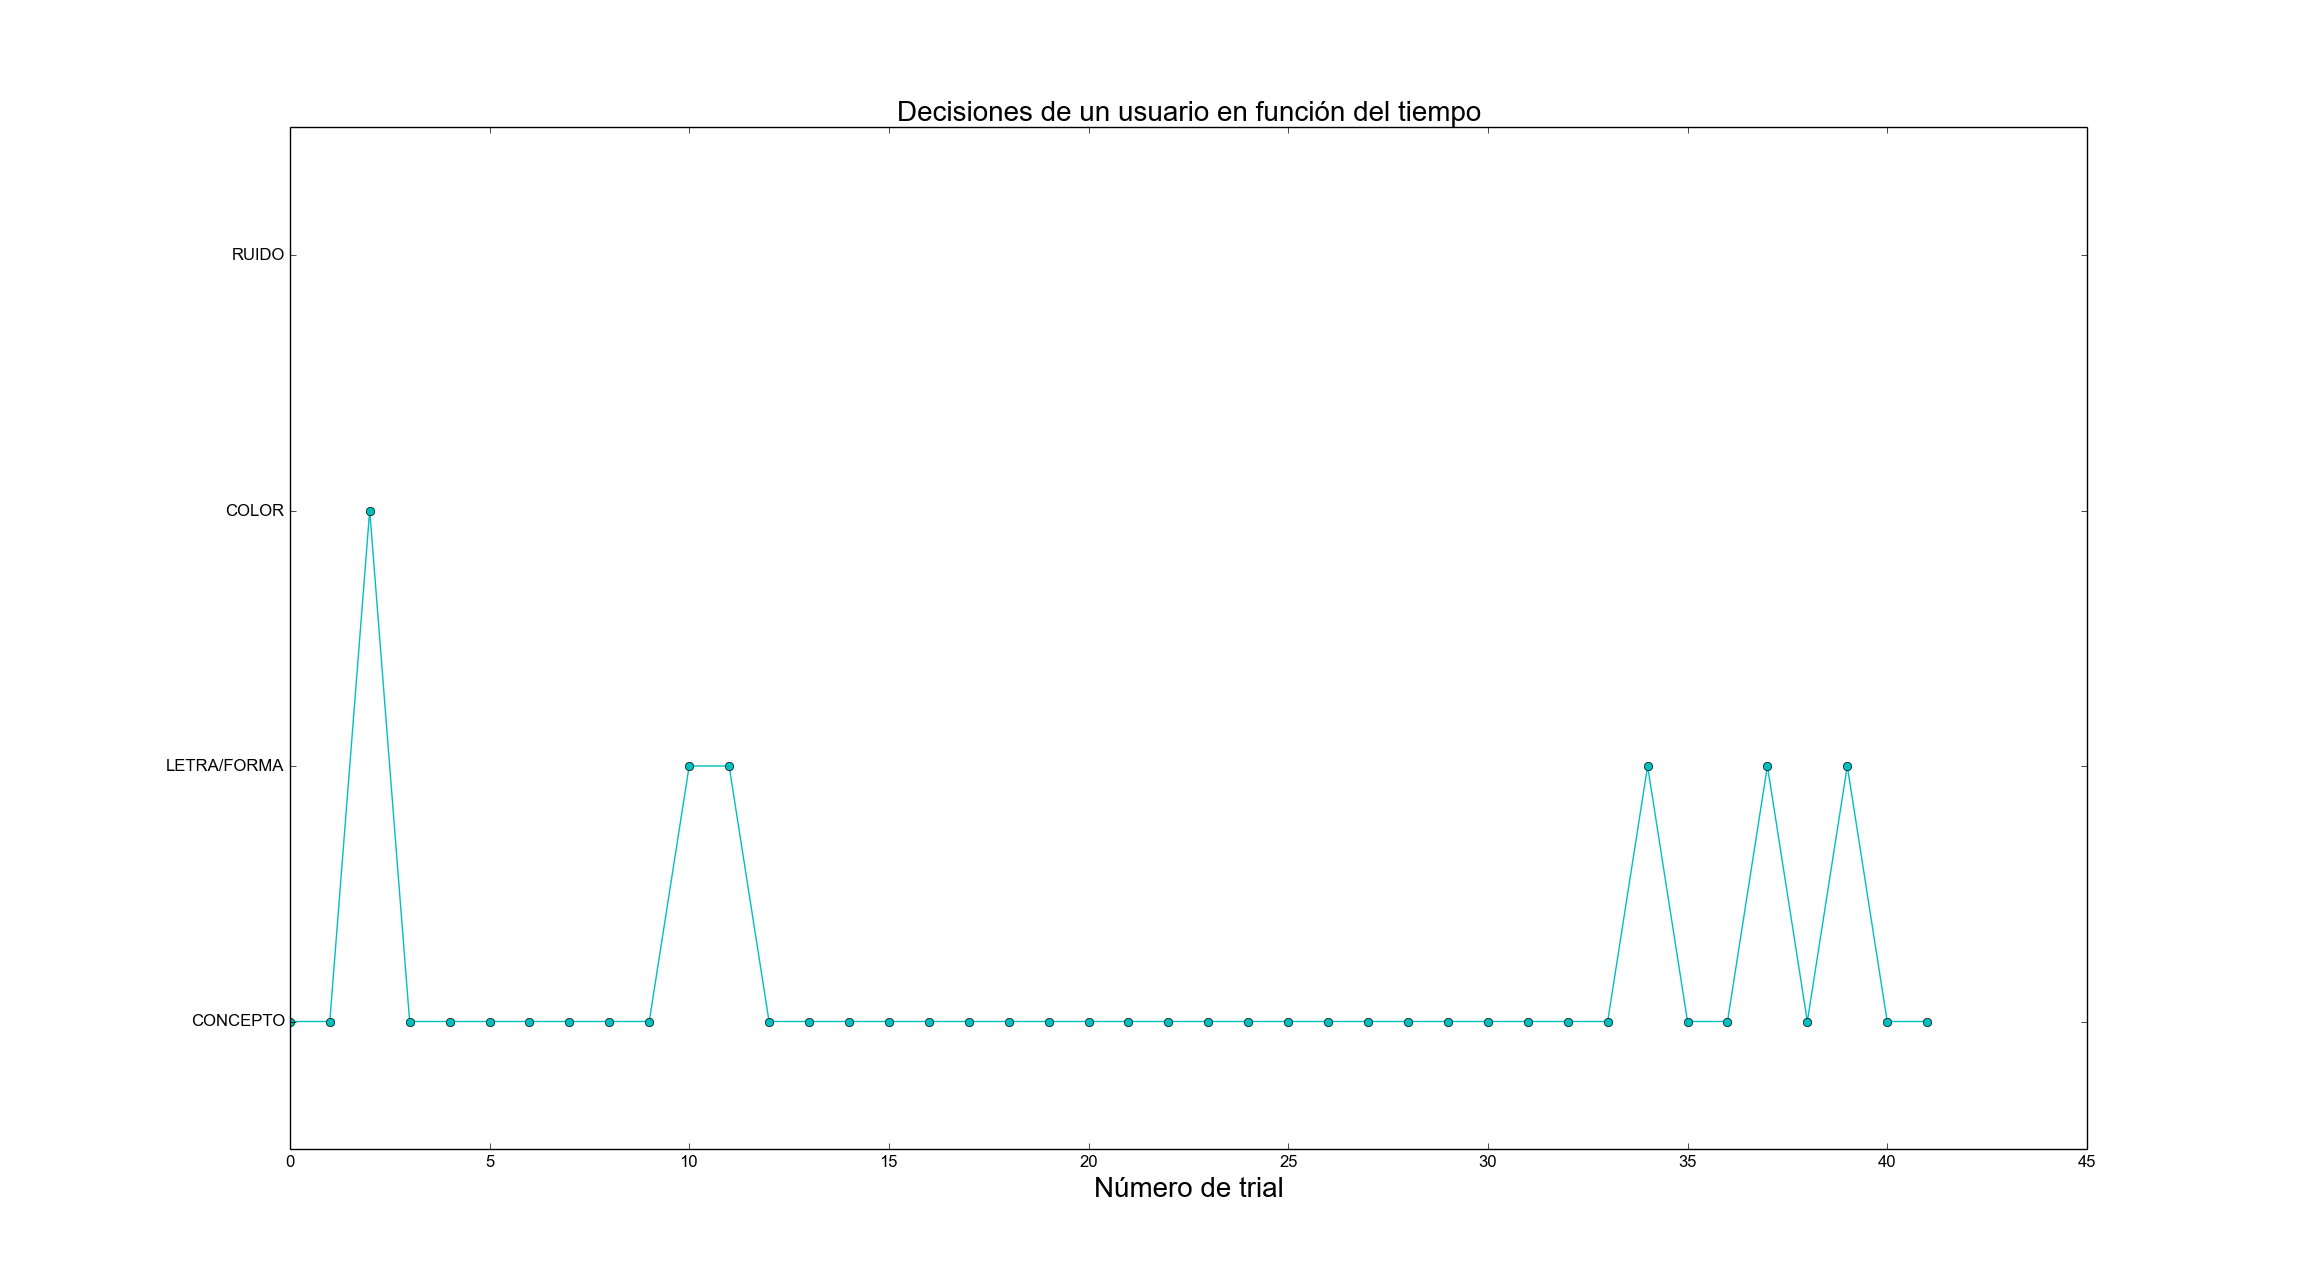
\includegraphics[scale=0.108]{user5.png}
  \end{minipage}
\end{figure}
\end{frame}

\begin{frame}
\begin{figure}[h]
 \centering
  \begin{minipage}[c]{1\textwidth}
	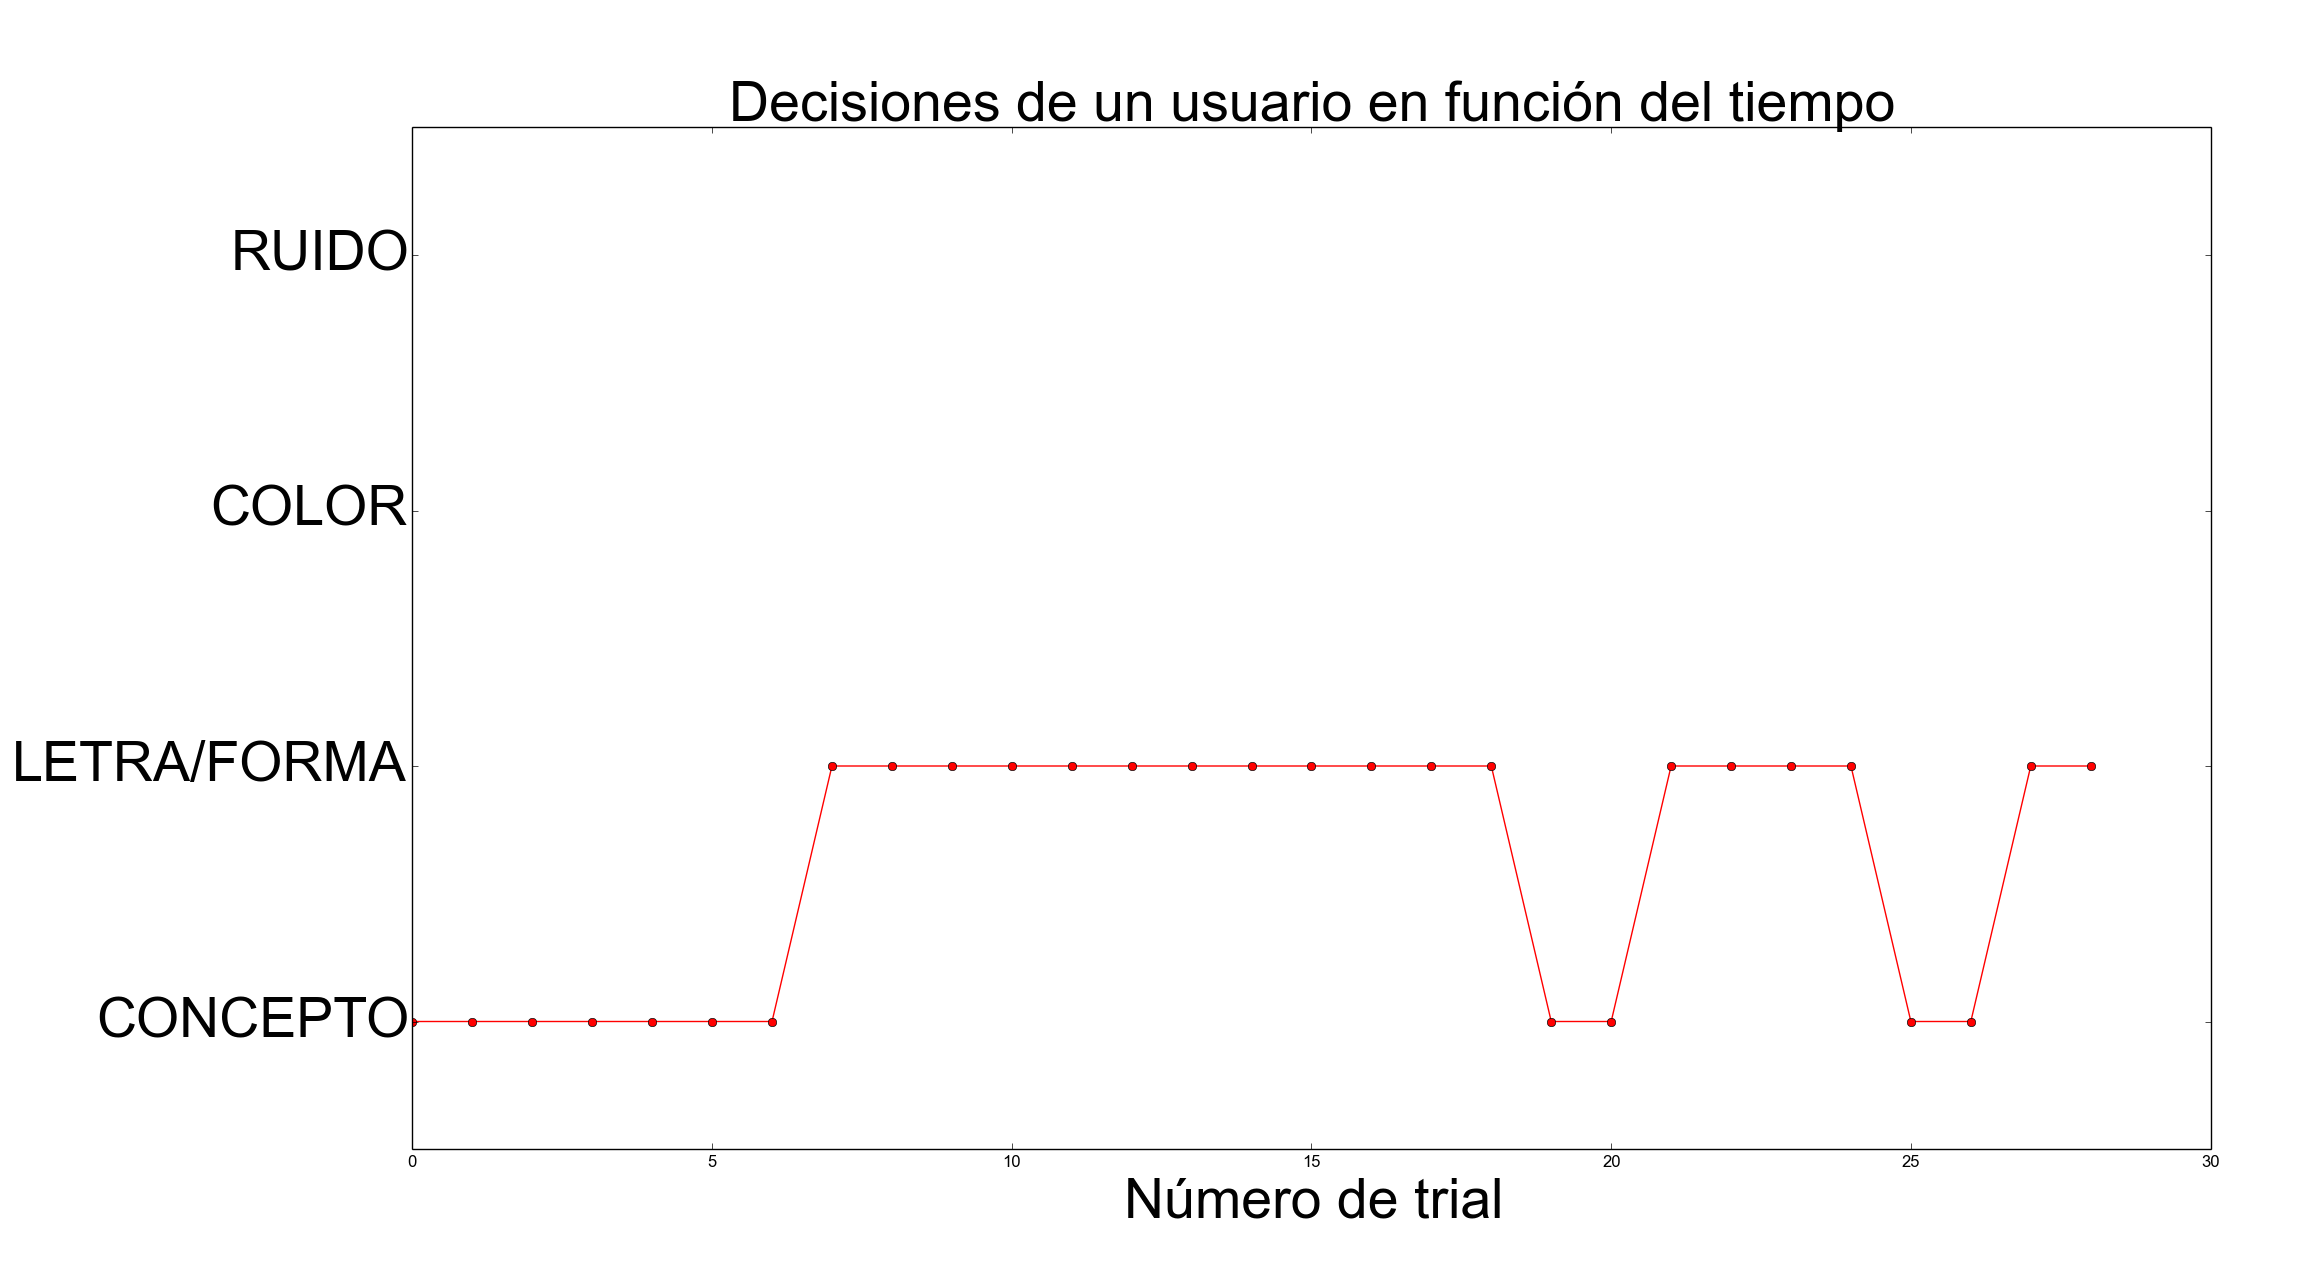
\includegraphics[scale=0.108]{user1.png}
	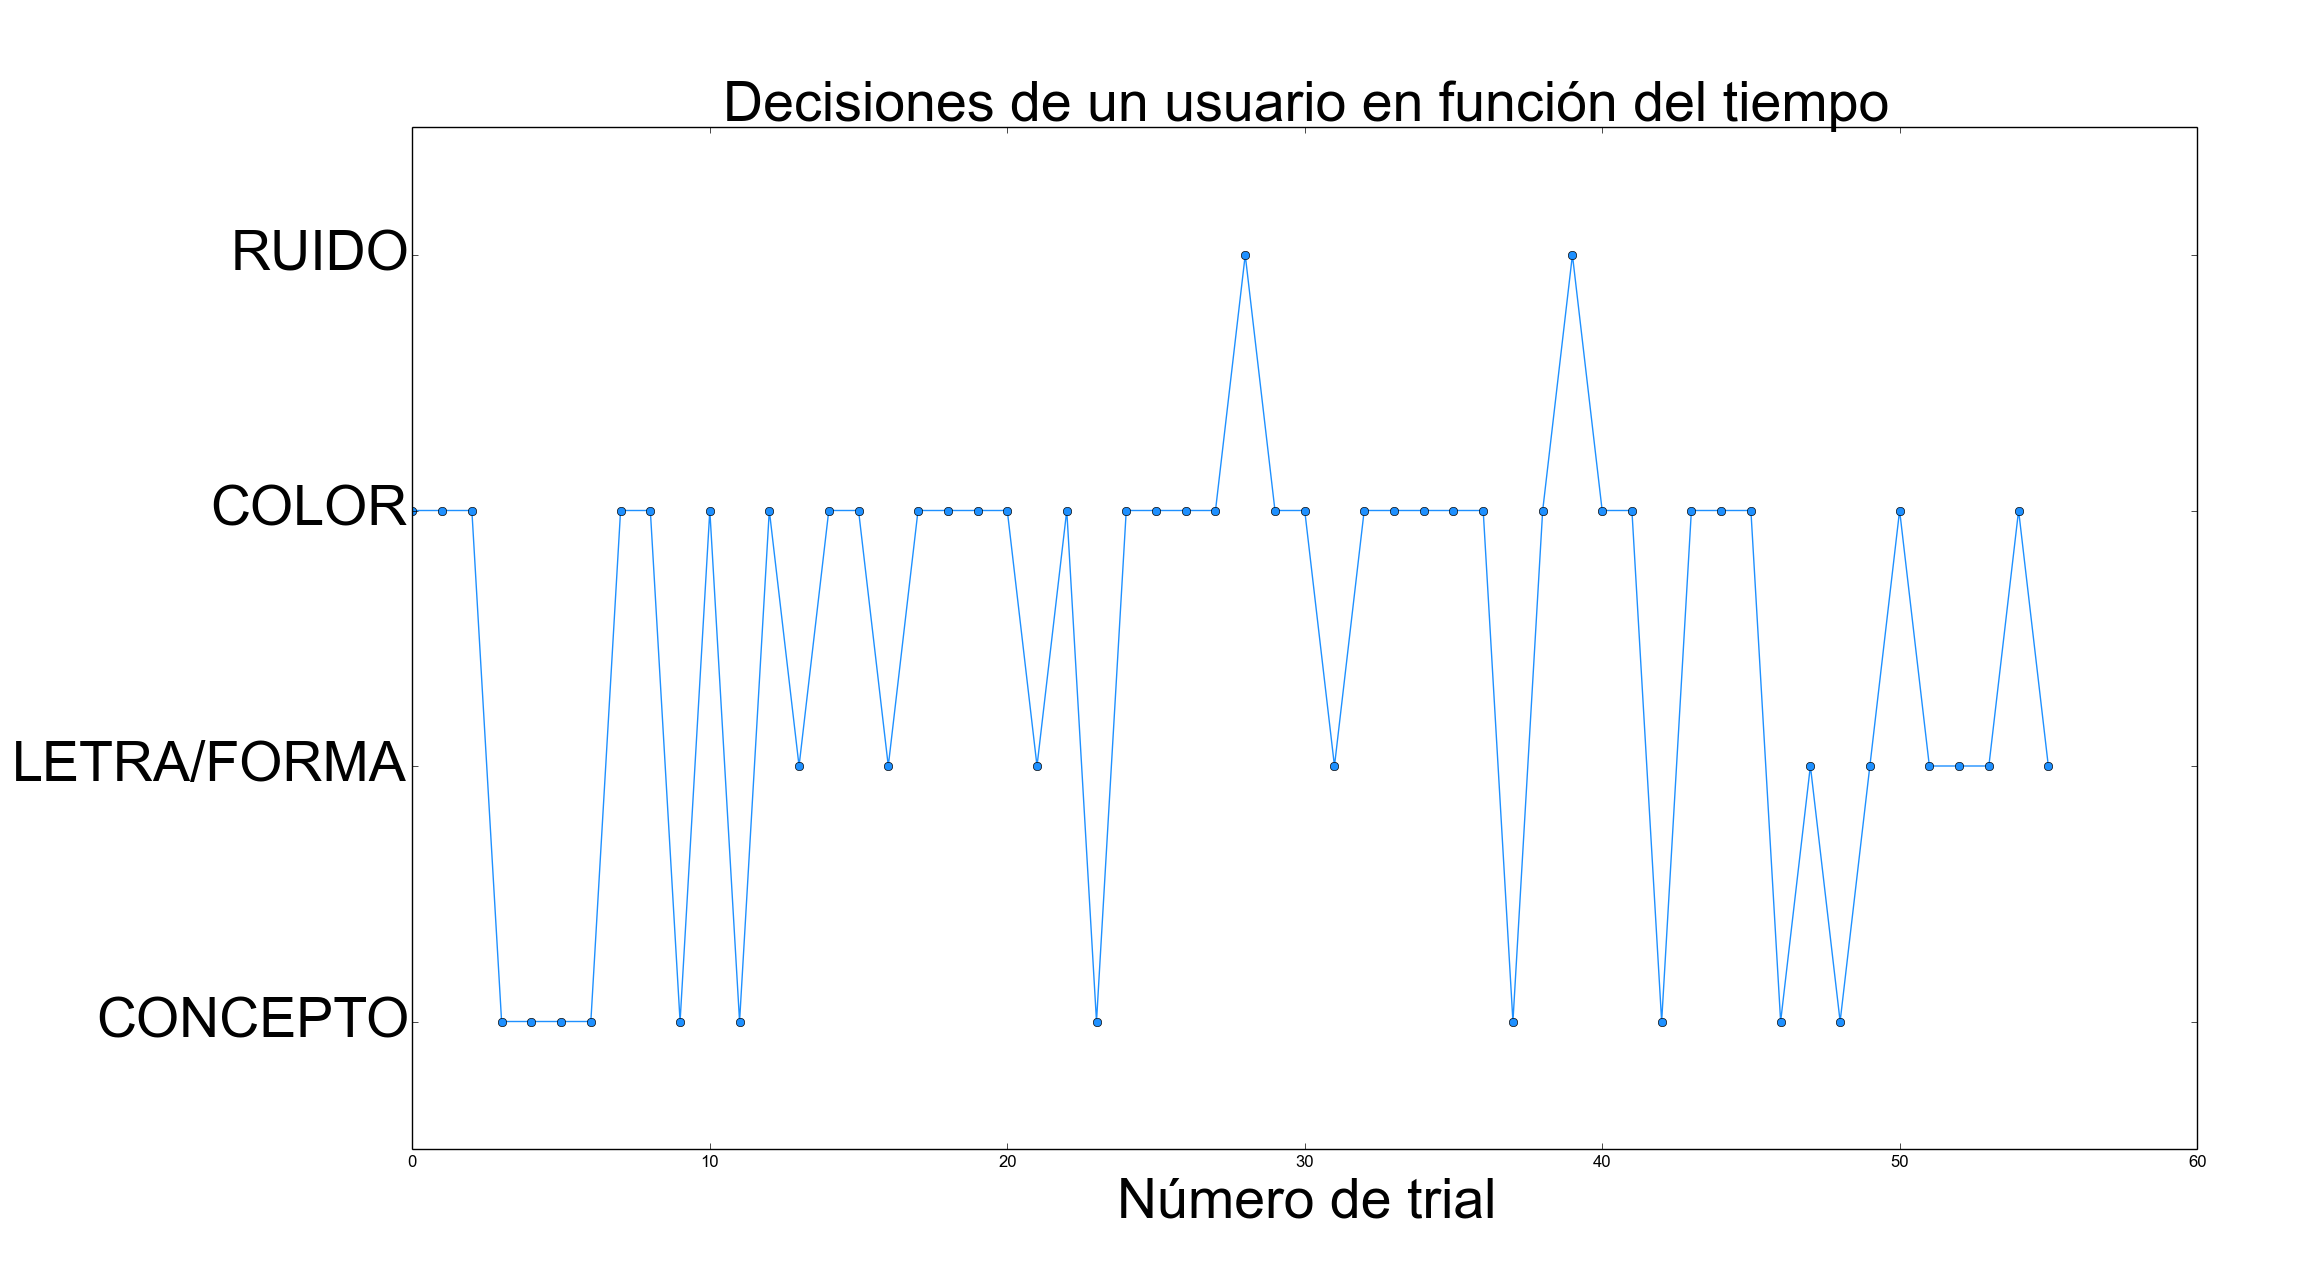
\includegraphics[scale=0.108]{user14.png}
  \end{minipage}
  \begin{minipage}[c]{1\textwidth}
	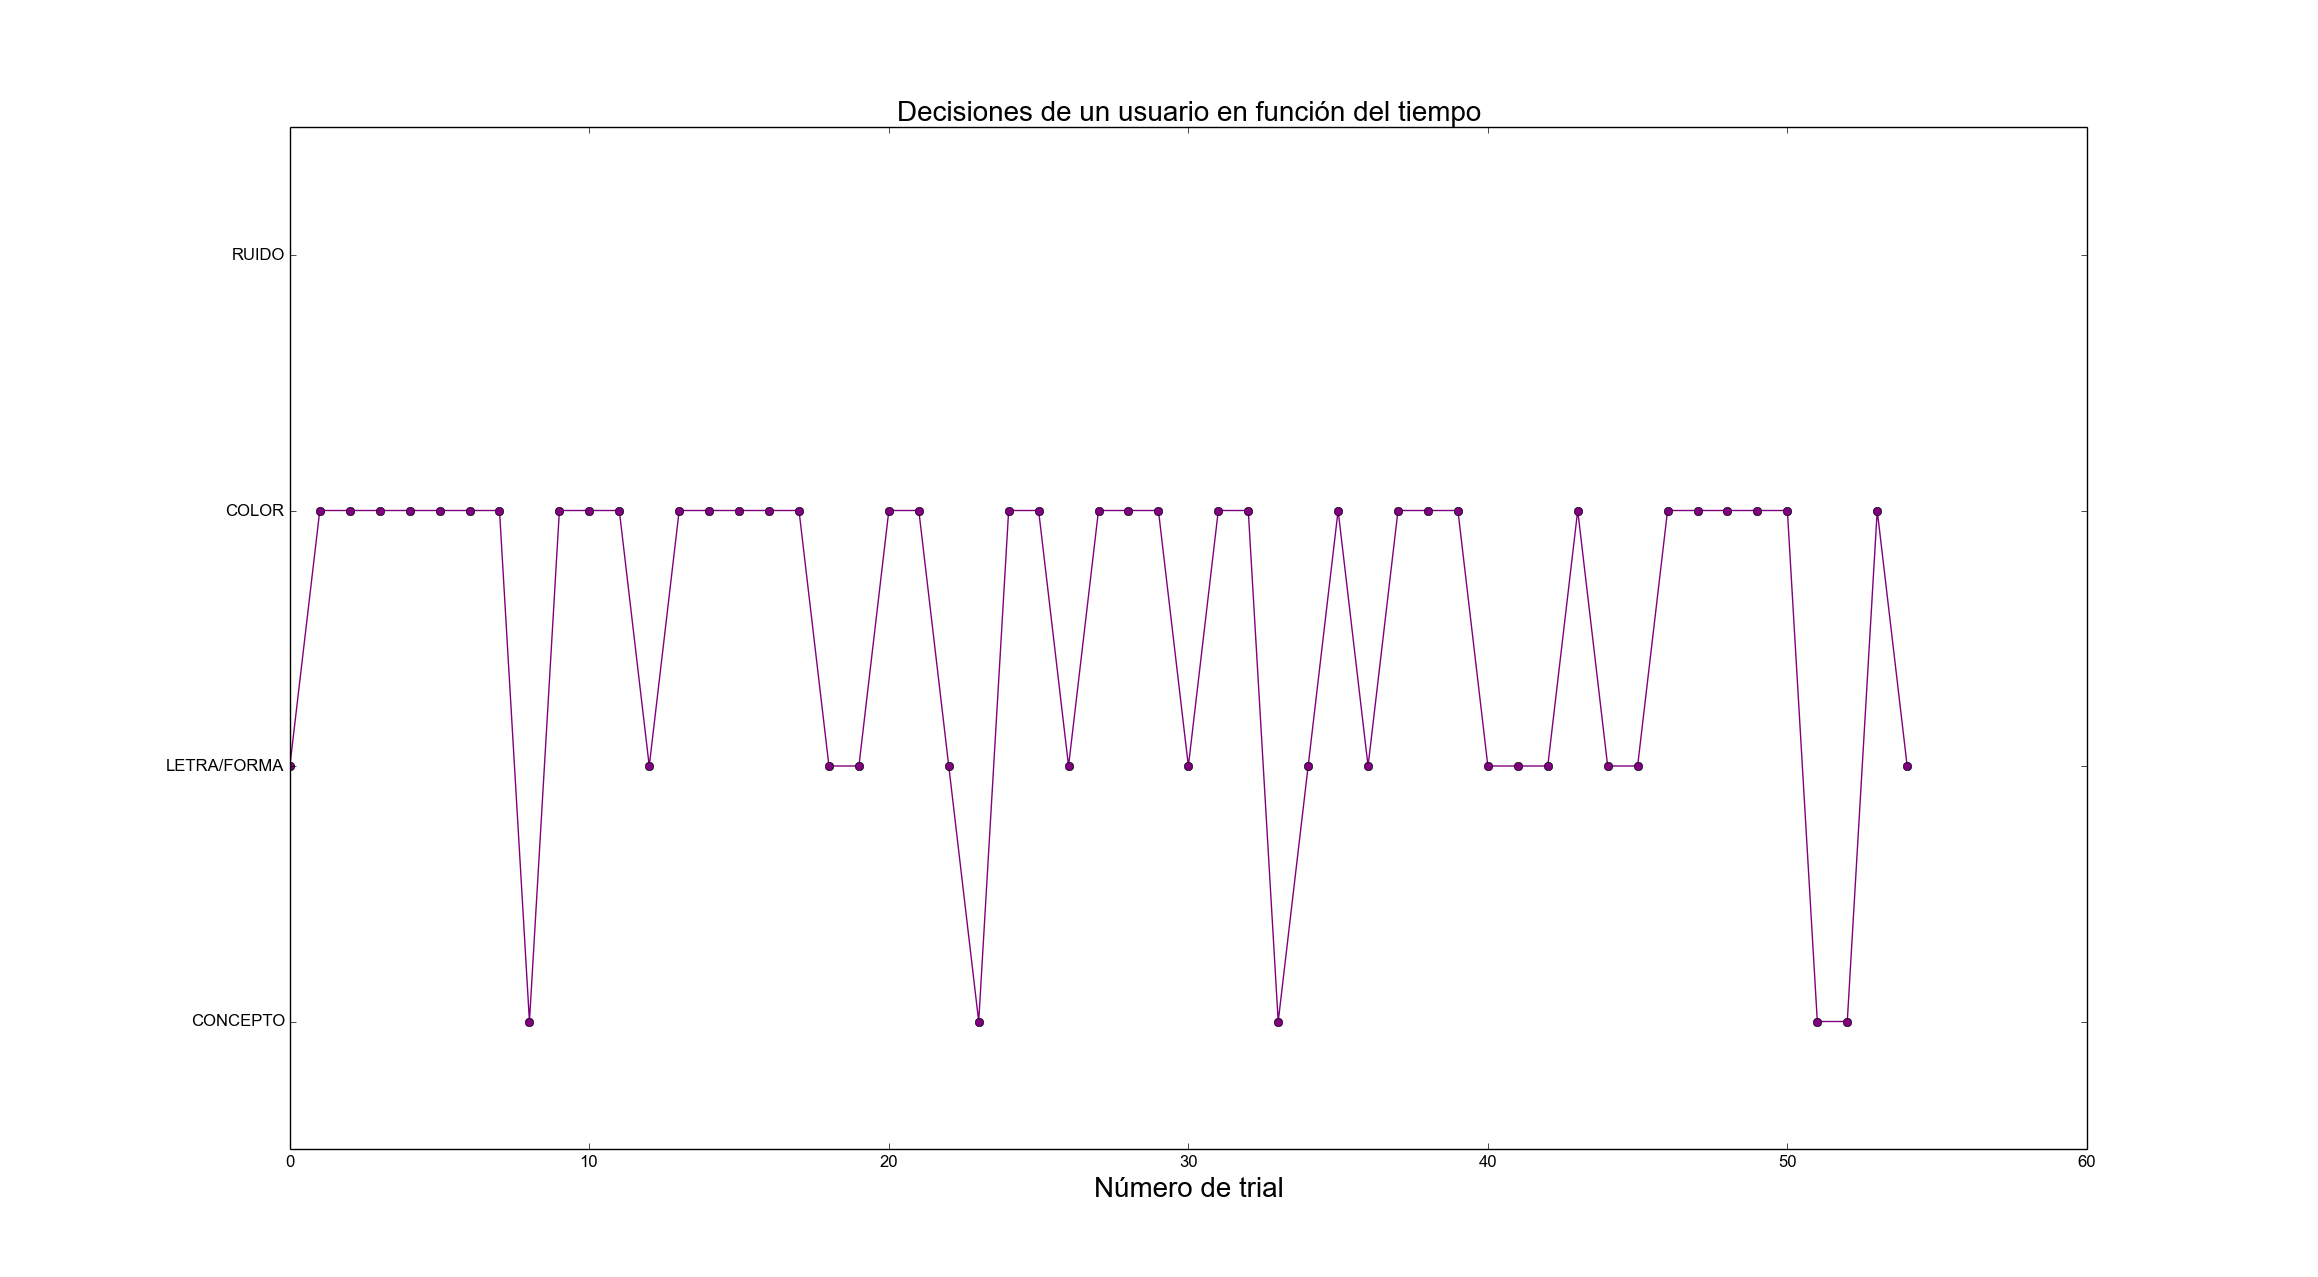
\includegraphics[scale=0.108]{user6.png}
	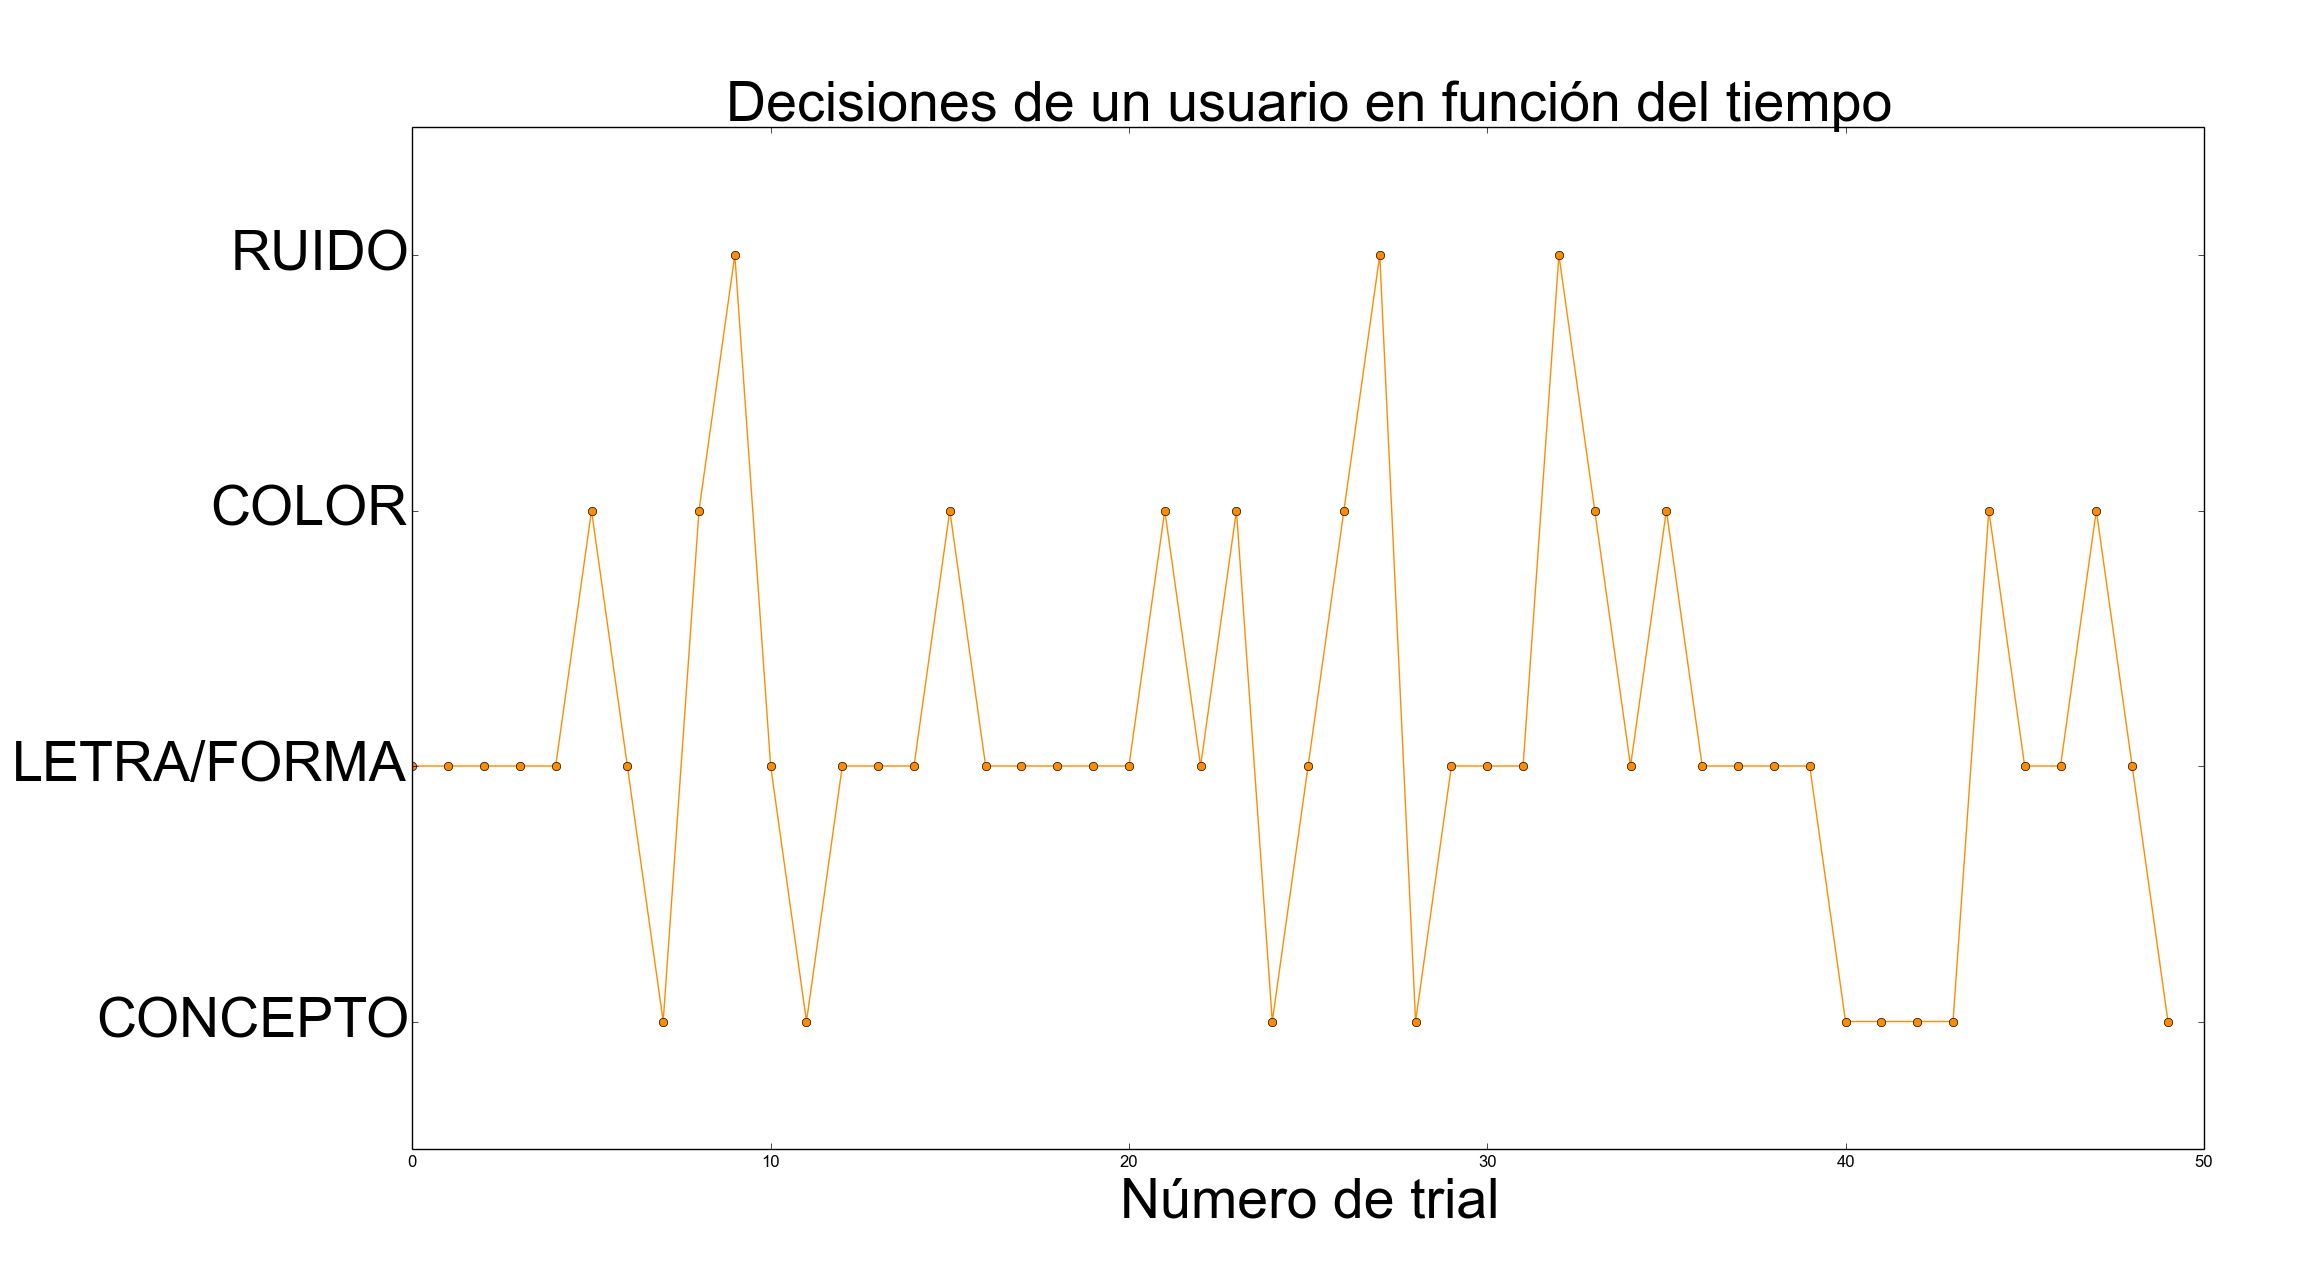
\includegraphics[scale=0.108]{user7.png}
  \end{minipage}
\end{figure}
\end{frame}

\begin{frame}
\begin{figure}[h]
 \centering
  \begin{minipage}[c]{1\textwidth}
	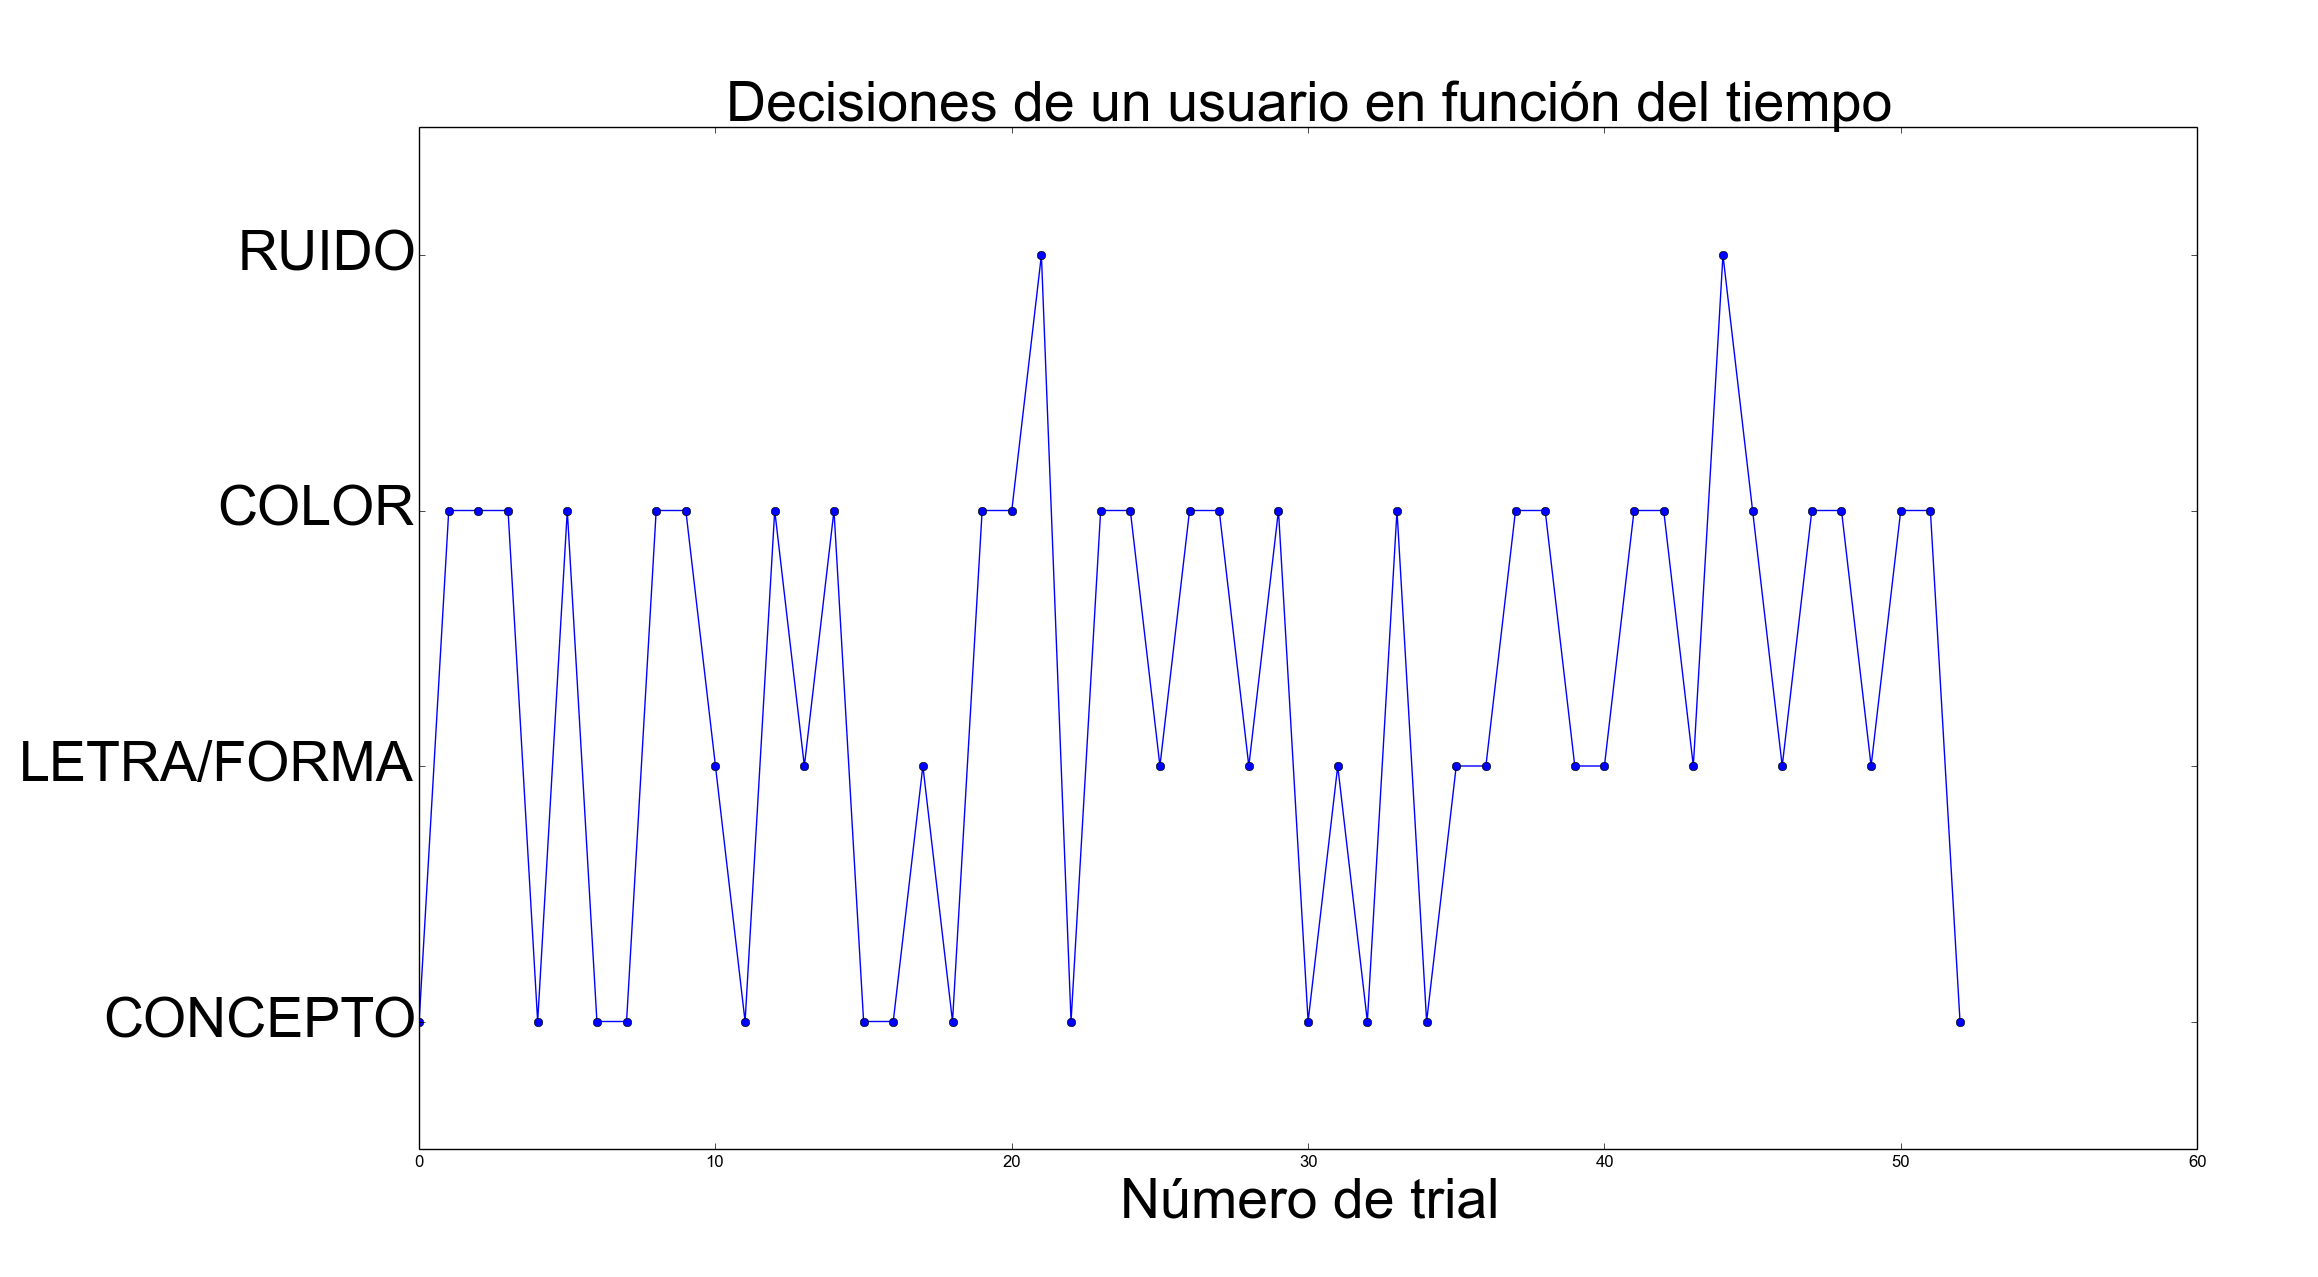
\includegraphics[scale=0.108]{user3.png}
	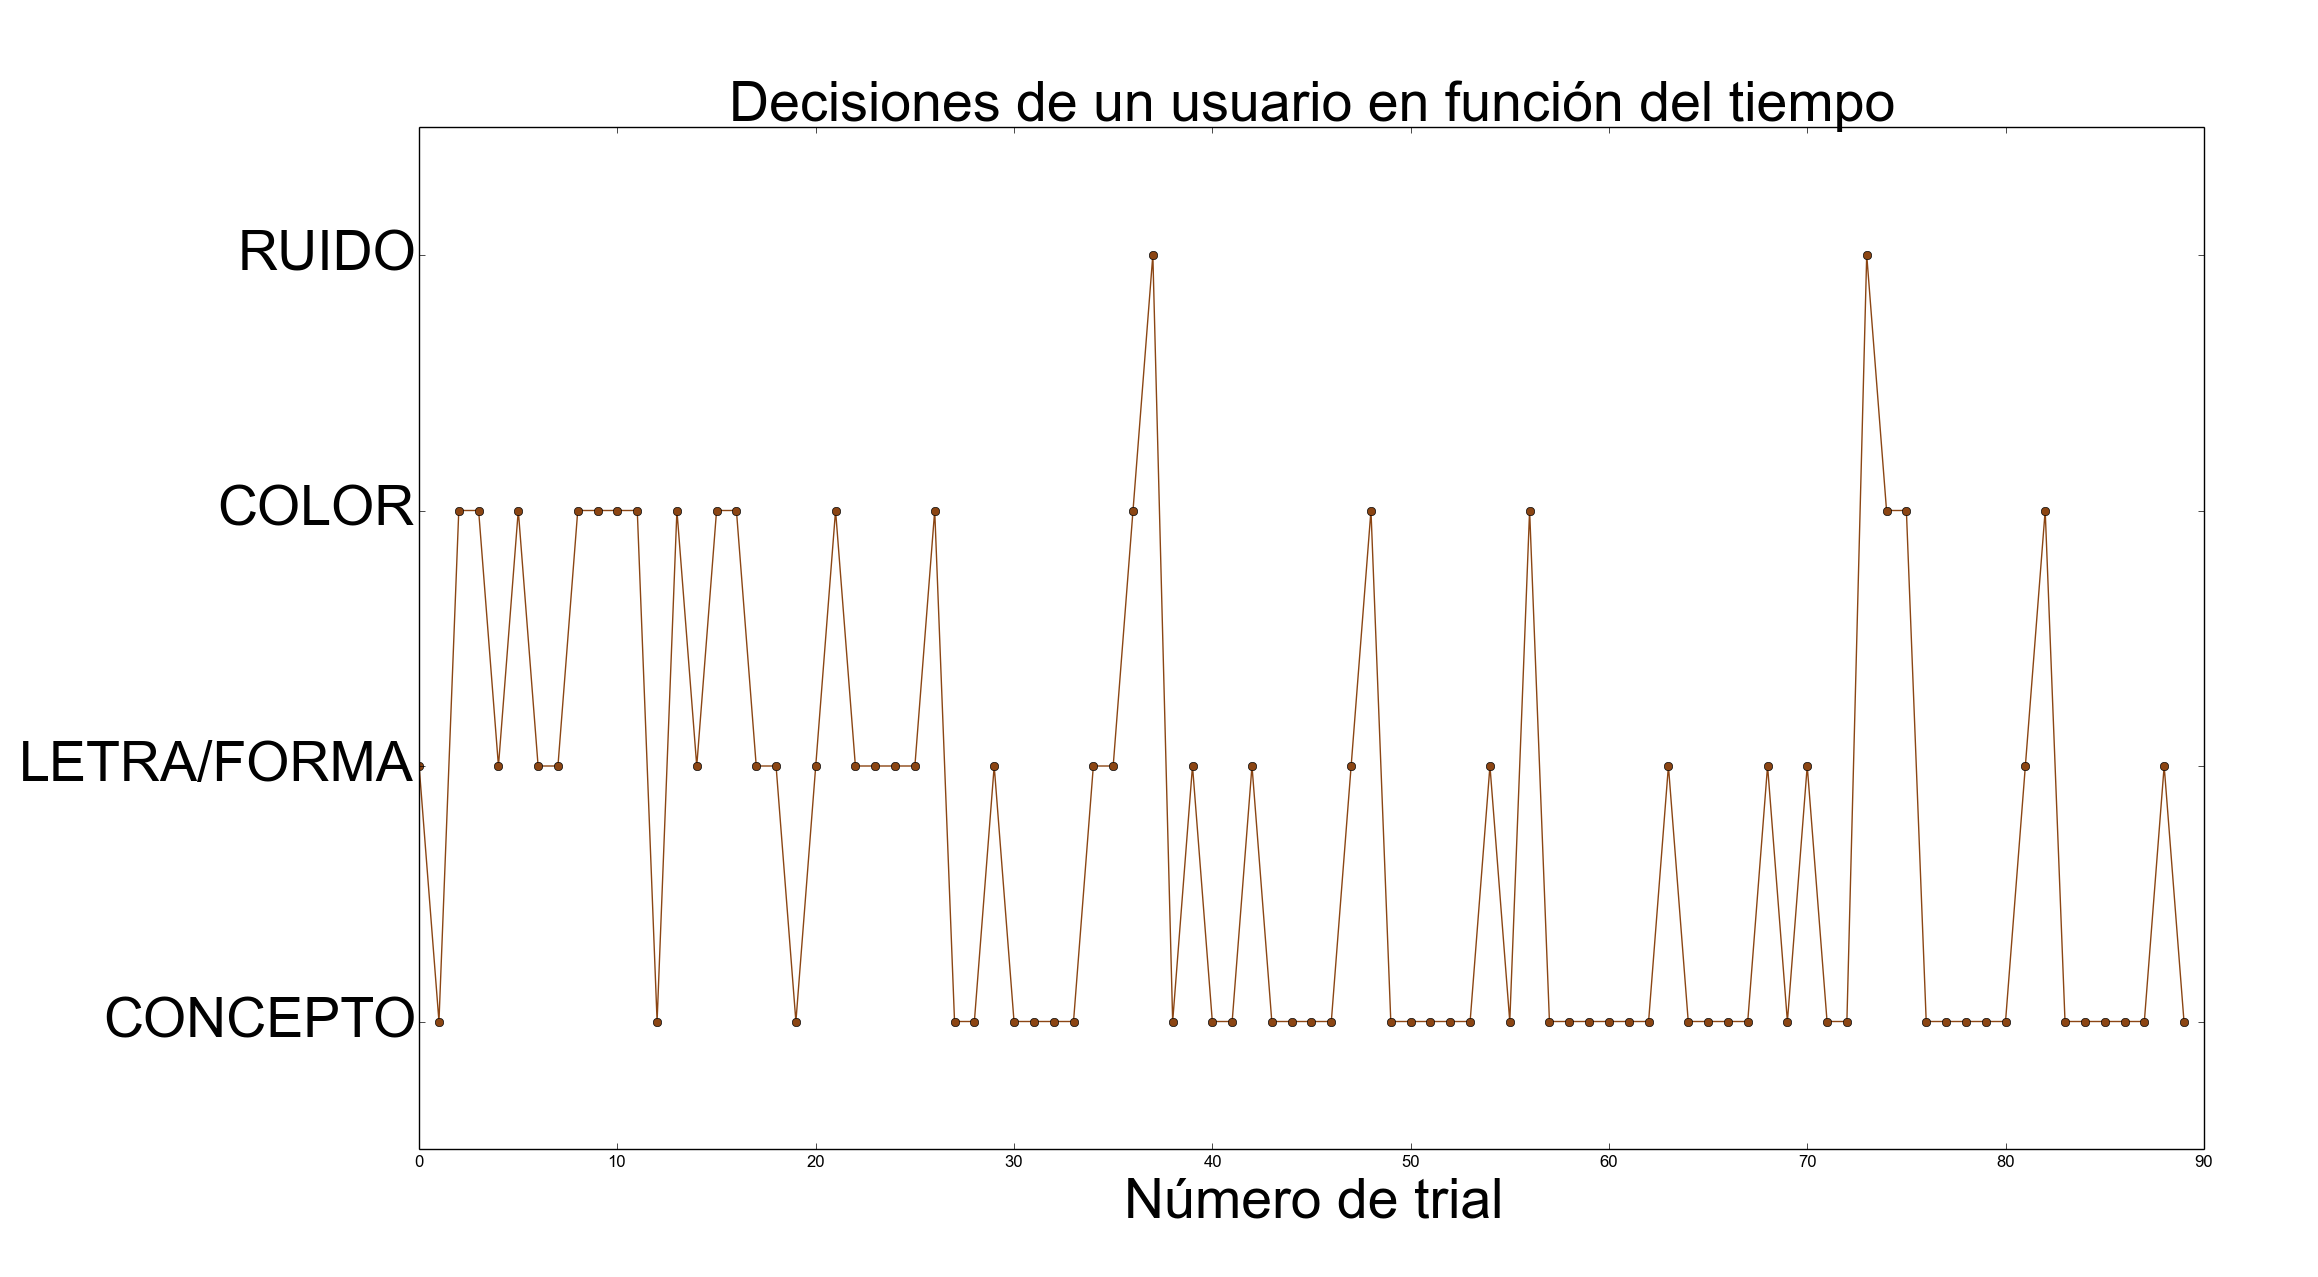
\includegraphics[scale=0.108]{user13.png}
  \end{minipage}
  \begin{minipage}[c]{1\textwidth}
	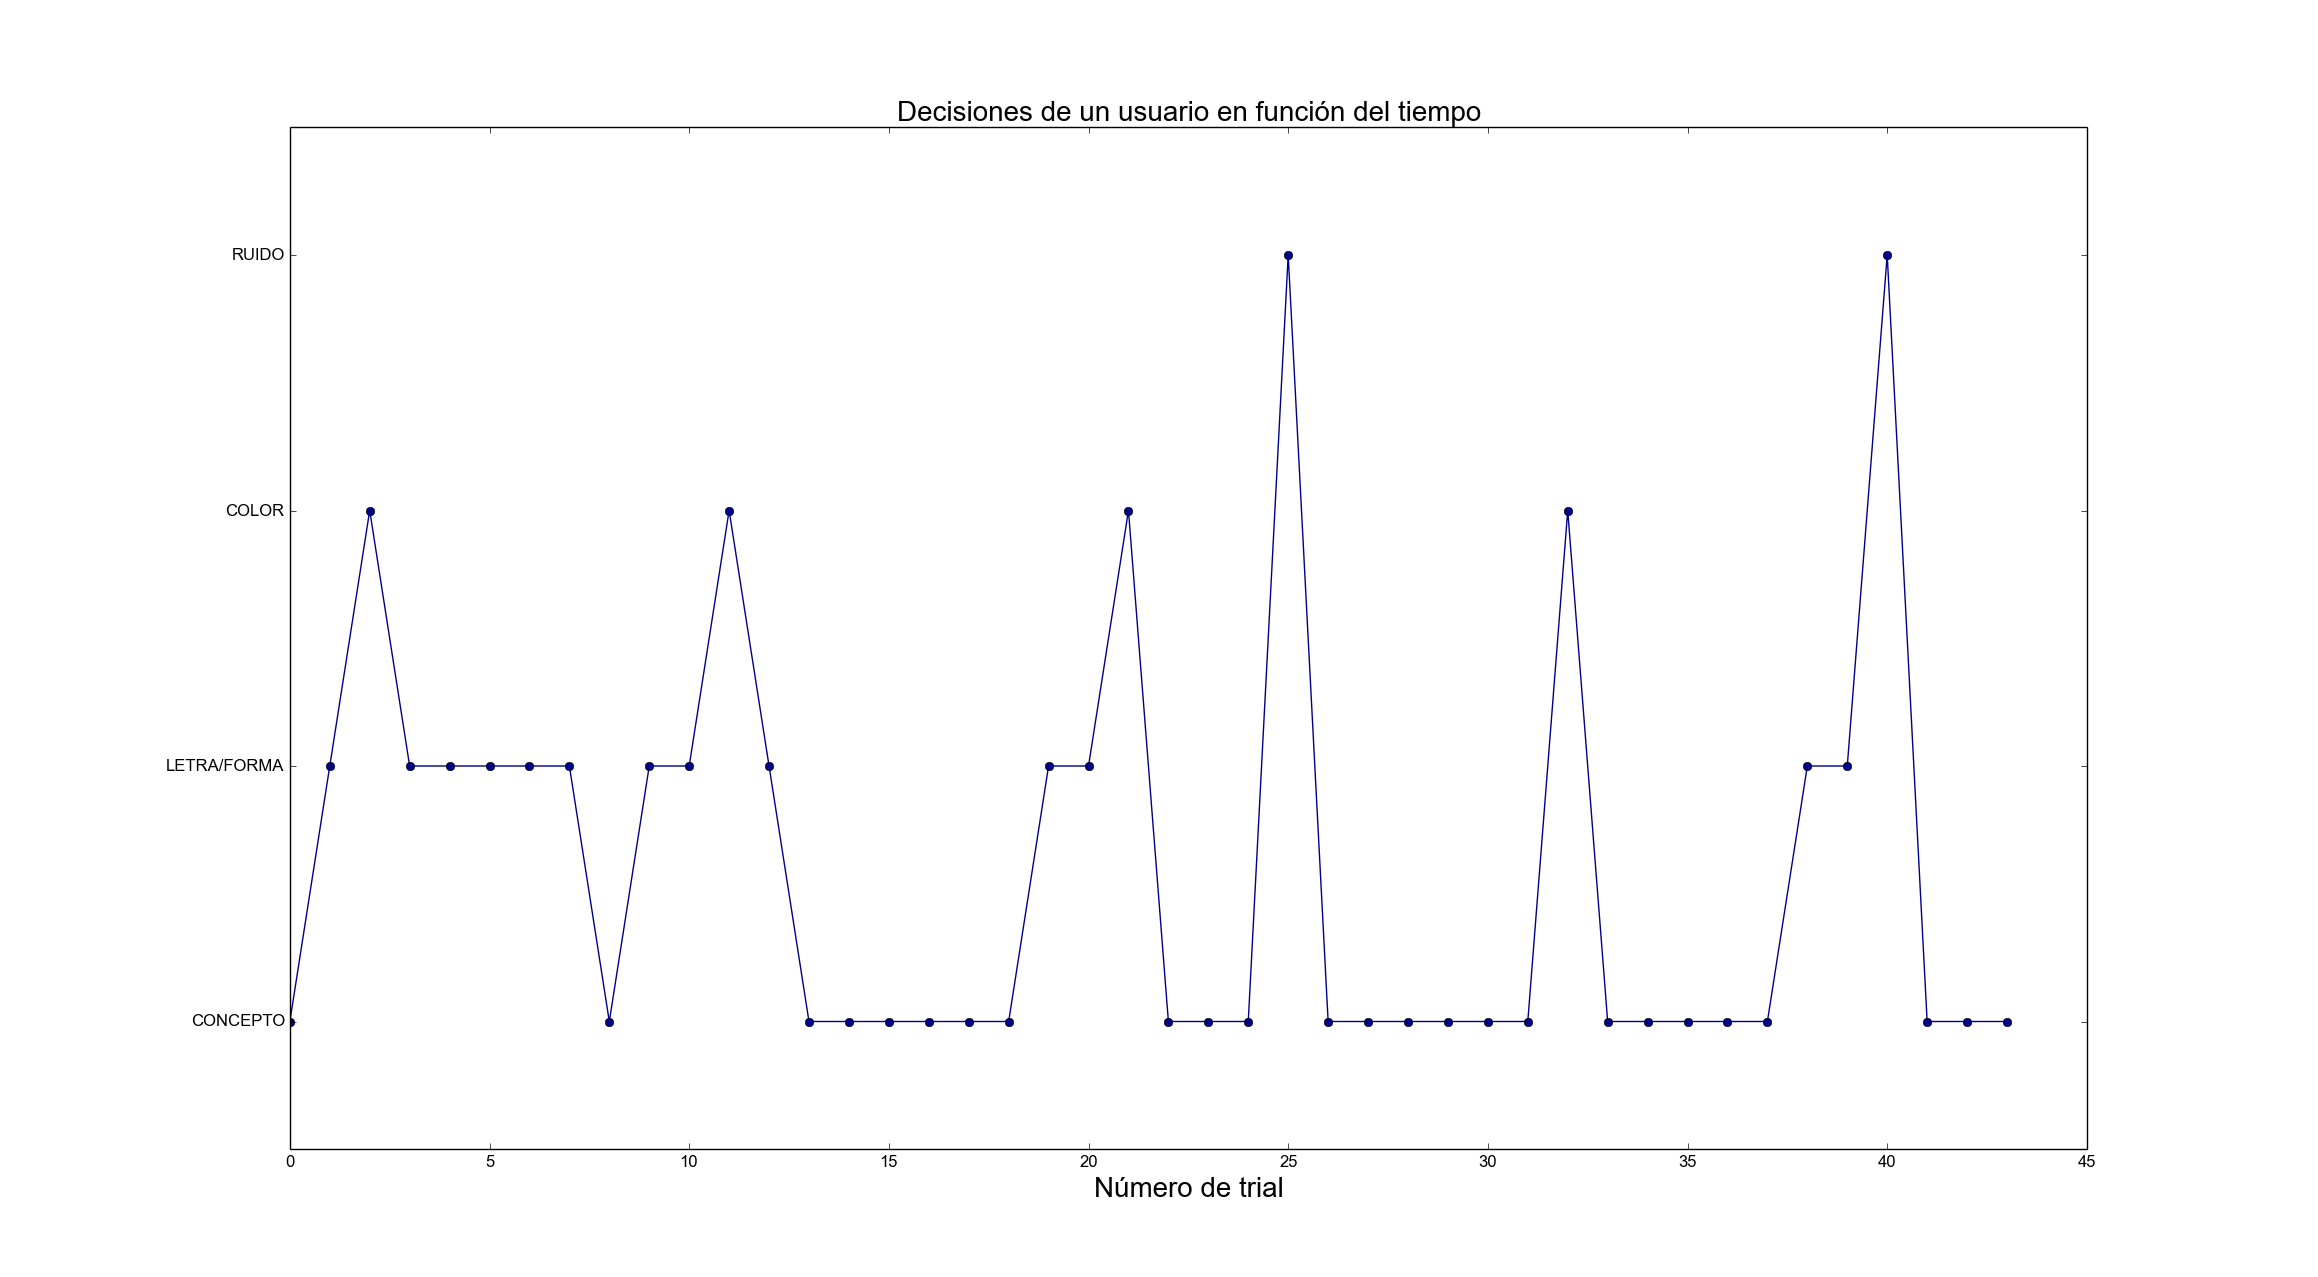
\includegraphics[scale=0.108]{user8.png}
	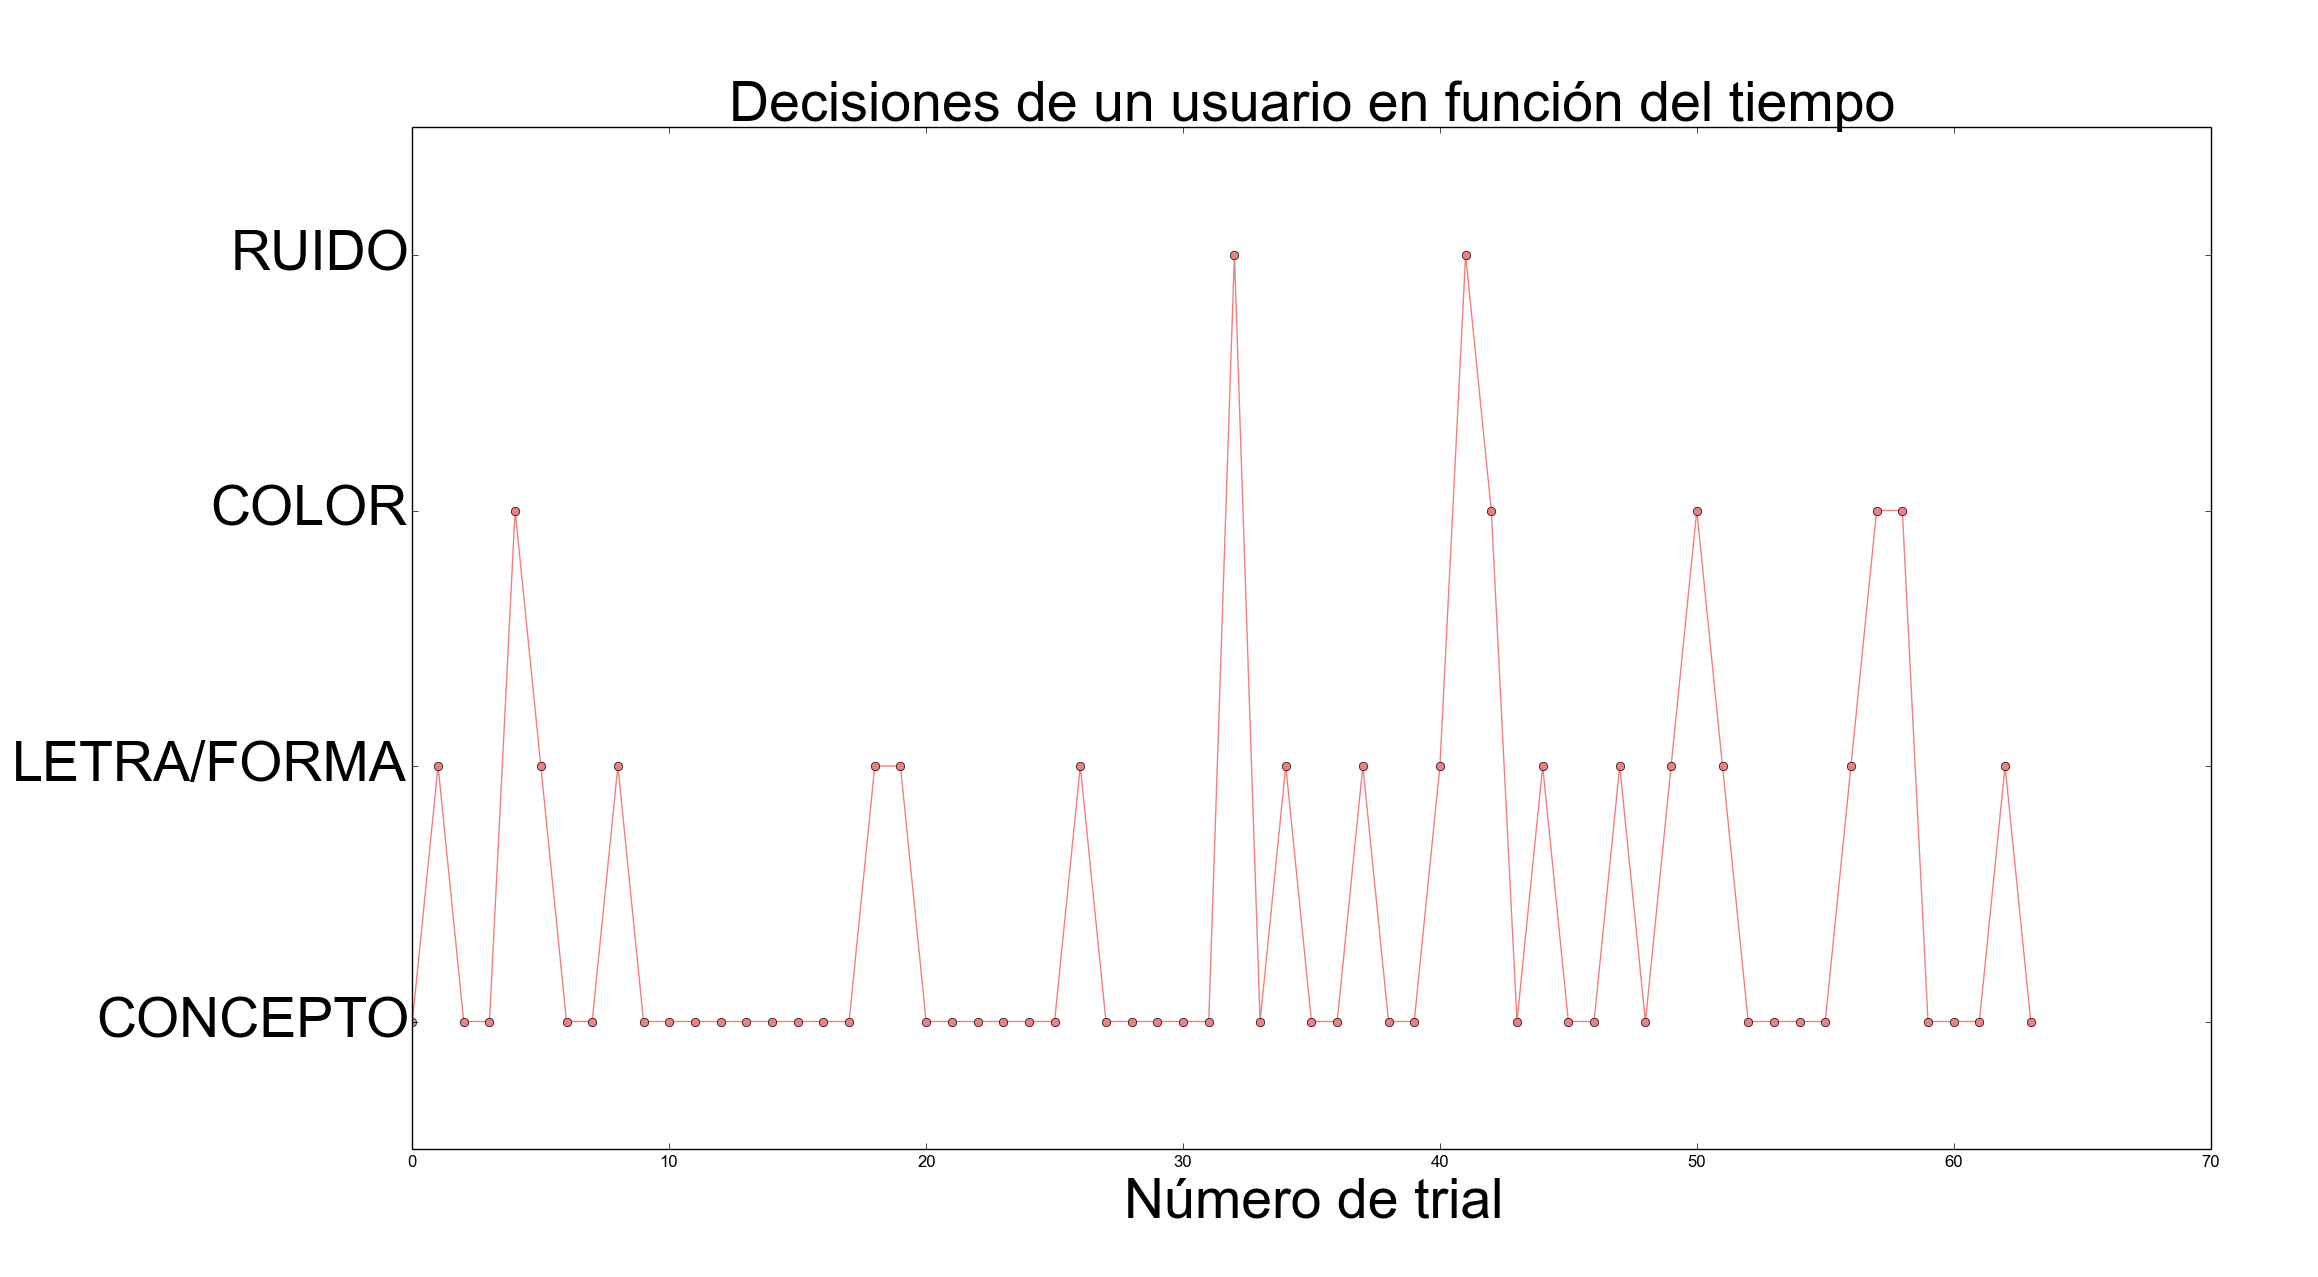
\includegraphics[scale=0.108]{user11.png}
  \end{minipage}
\end{figure}
\end{frame}

\subsection{Set Trials}

\begin{frame}
\begin{figure}[h]
 \centering
  \begin{minipage}[c]{1\textwidth}
	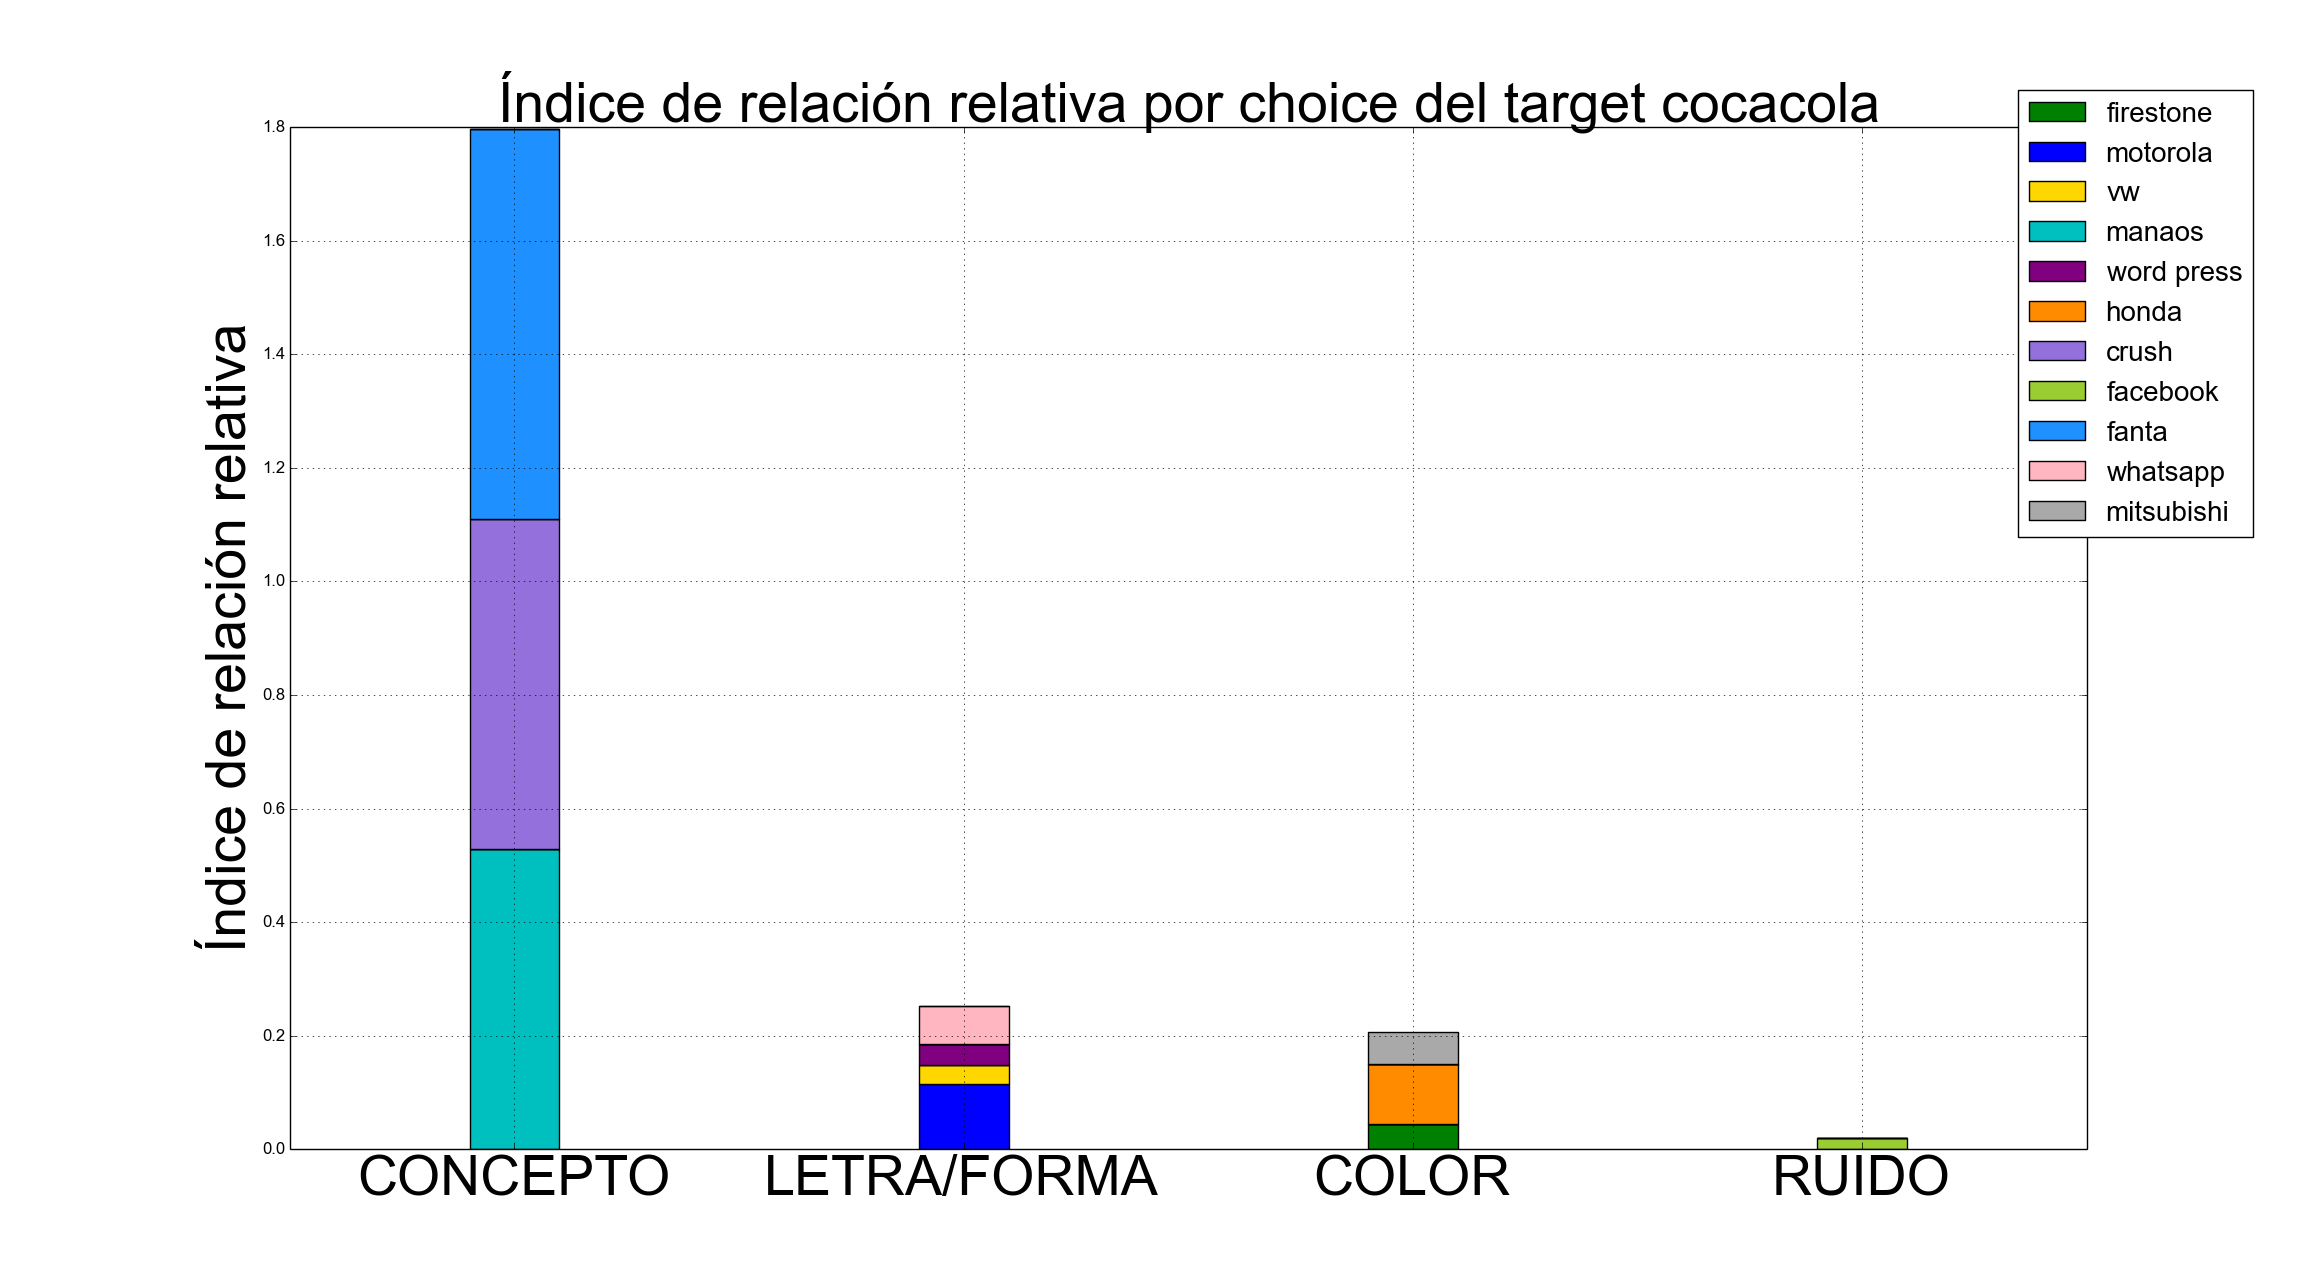
\includegraphics[scale=0.108]{cocacola.png}
	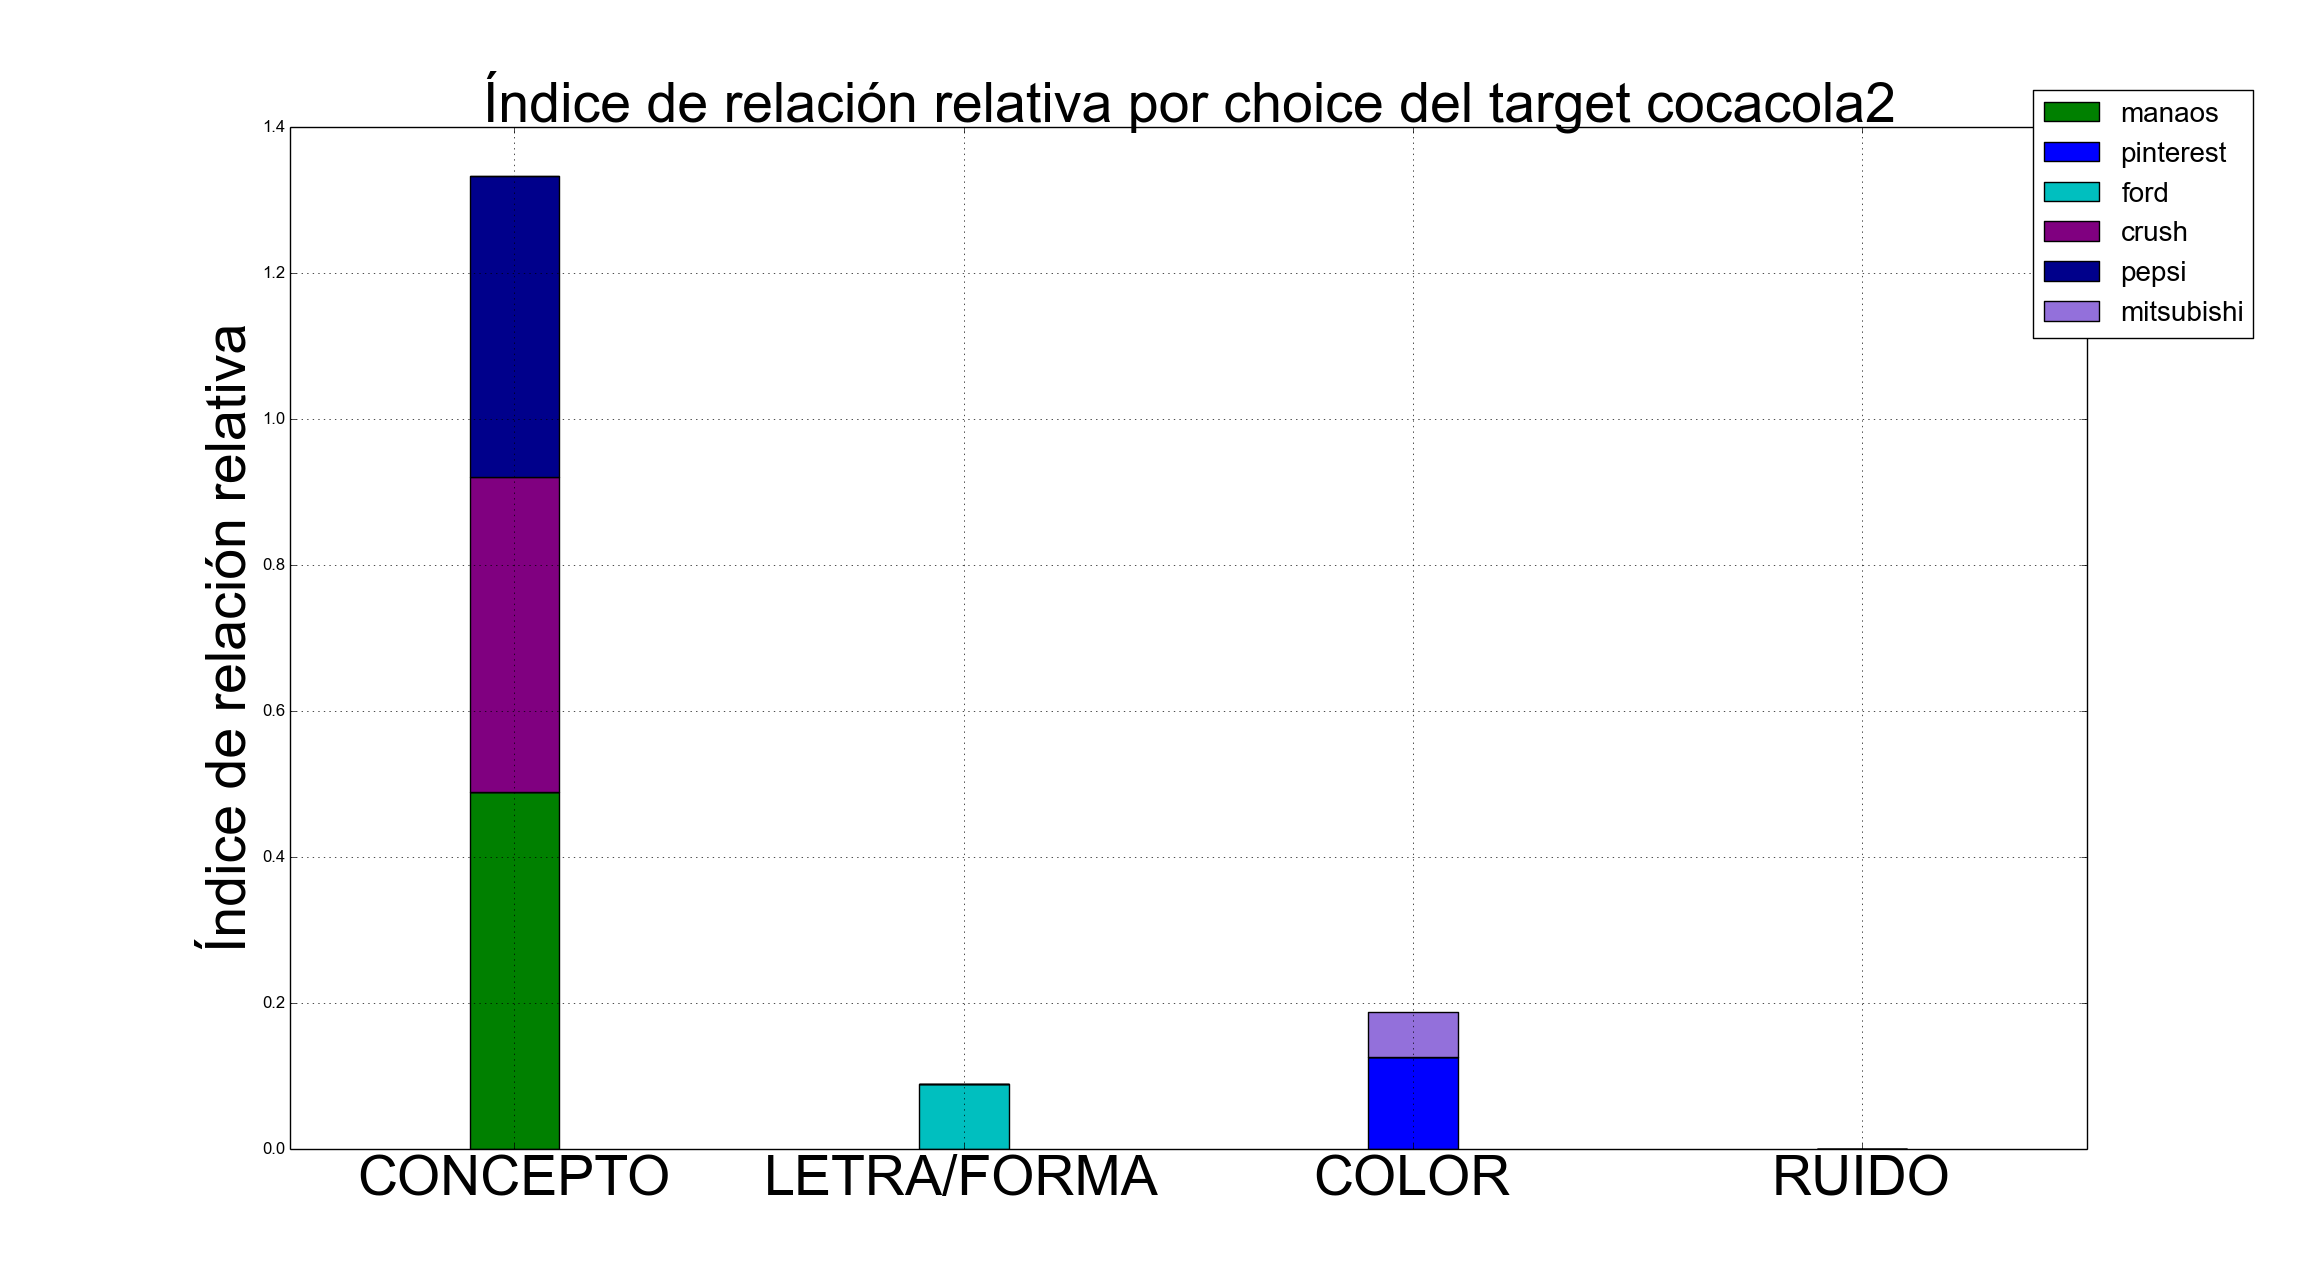
\includegraphics[scale=0.108]{cocacola2.png}
  \end{minipage}
  \begin{minipage}[c]{1\textwidth}
	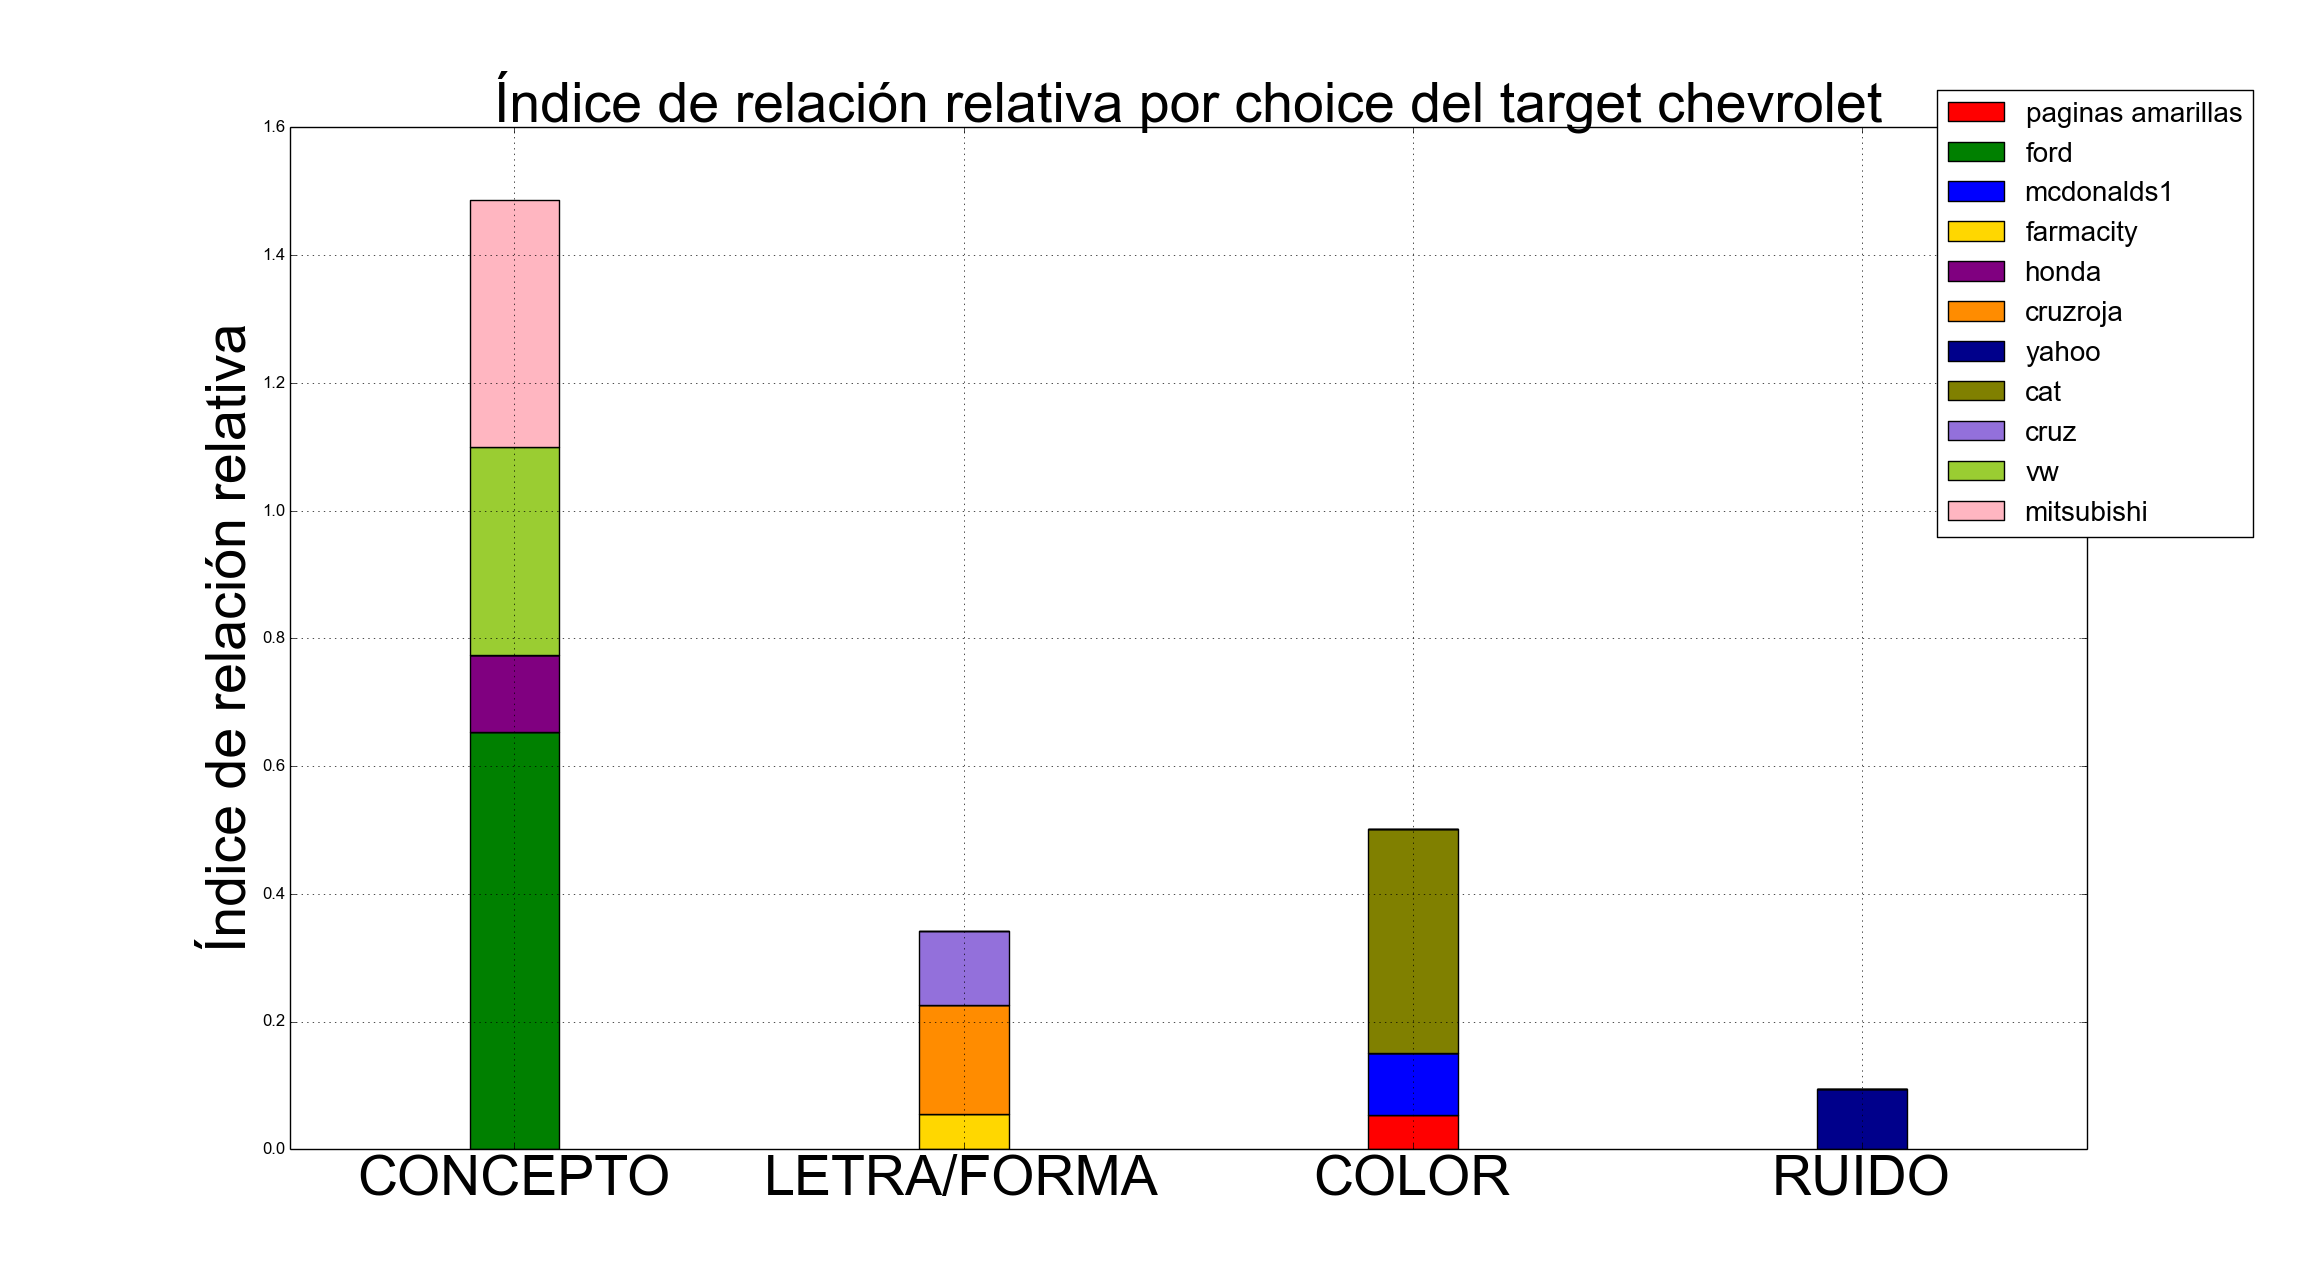
\includegraphics[scale=0.108]{chevrolet.png}
	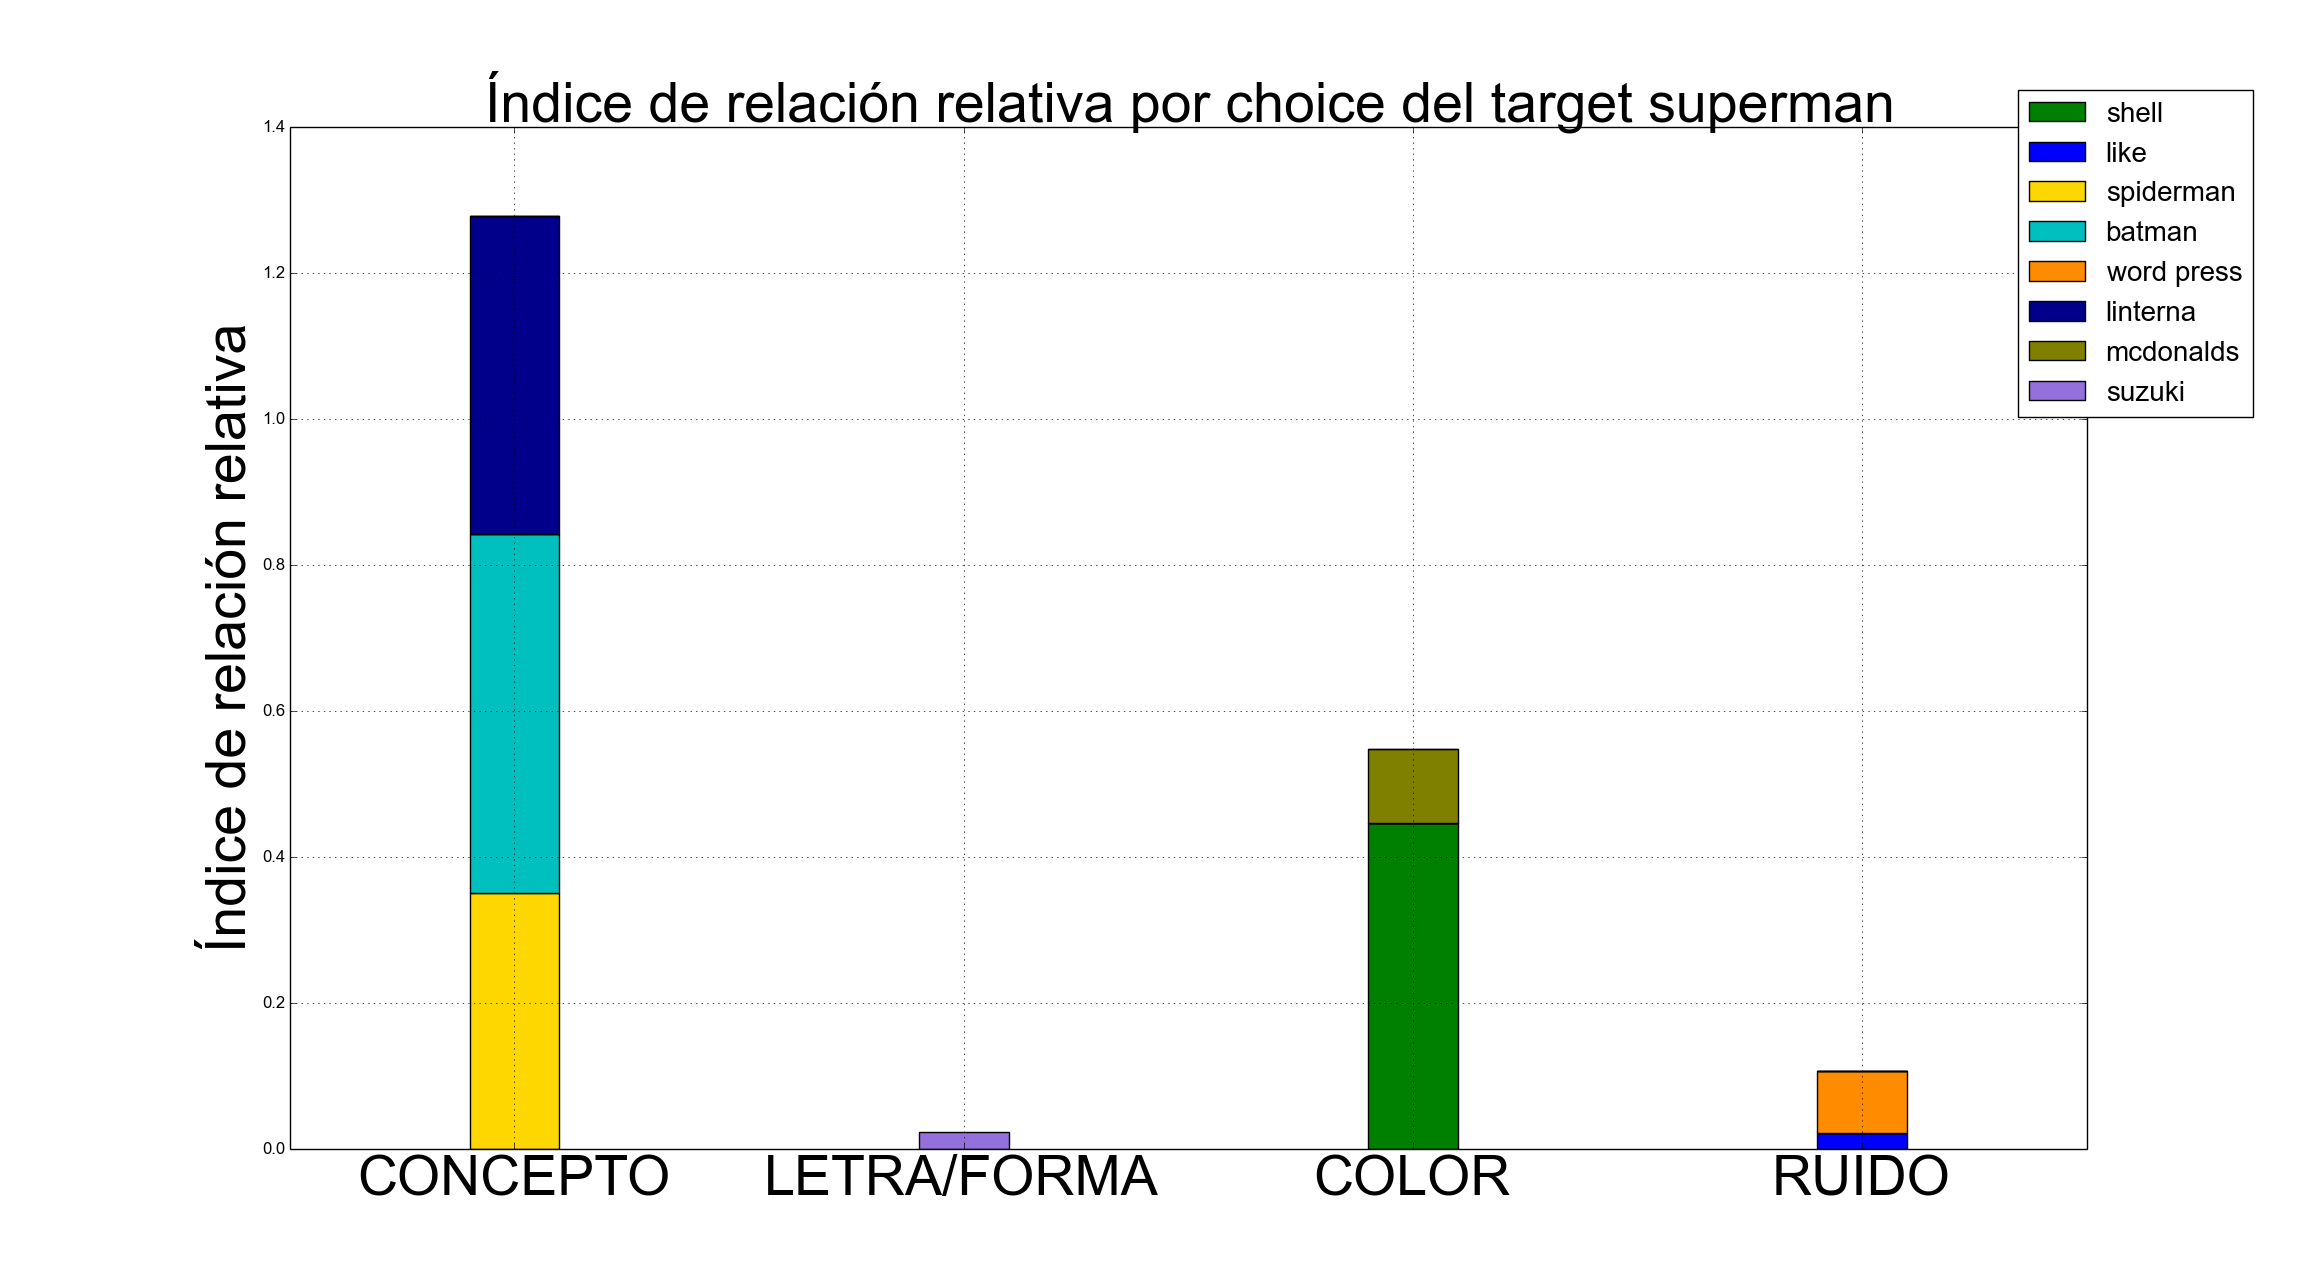
\includegraphics[scale=0.108]{superman.png}
  \end{minipage}
\end{figure}
\end{frame}

\begin{frame}
\begin{figure}[h]
 \centering
  \begin{minipage}[c]{1\textwidth}
	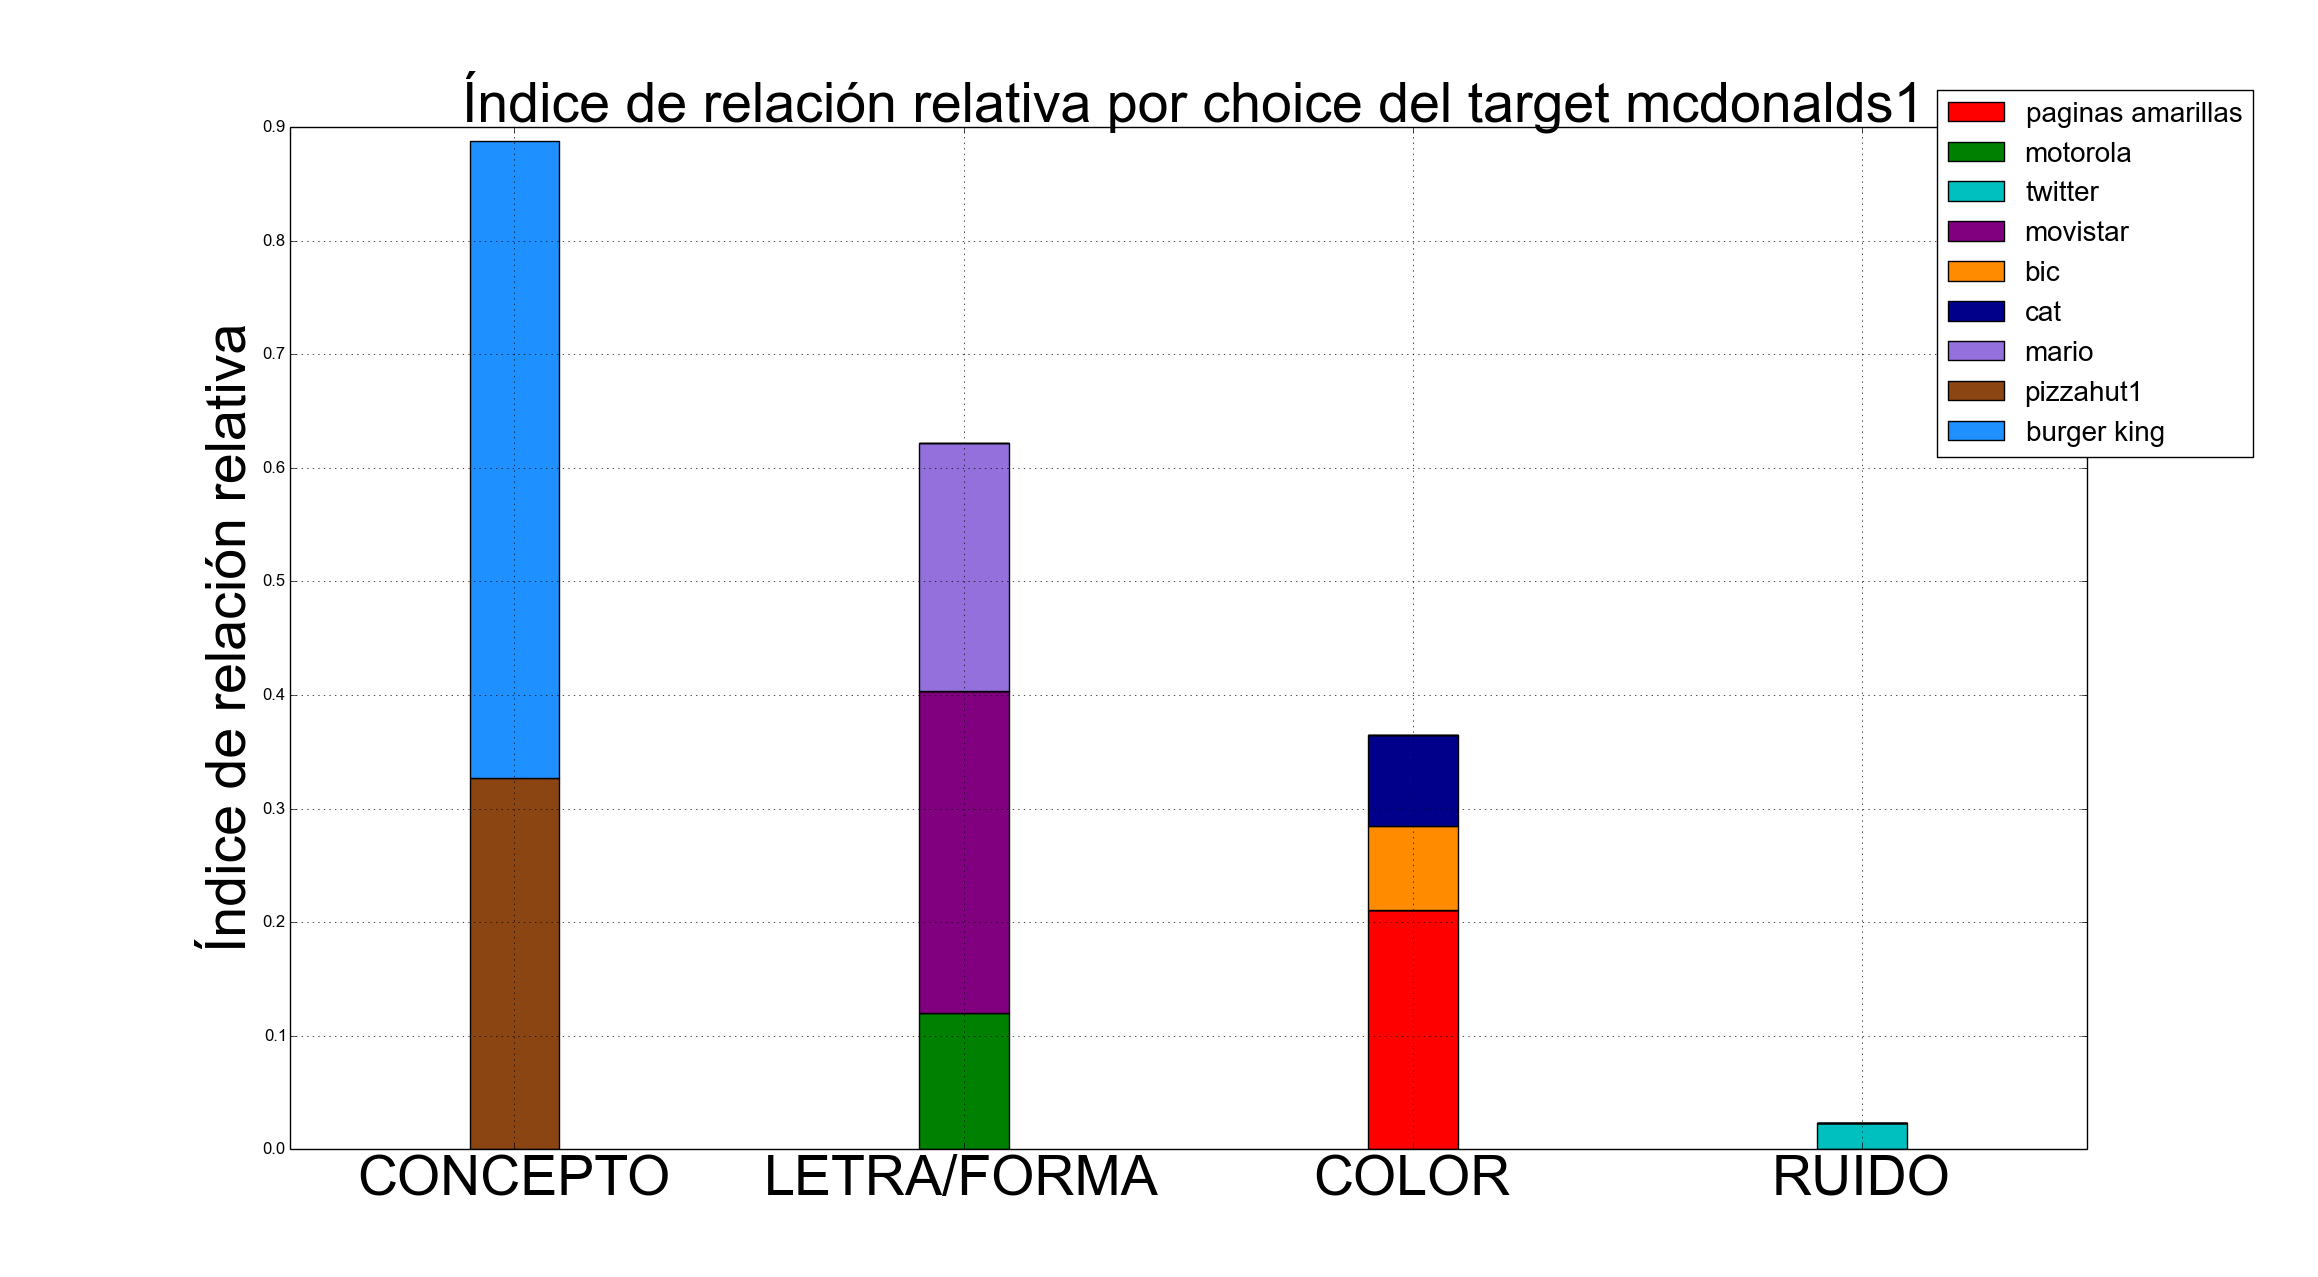
\includegraphics[scale=0.108]{mcdonalds1.png}
	
\includegraphics[scale=0.108]{facebook.png}
  \end{minipage}
  \begin{minipage}[c]{1\textwidth}
	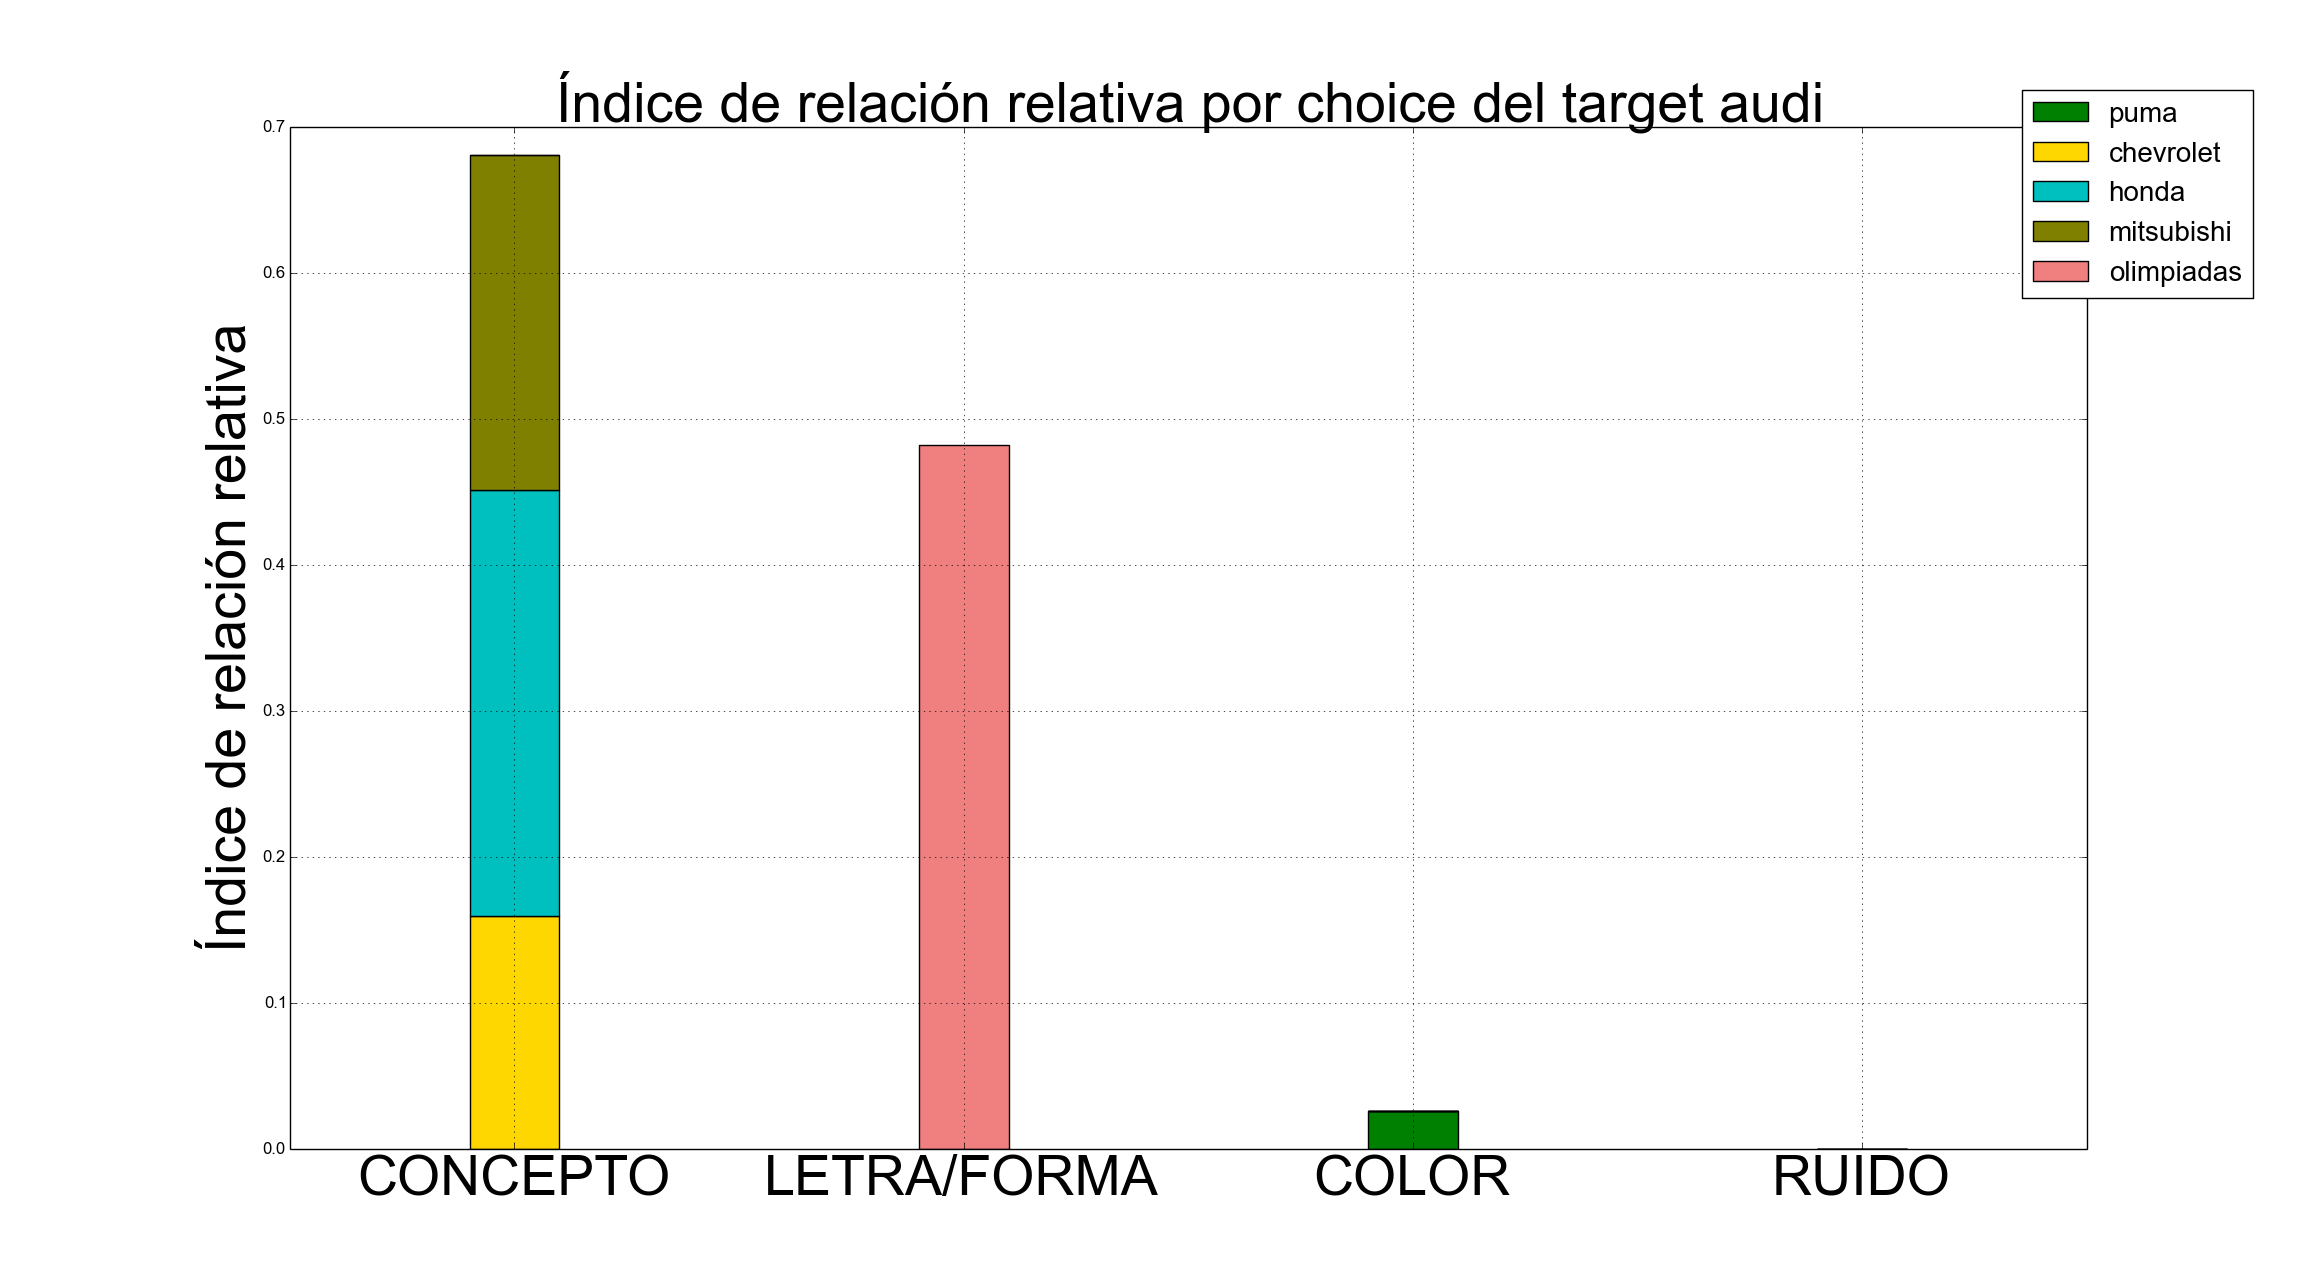
\includegraphics[scale=0.108]{audi.png}
	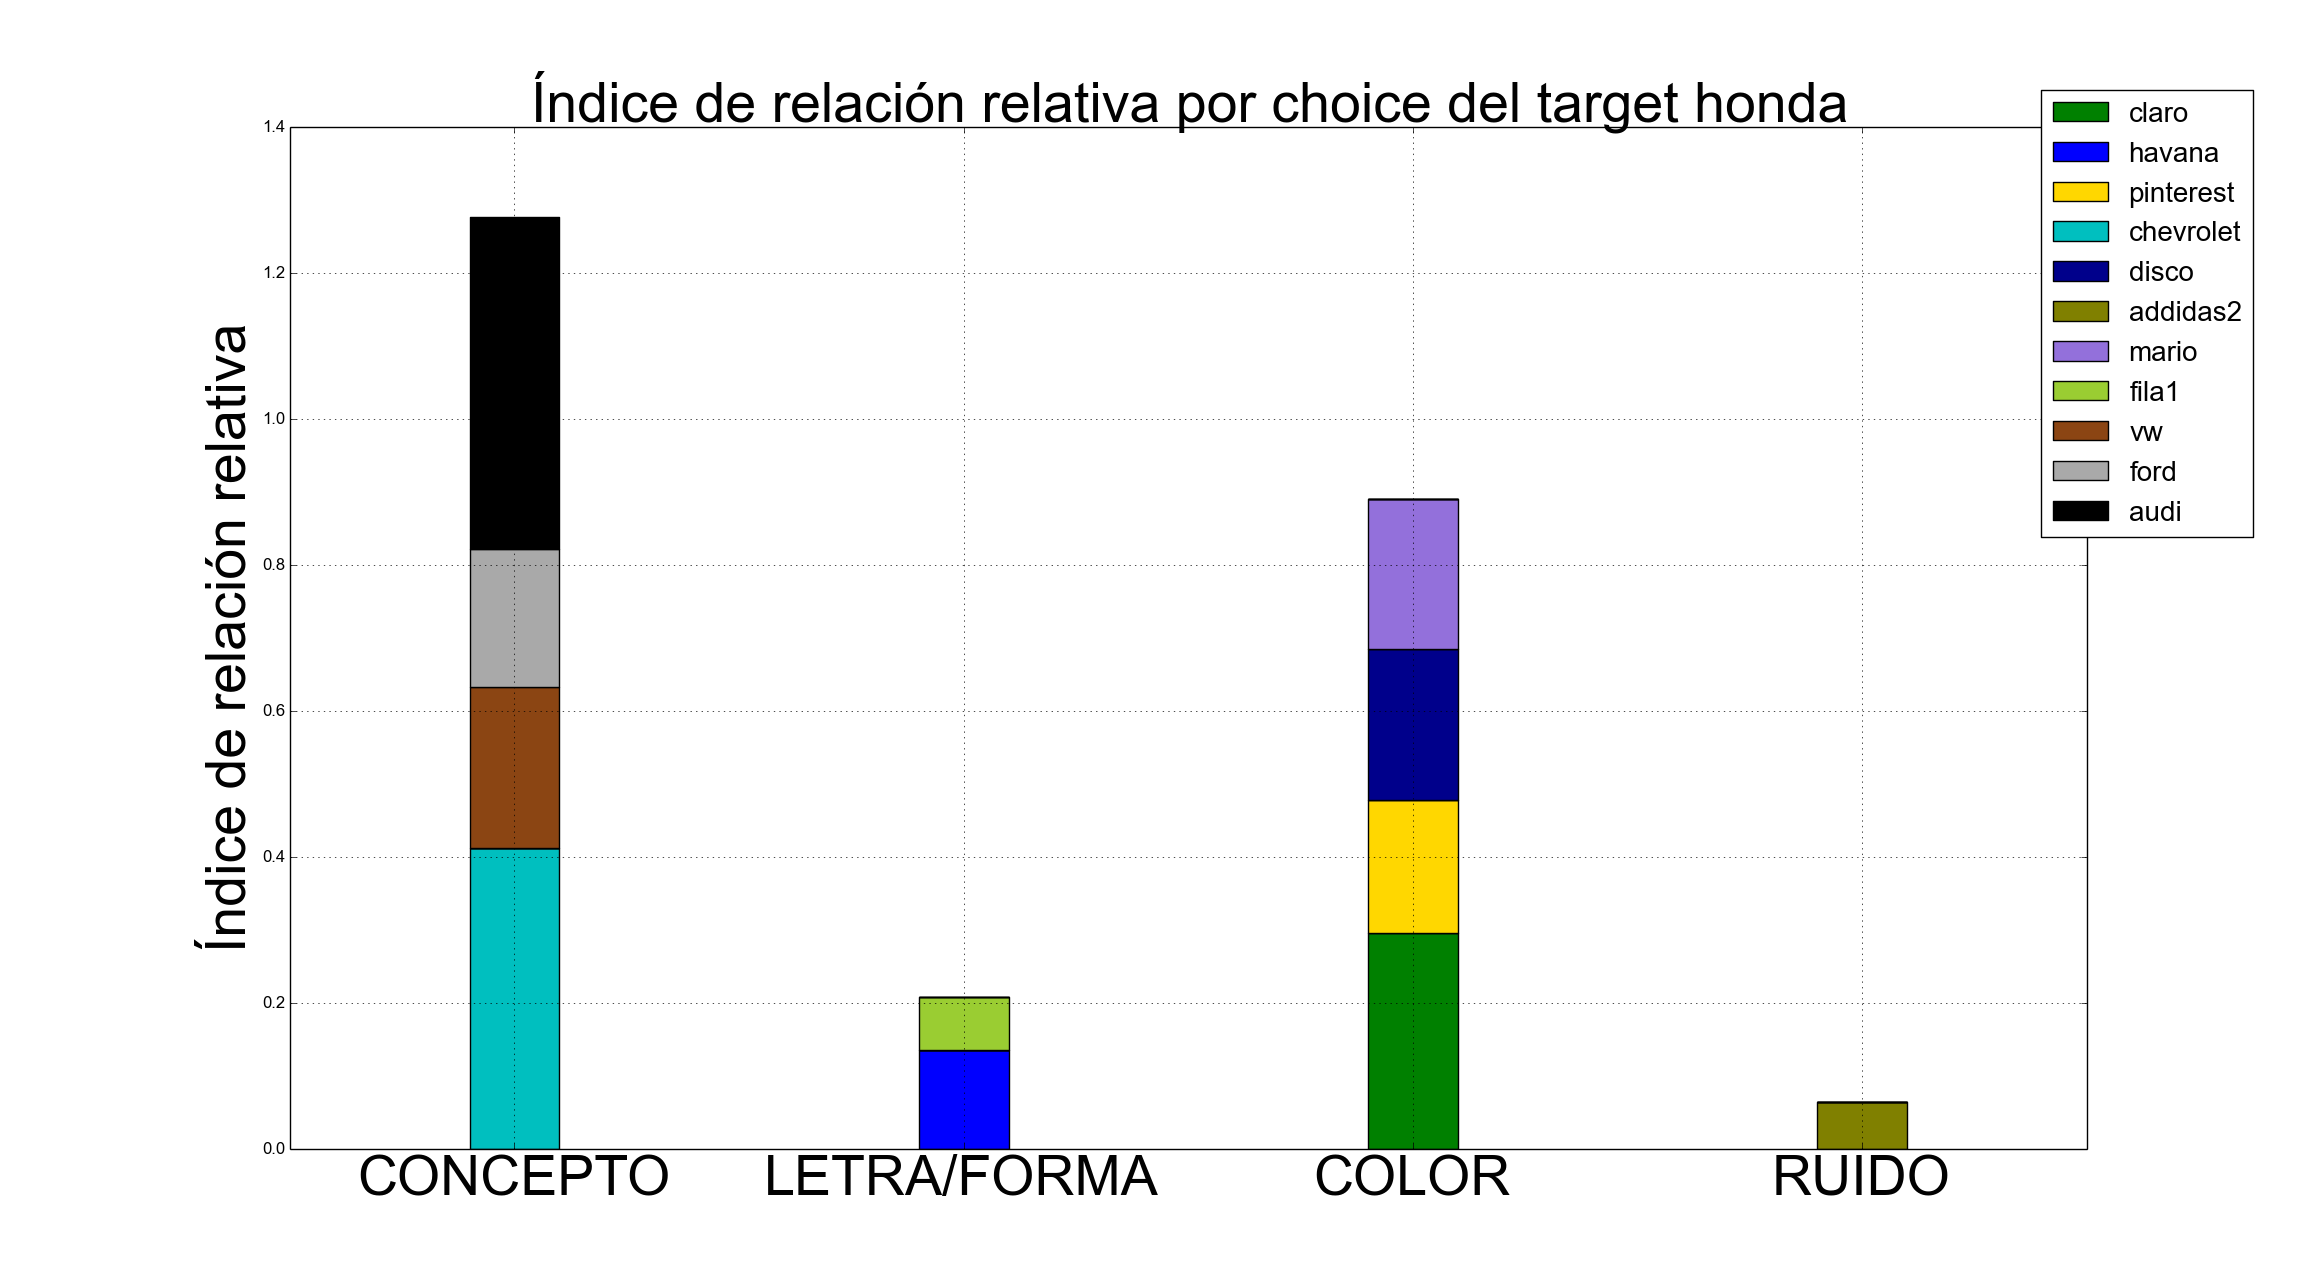
\includegraphics[scale=0.108]{honda.png}
  \end{minipage}
\end{figure}
\end{frame}

\begin{frame}
\begin{figure}[h]
 \centering
  \begin{minipage}[c]{1\textwidth}
	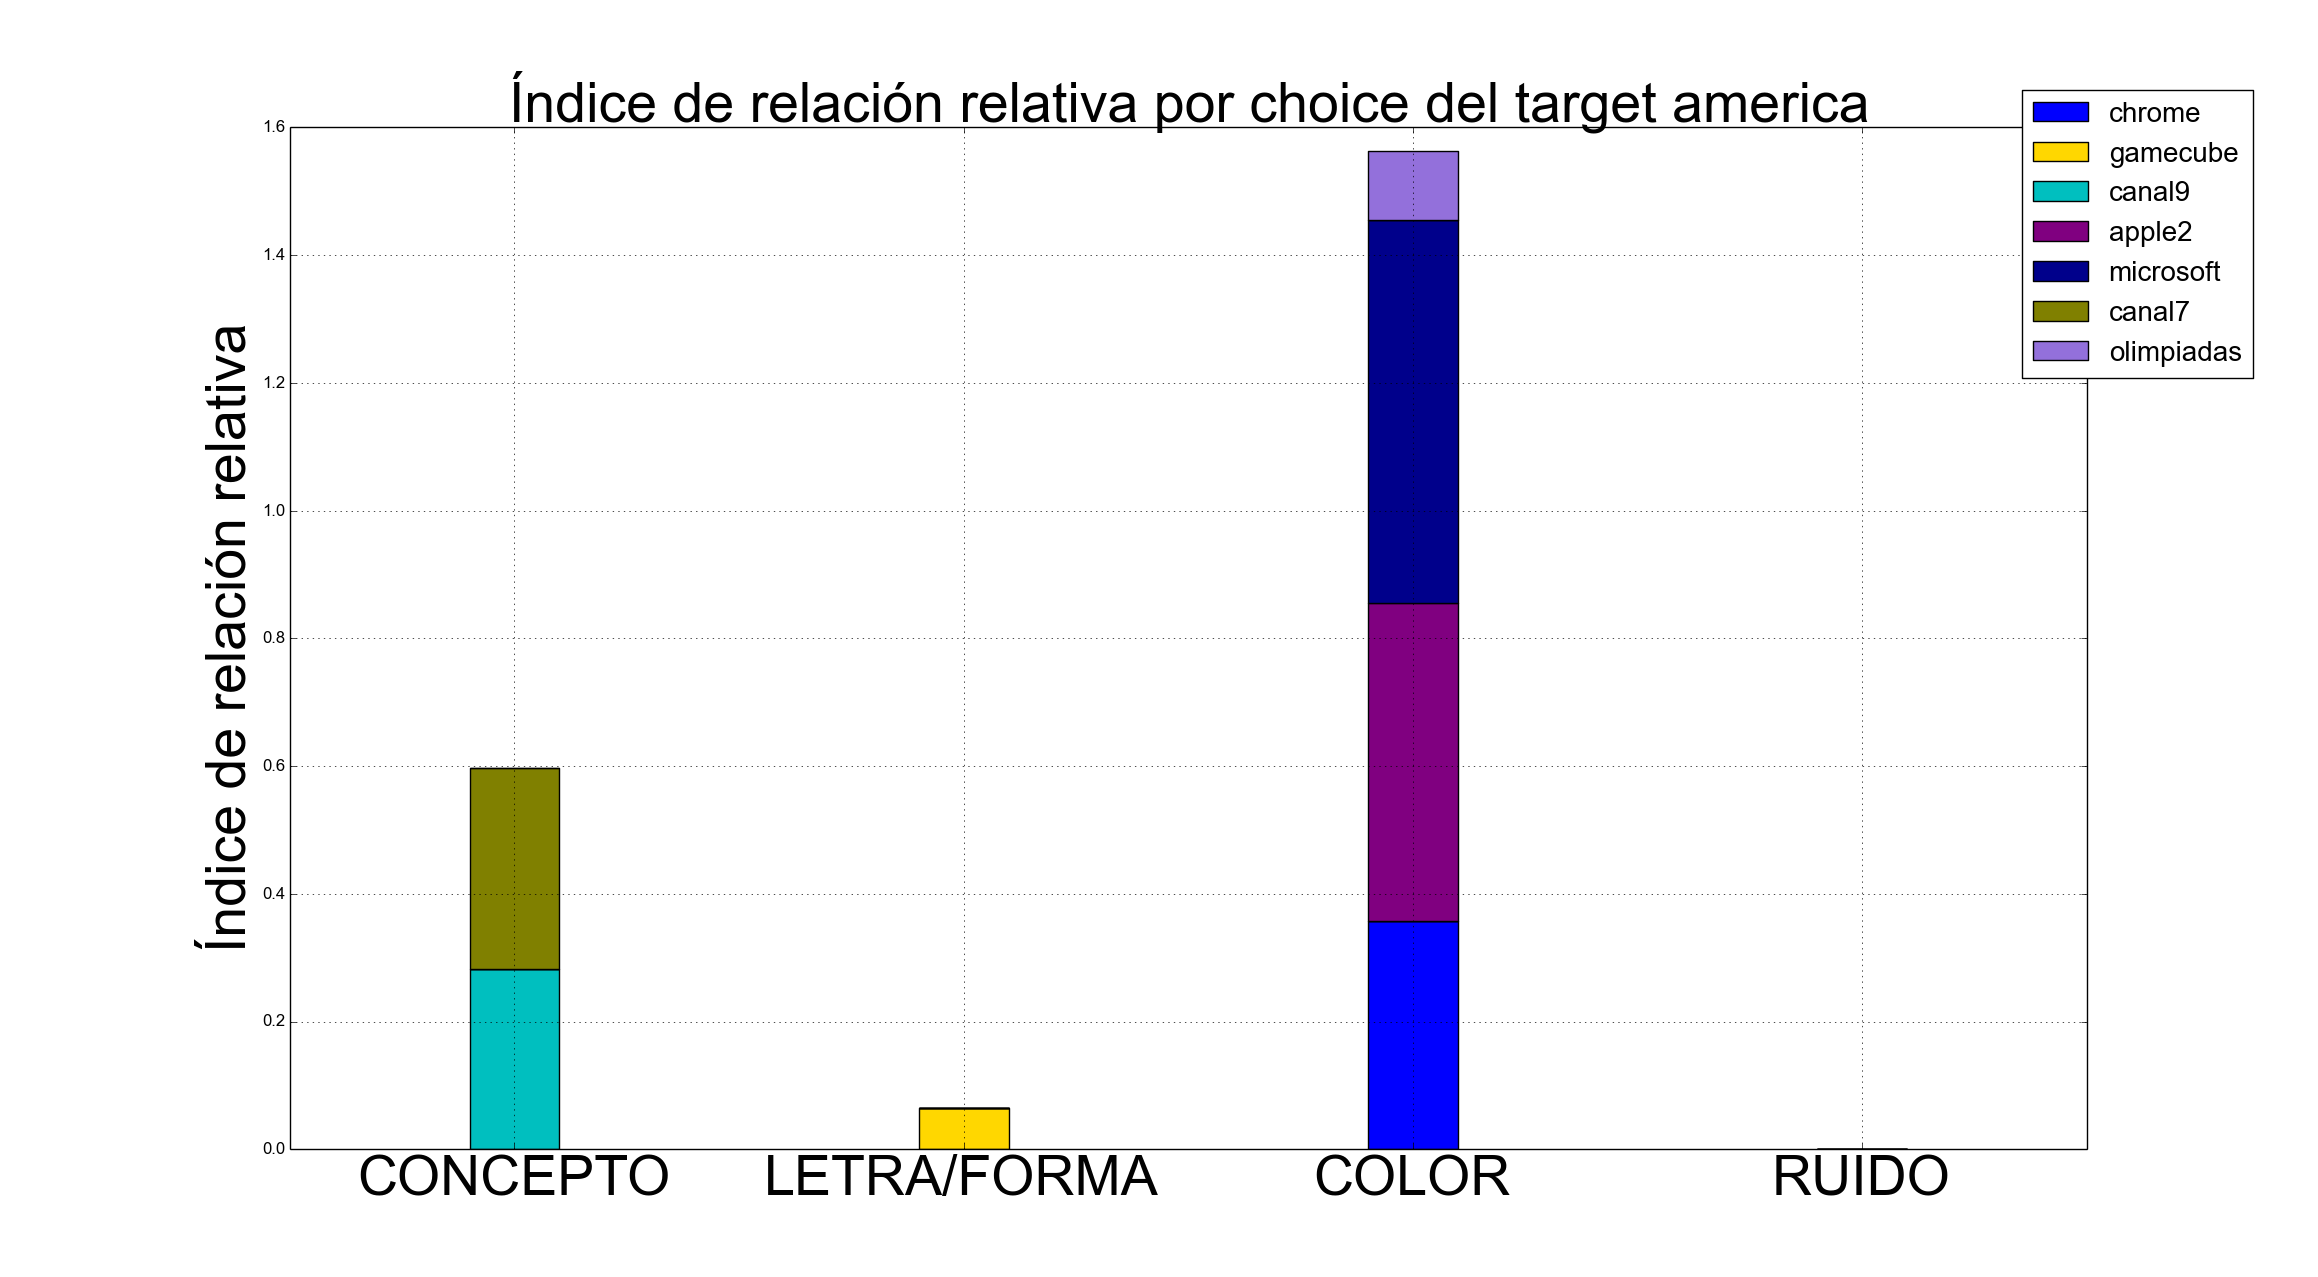
\includegraphics[scale=0.108]{america.png}
	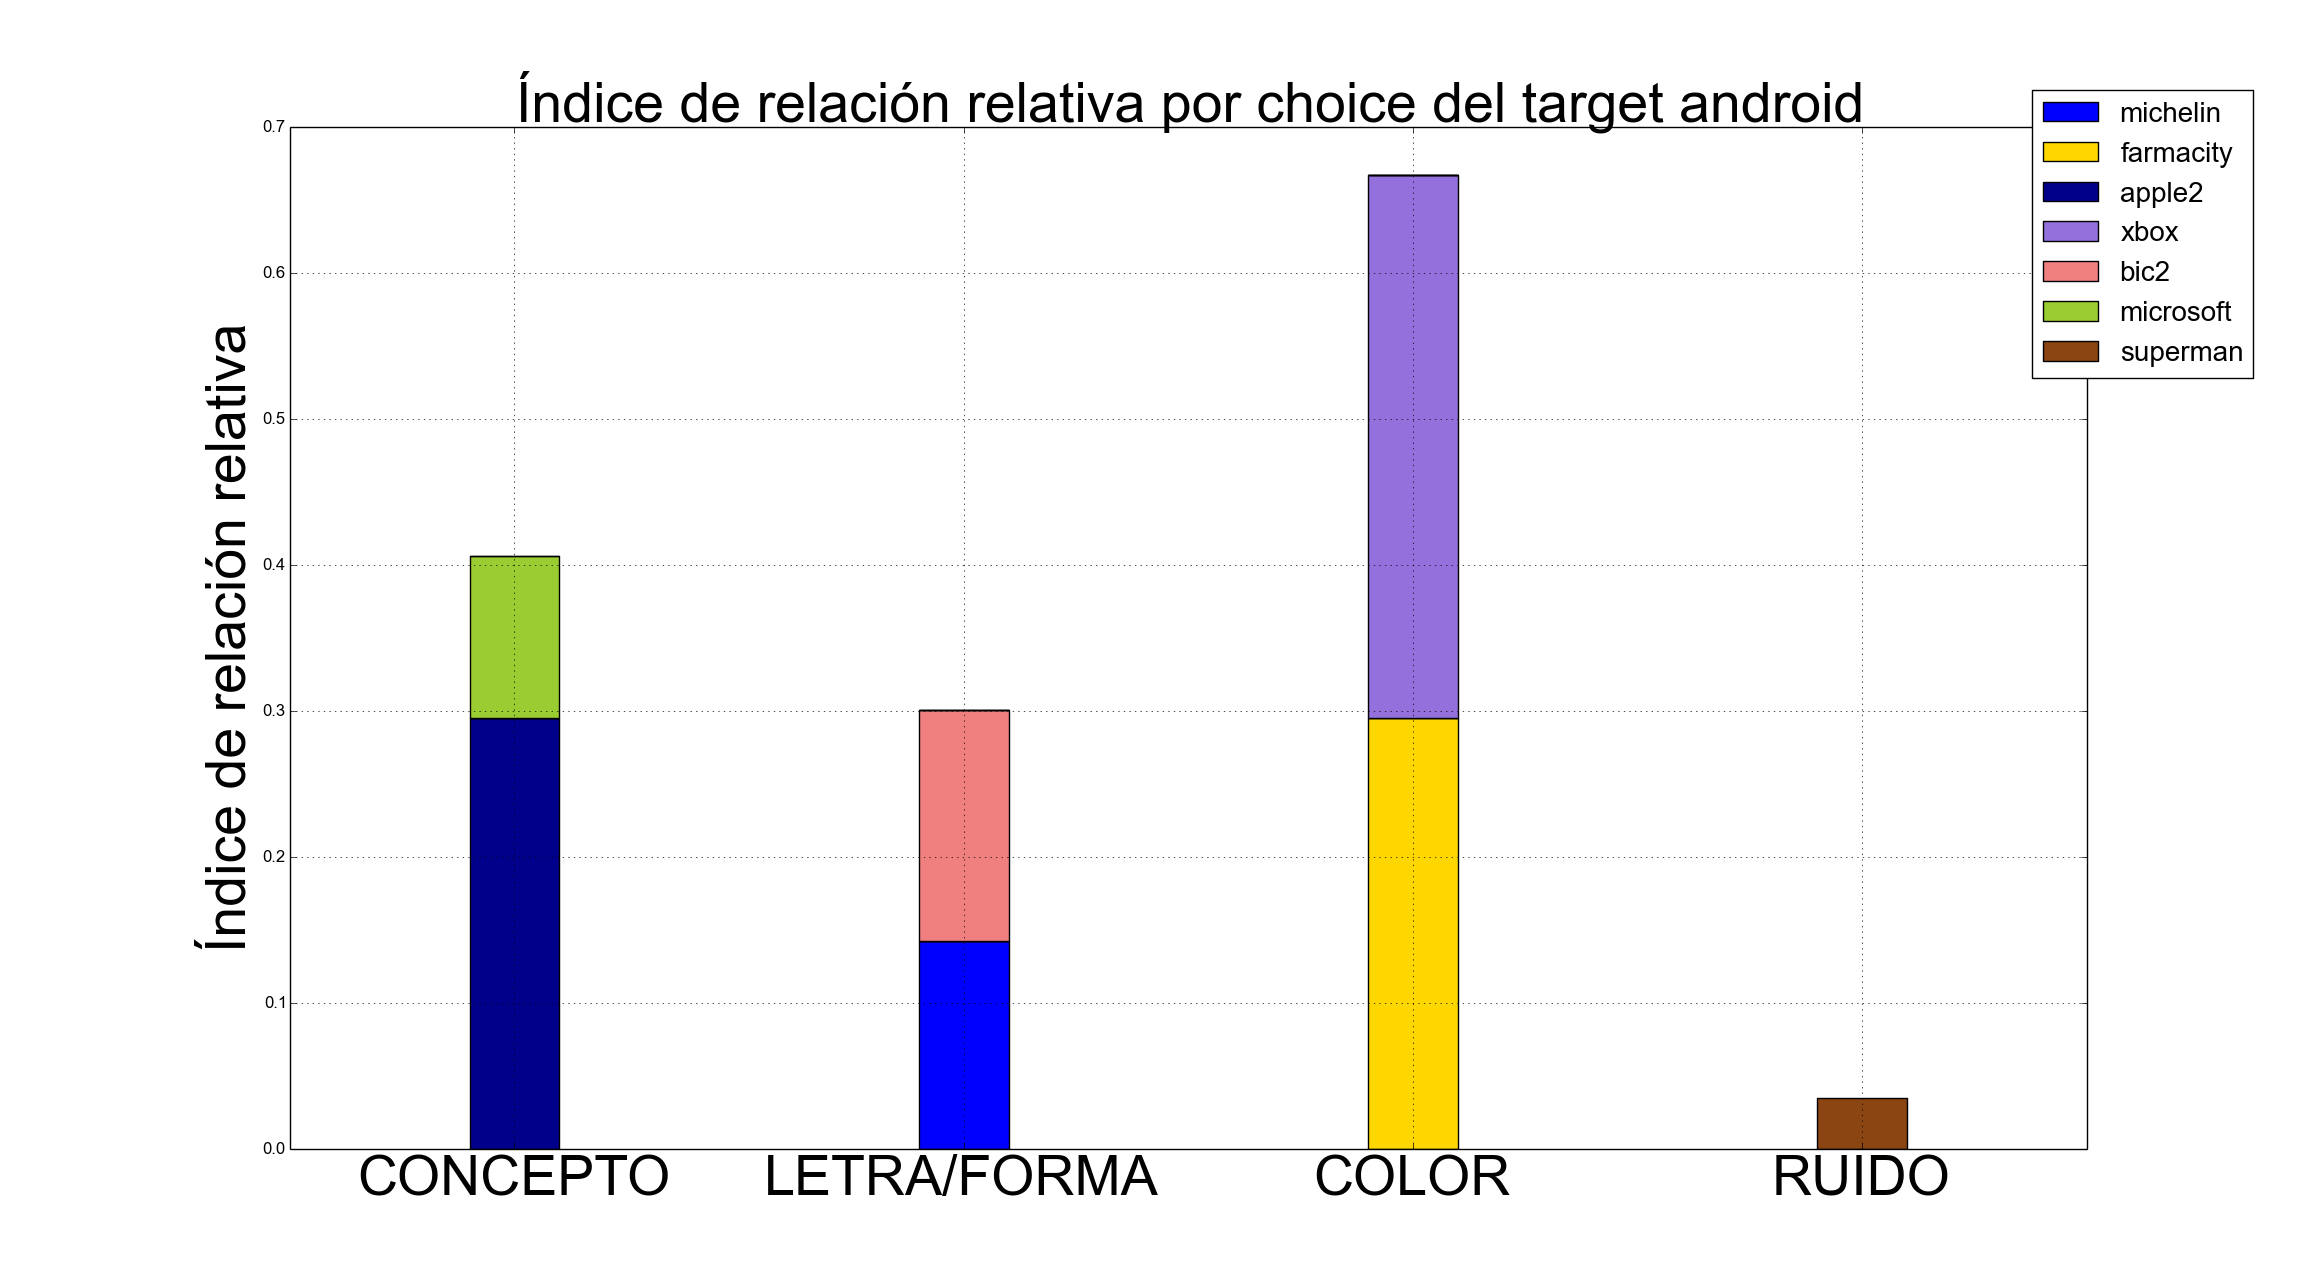
\includegraphics[scale=0.108]{android.png}
  \end{minipage}
  \begin{minipage}[c]{1\textwidth}
	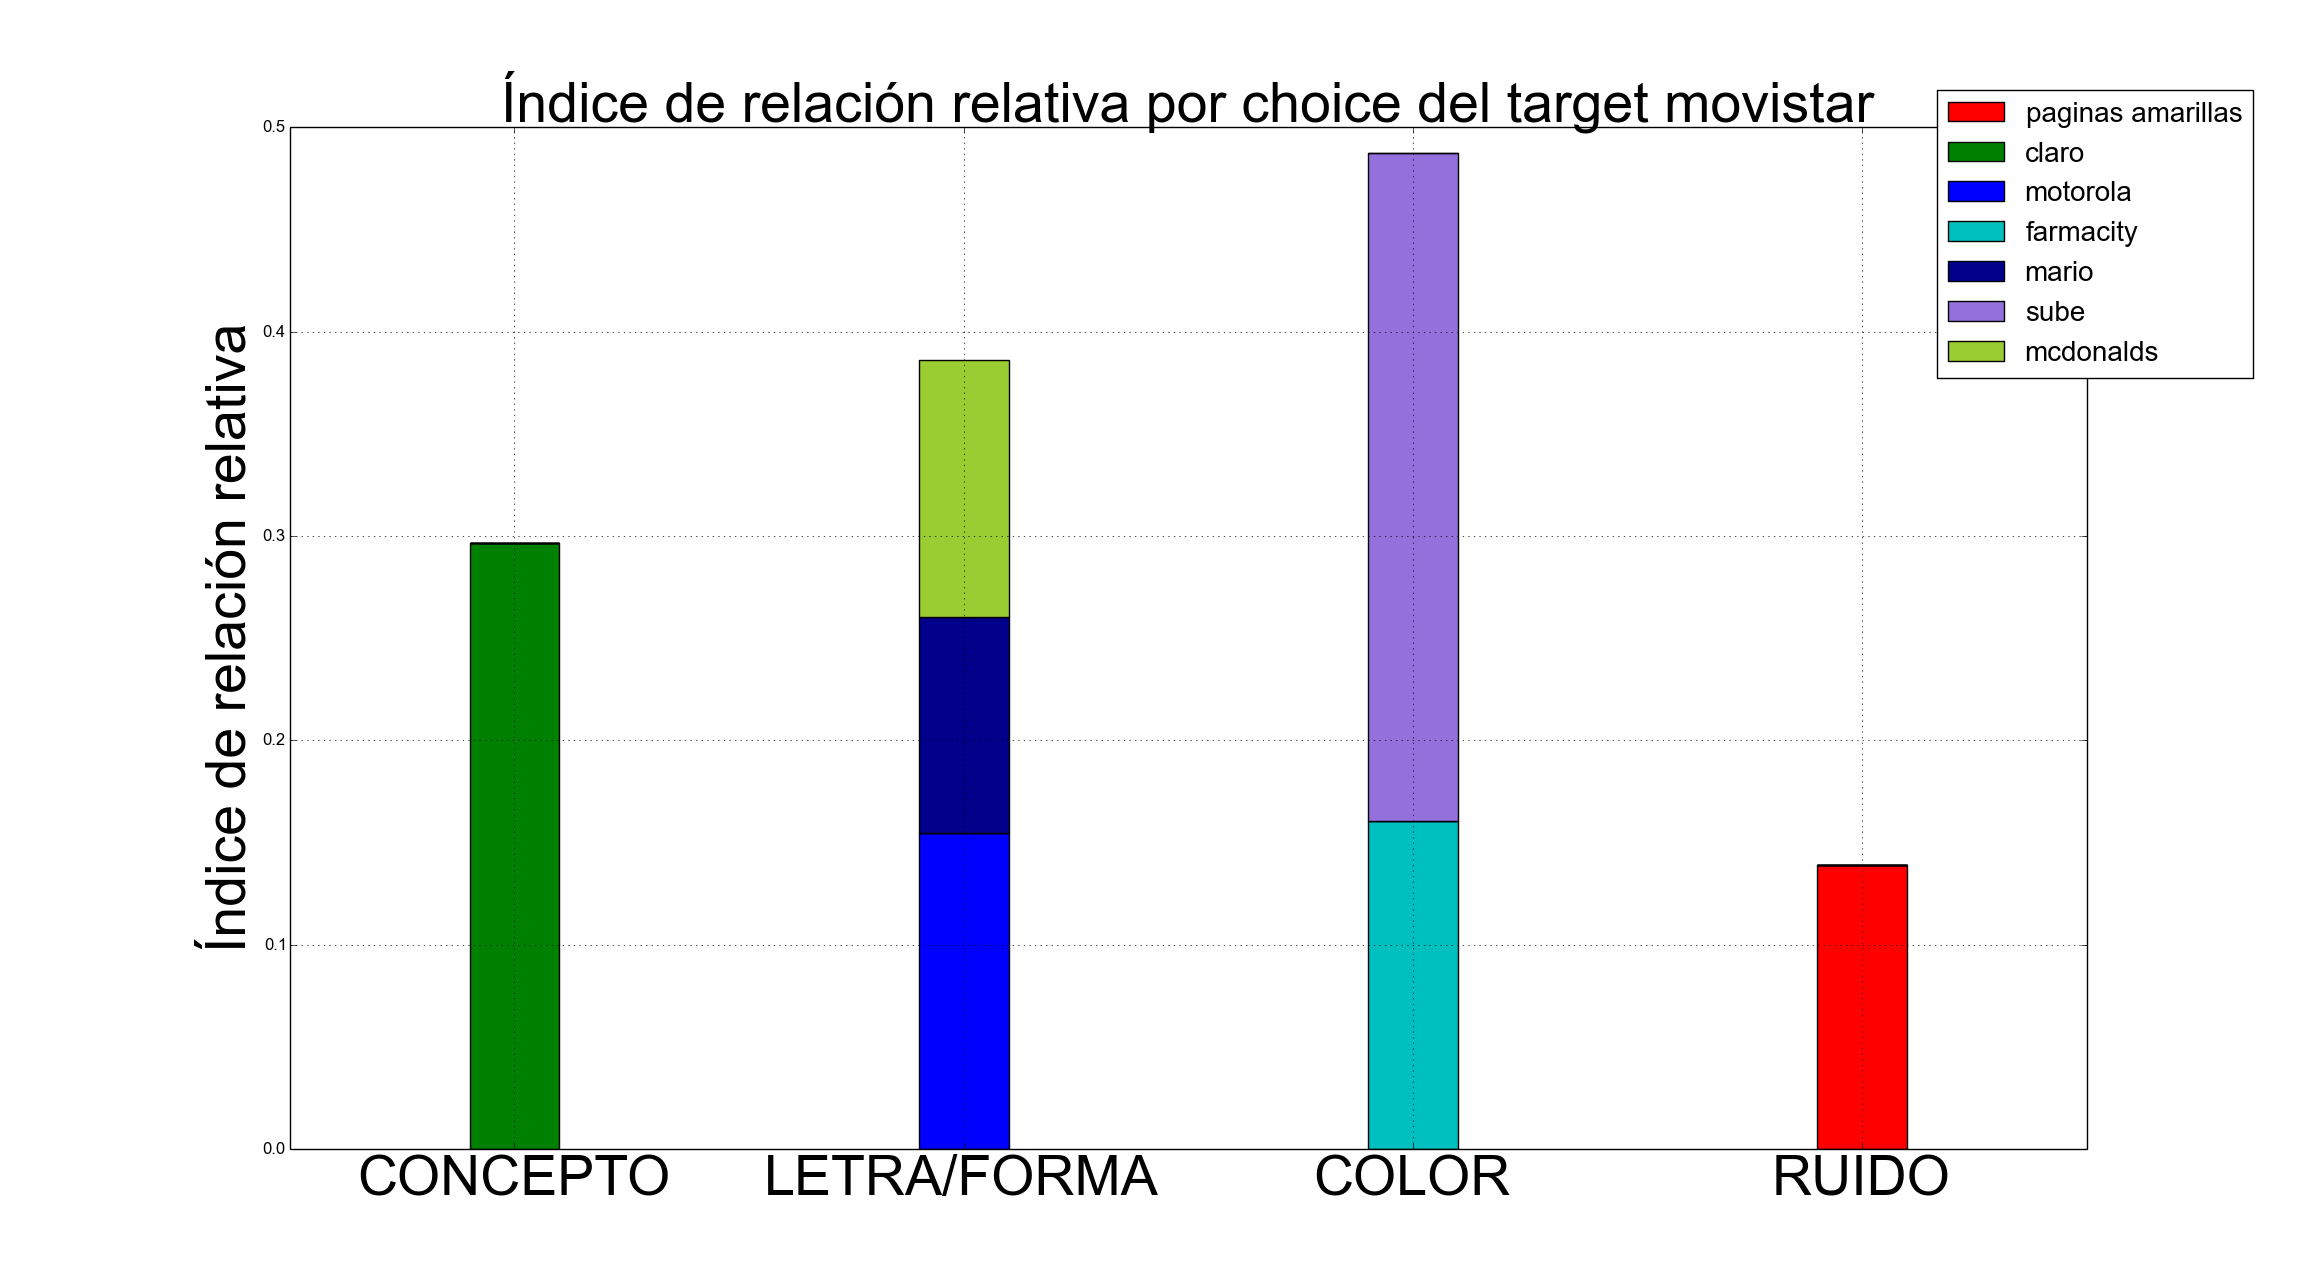
\includegraphics[scale=0.108]{movistar.png}
	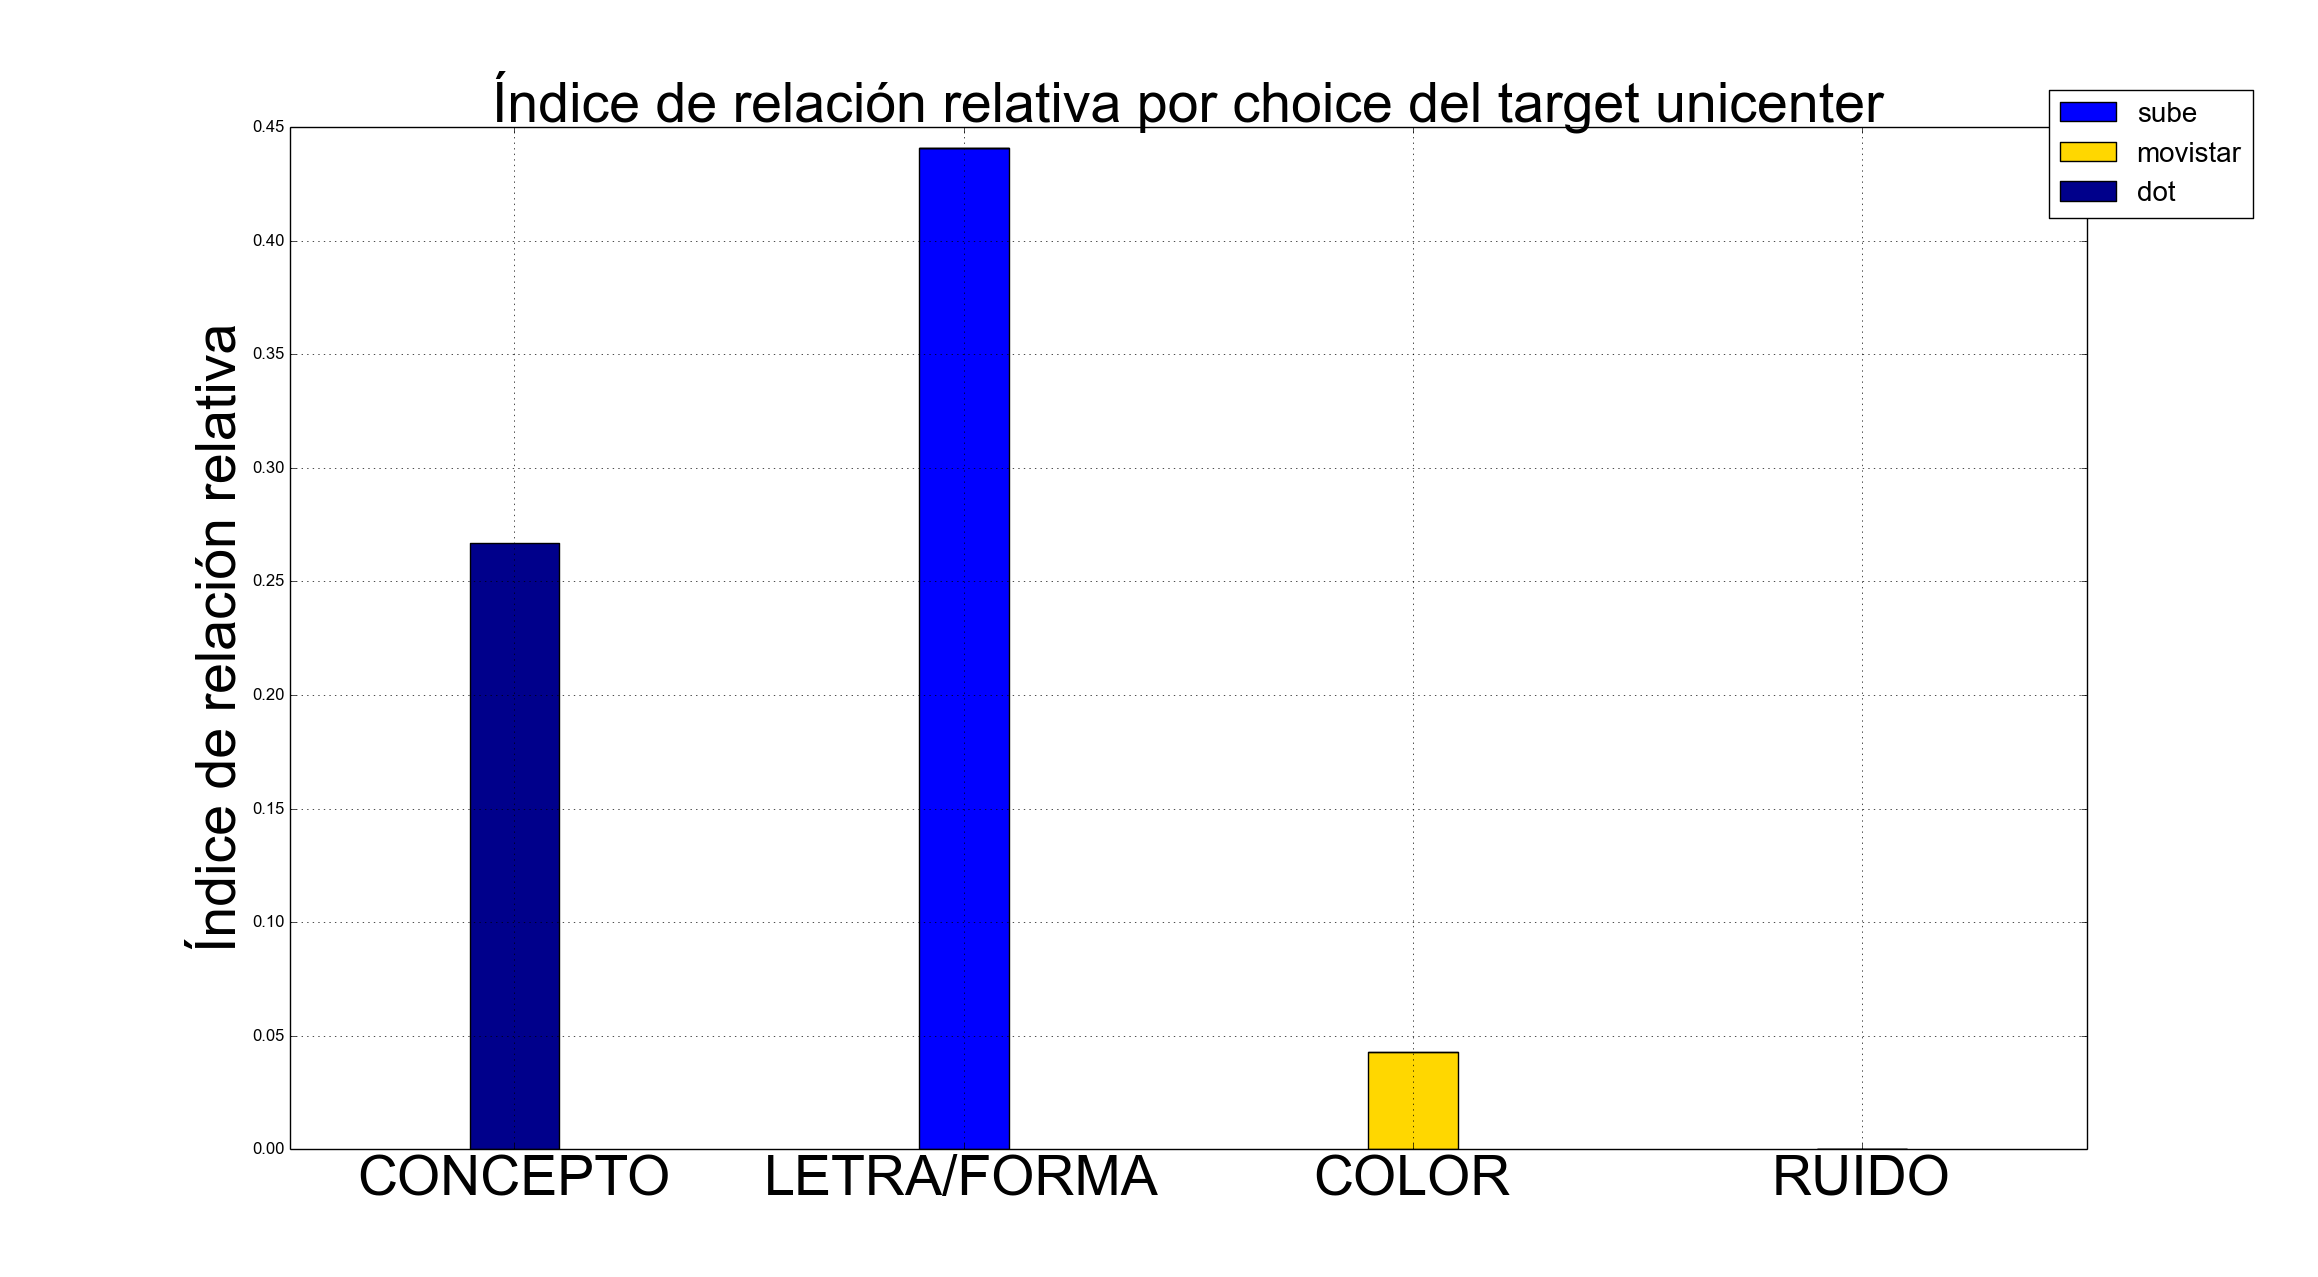
\includegraphics[scale=0.108]{unicenter.png}
  \end{minipage}
\end{figure}
\end{frame}

\begin{frame}
\begin{figure}[h]
 \centering
  \begin{minipage}[c]{1\textwidth}
	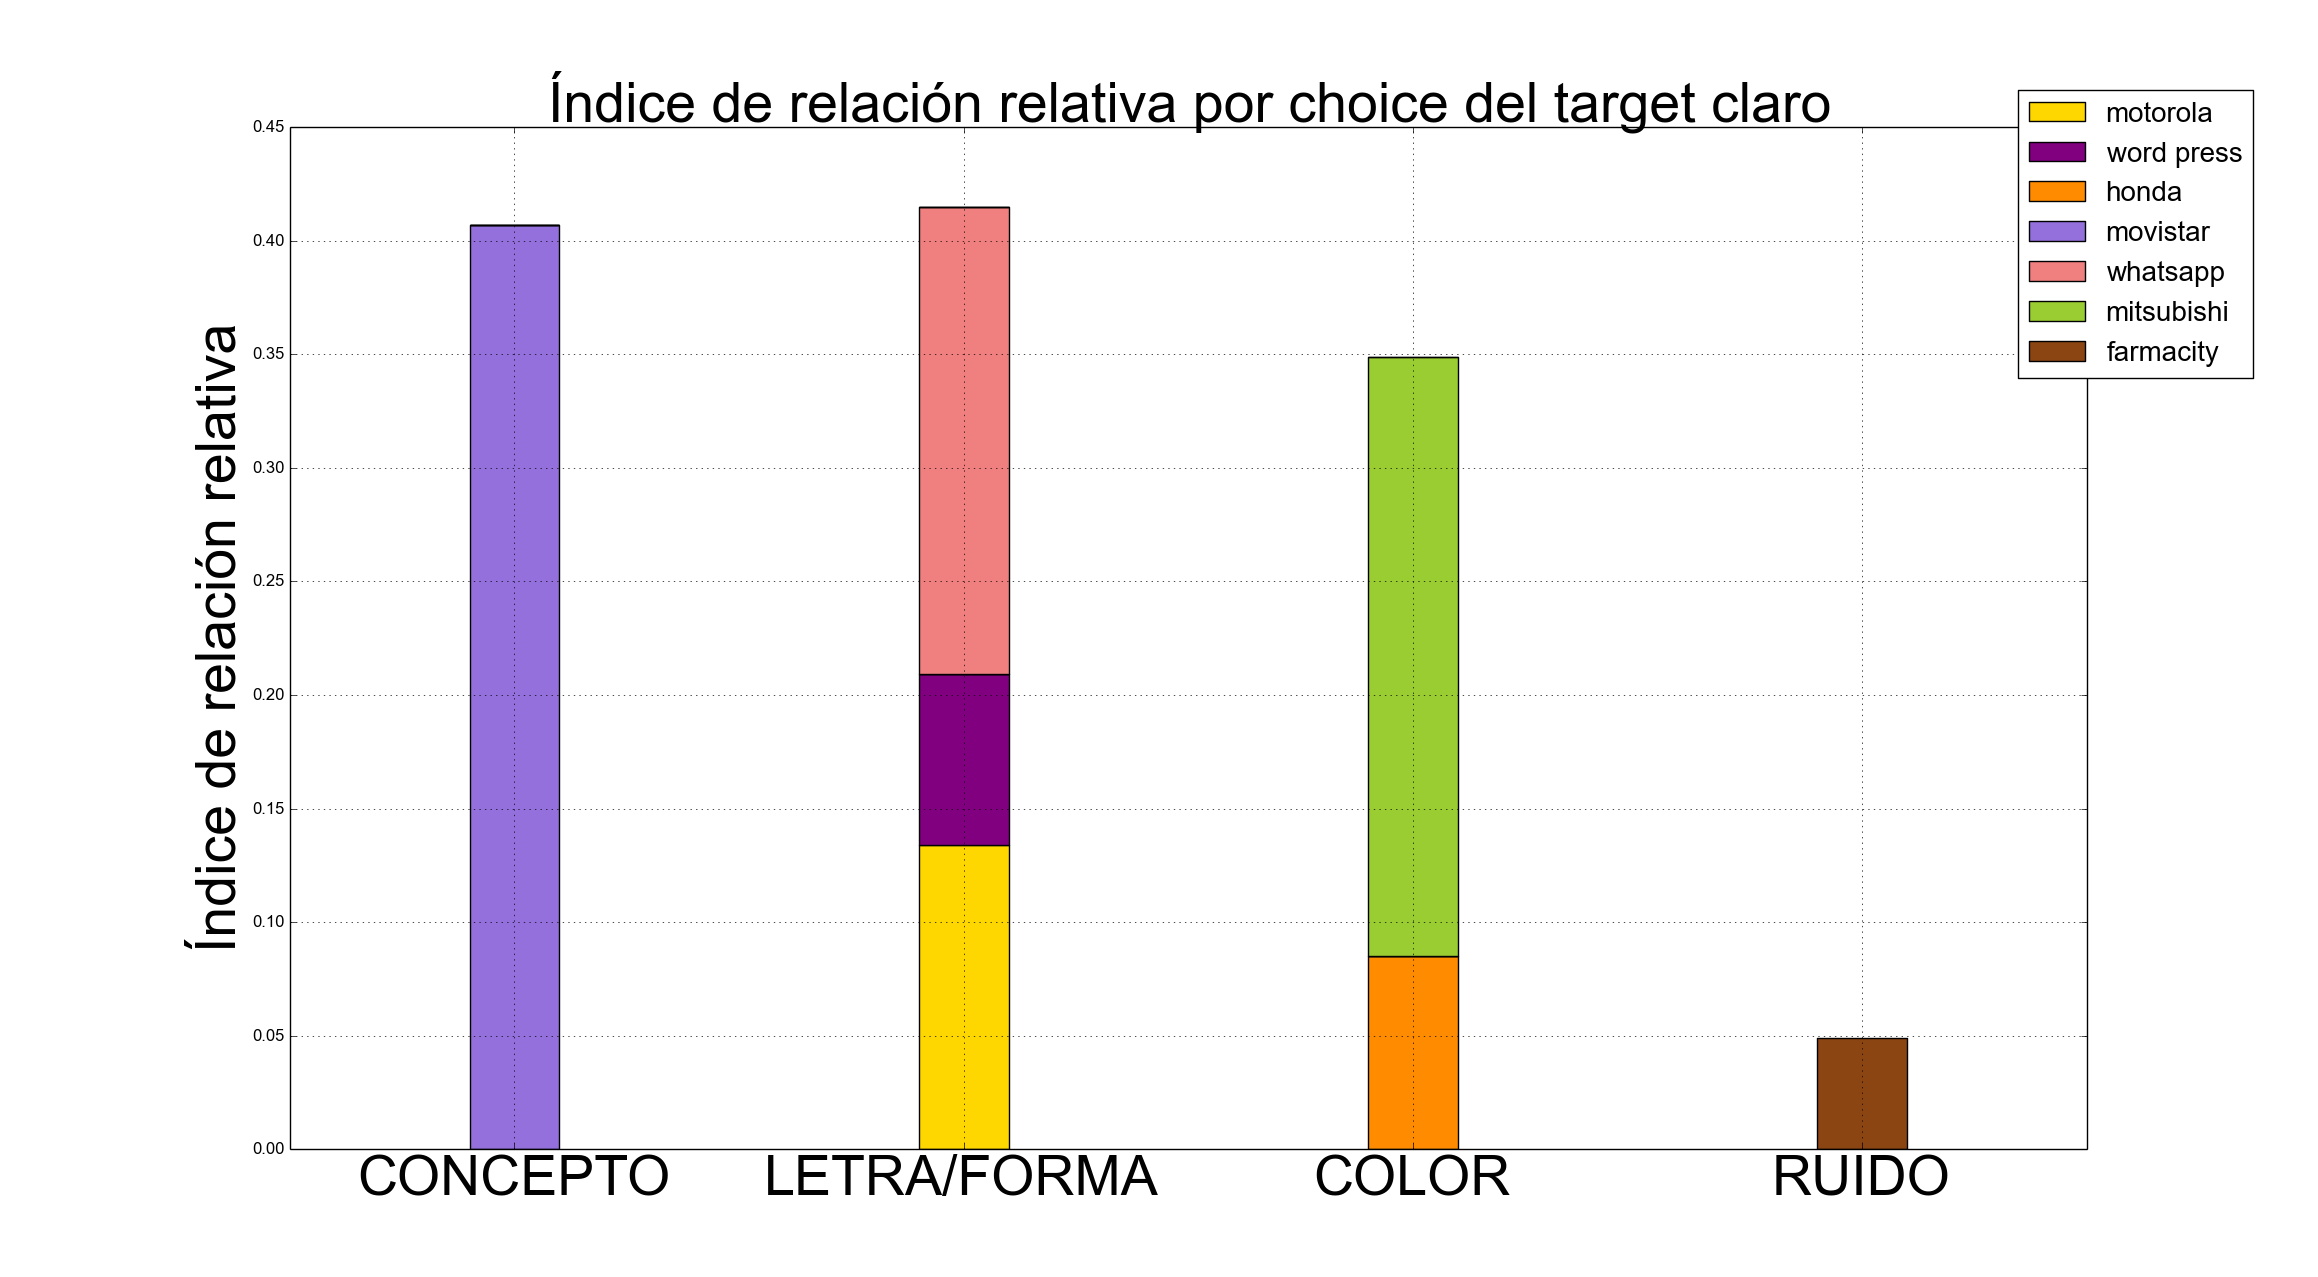
\includegraphics[scale=0.108]{claro.png}
	
\includegraphics[scale=0.108]{farmacity.png}
  \end{minipage}
  \begin{minipage}[c]{1\textwidth}
	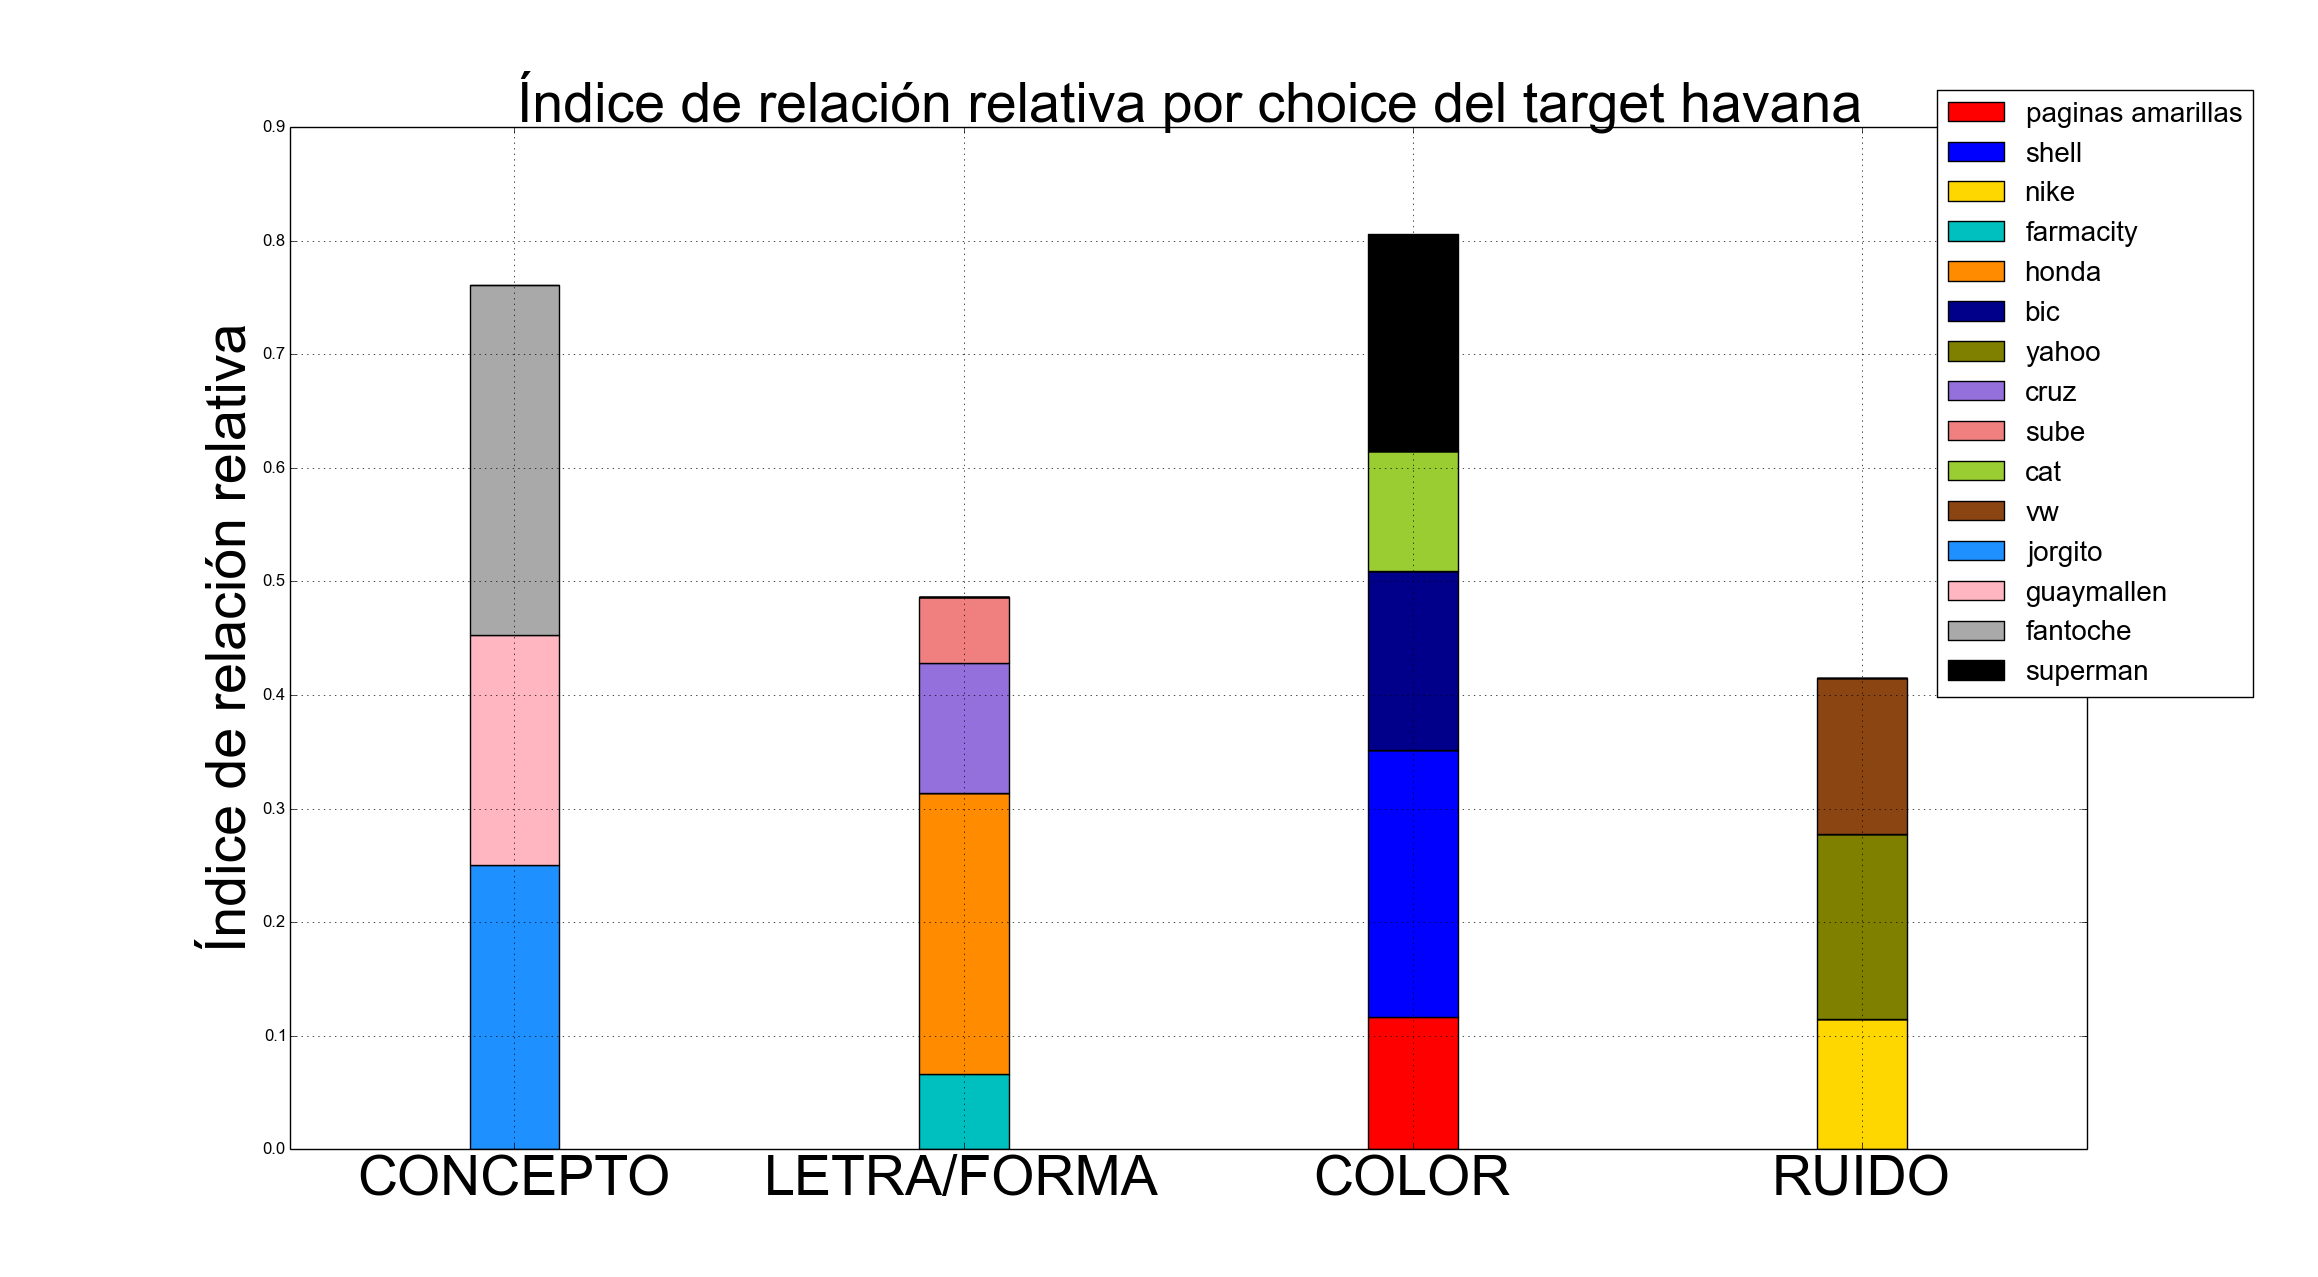
\includegraphics[scale=0.108]{havana.png}
  \end{minipage}
\end{figure}
\end{frame}

\begin{frame}
\begin{figure}[h]
 \centering
  \begin{minipage}[c]{1\textwidth}
	\centering	
	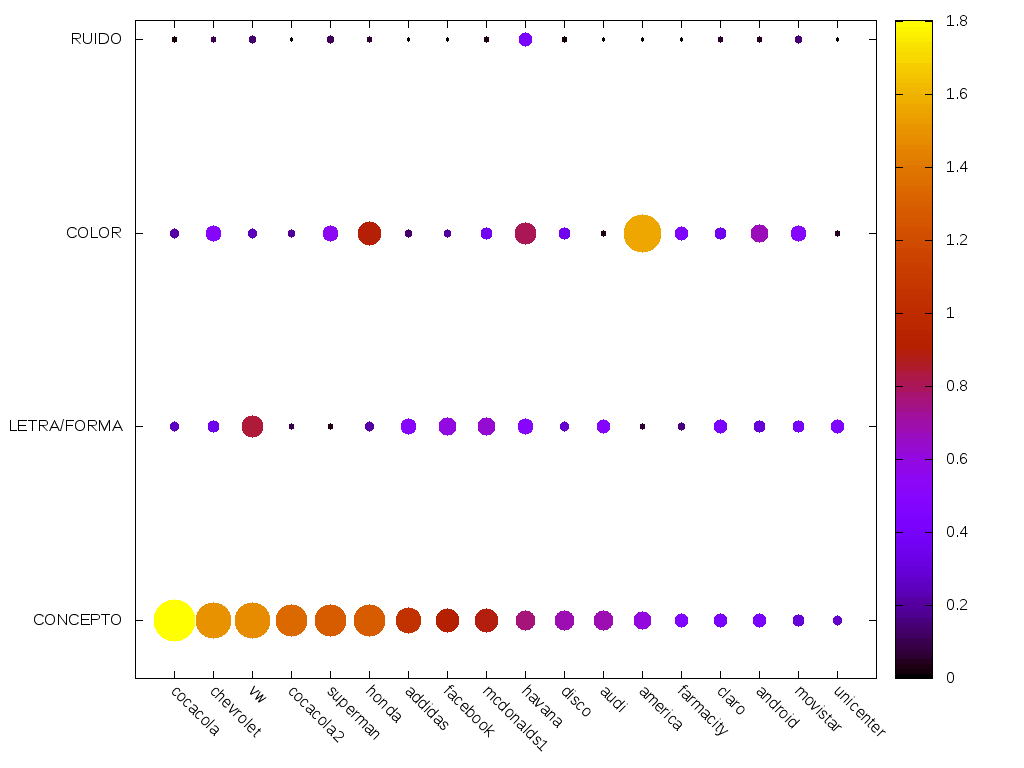
\includegraphics[scale=0.4]{target_ir.png}
  \end{minipage}
\end{figure}
\end{frame}

\begin{frame}
\begin{figure}[h]
 \centering
  \begin{minipage}[c]{1\textwidth}
	\centering	
	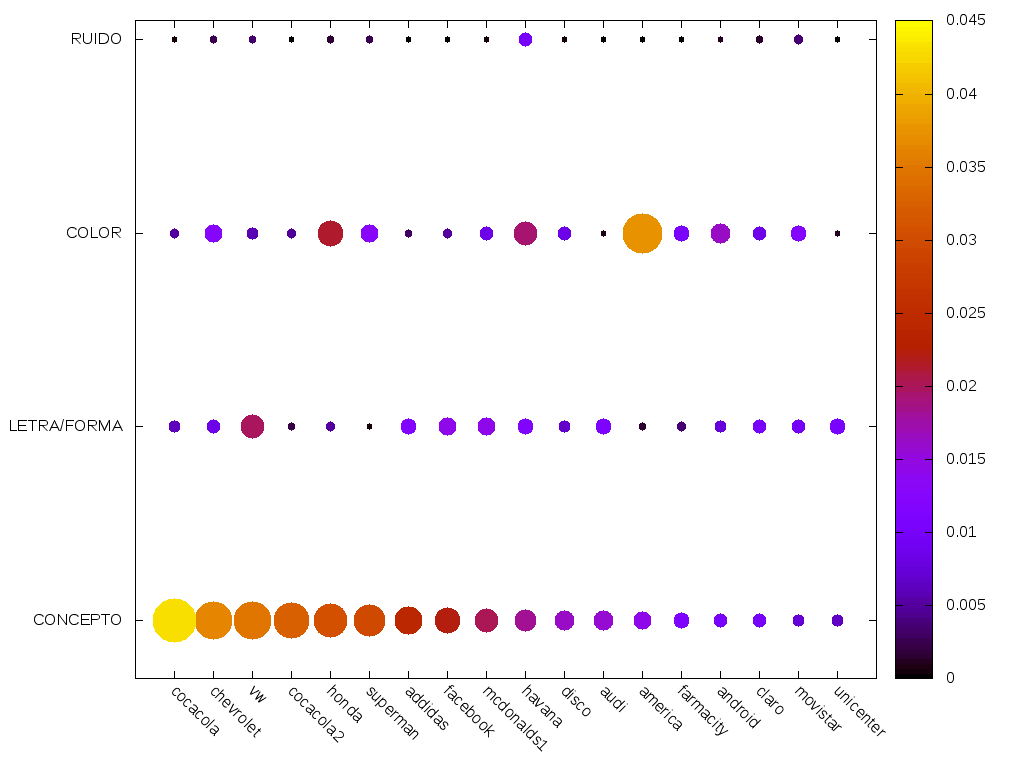
\includegraphics[scale=0.4]{target_irr.png}
  \end{minipage}
\end{figure}
\end{frame}

\subsection{Random Trials}

\begin{frame}
\begin{figure}[h]
 \centering
  \begin{minipage}[c]{1\textwidth}
	\centering	
	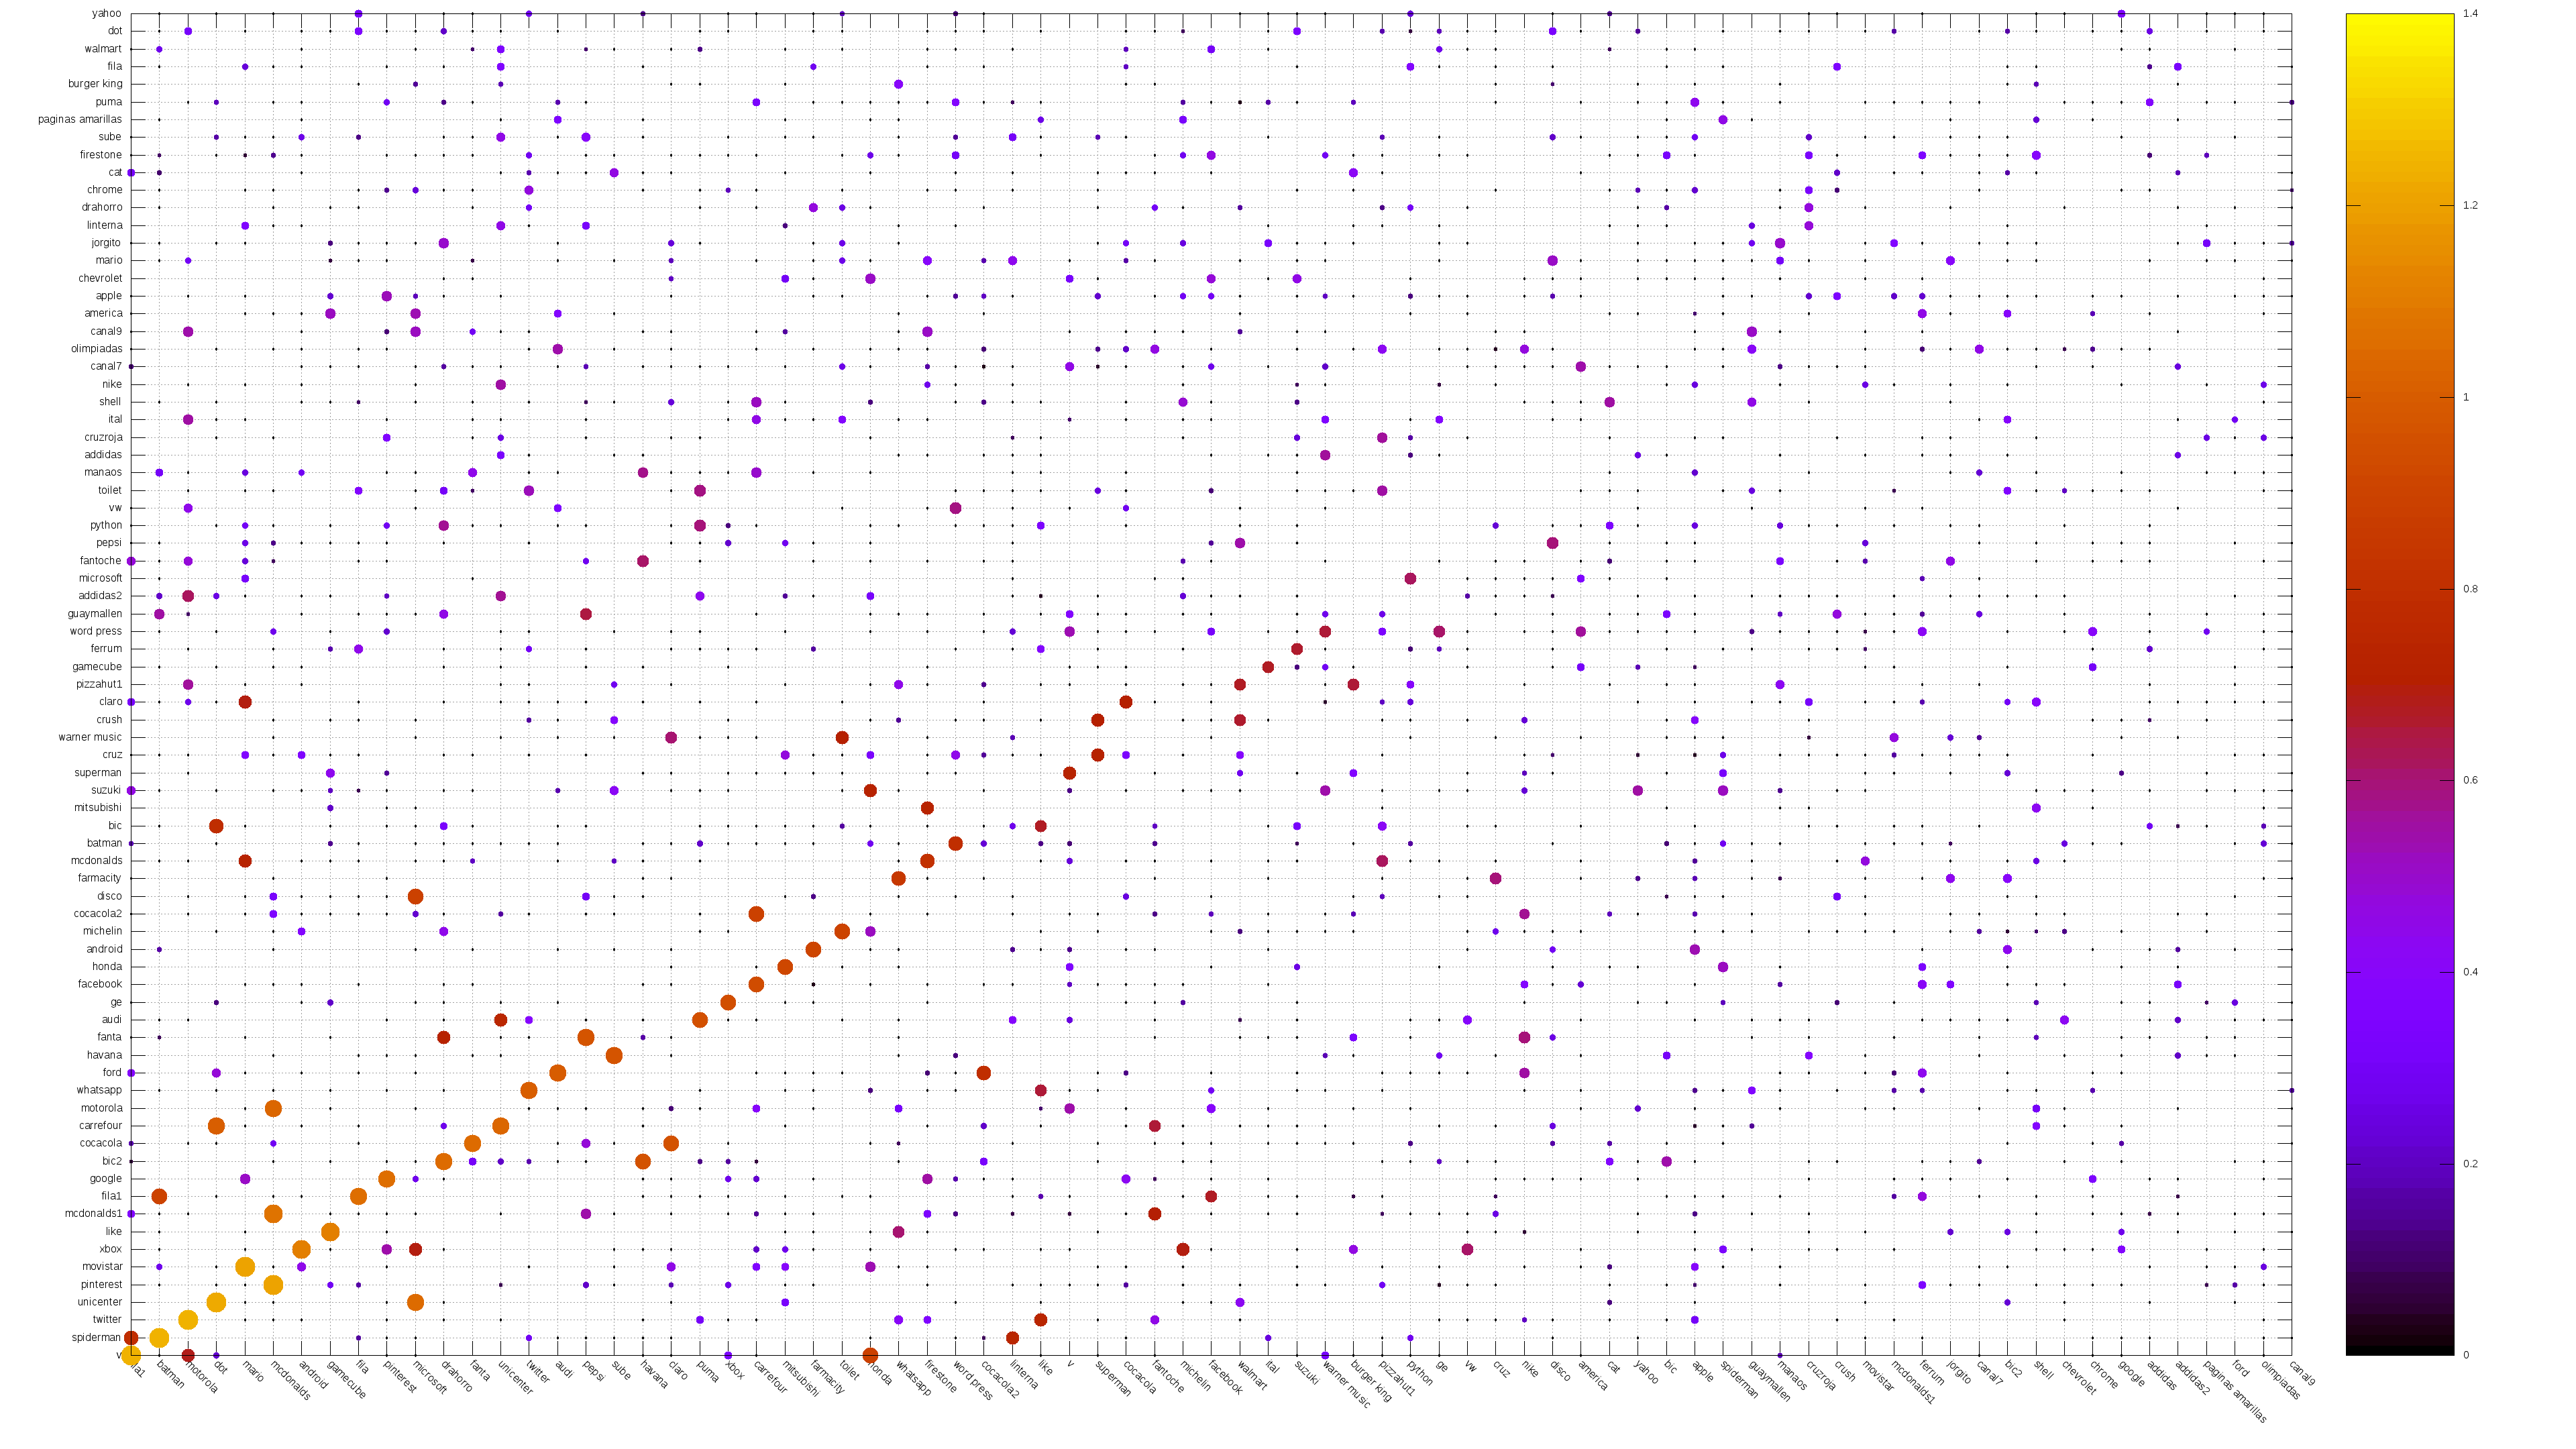
\includegraphics[scale=0.13]{random.png}
  \end{minipage}
\end{figure}
\end{frame}

\begin{frame}
\begin{figure}[h]
 \centering
  \begin{minipage}[c]{1\textwidth}
	\centering	
	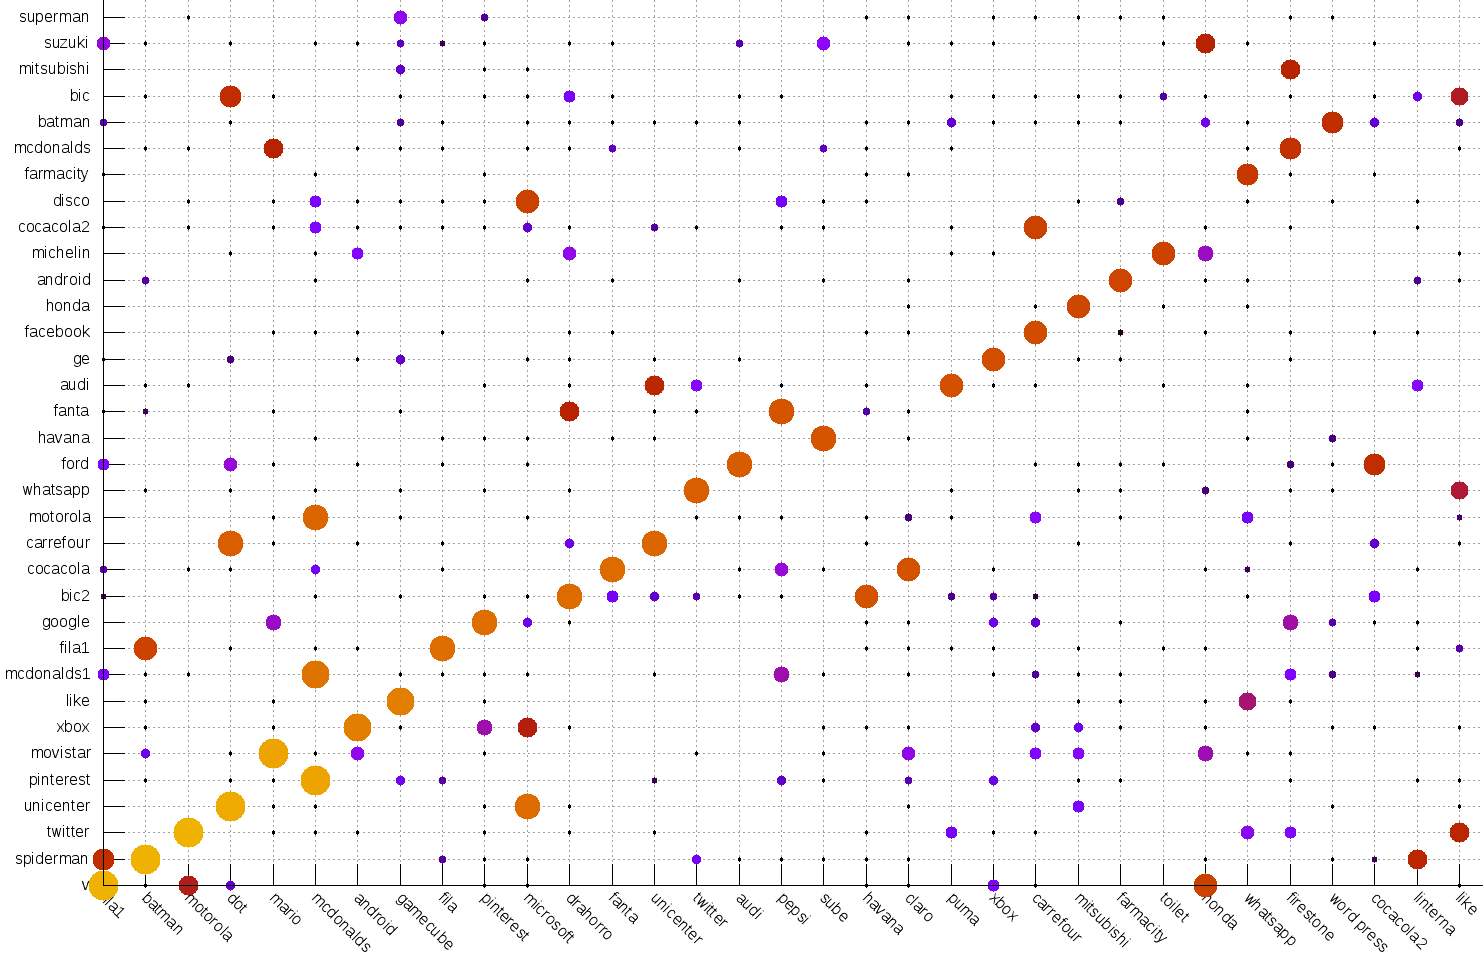
\includegraphics[scale=0.32]{randomx.png}
  \end{minipage}
\end{figure}
\end{frame}

\subsection{Tiempo de respuesta}

\begin{frame}
\begin{figure}[h]
 \centering
  \begin{minipage}[c]{1\textwidth}
	\centering	
	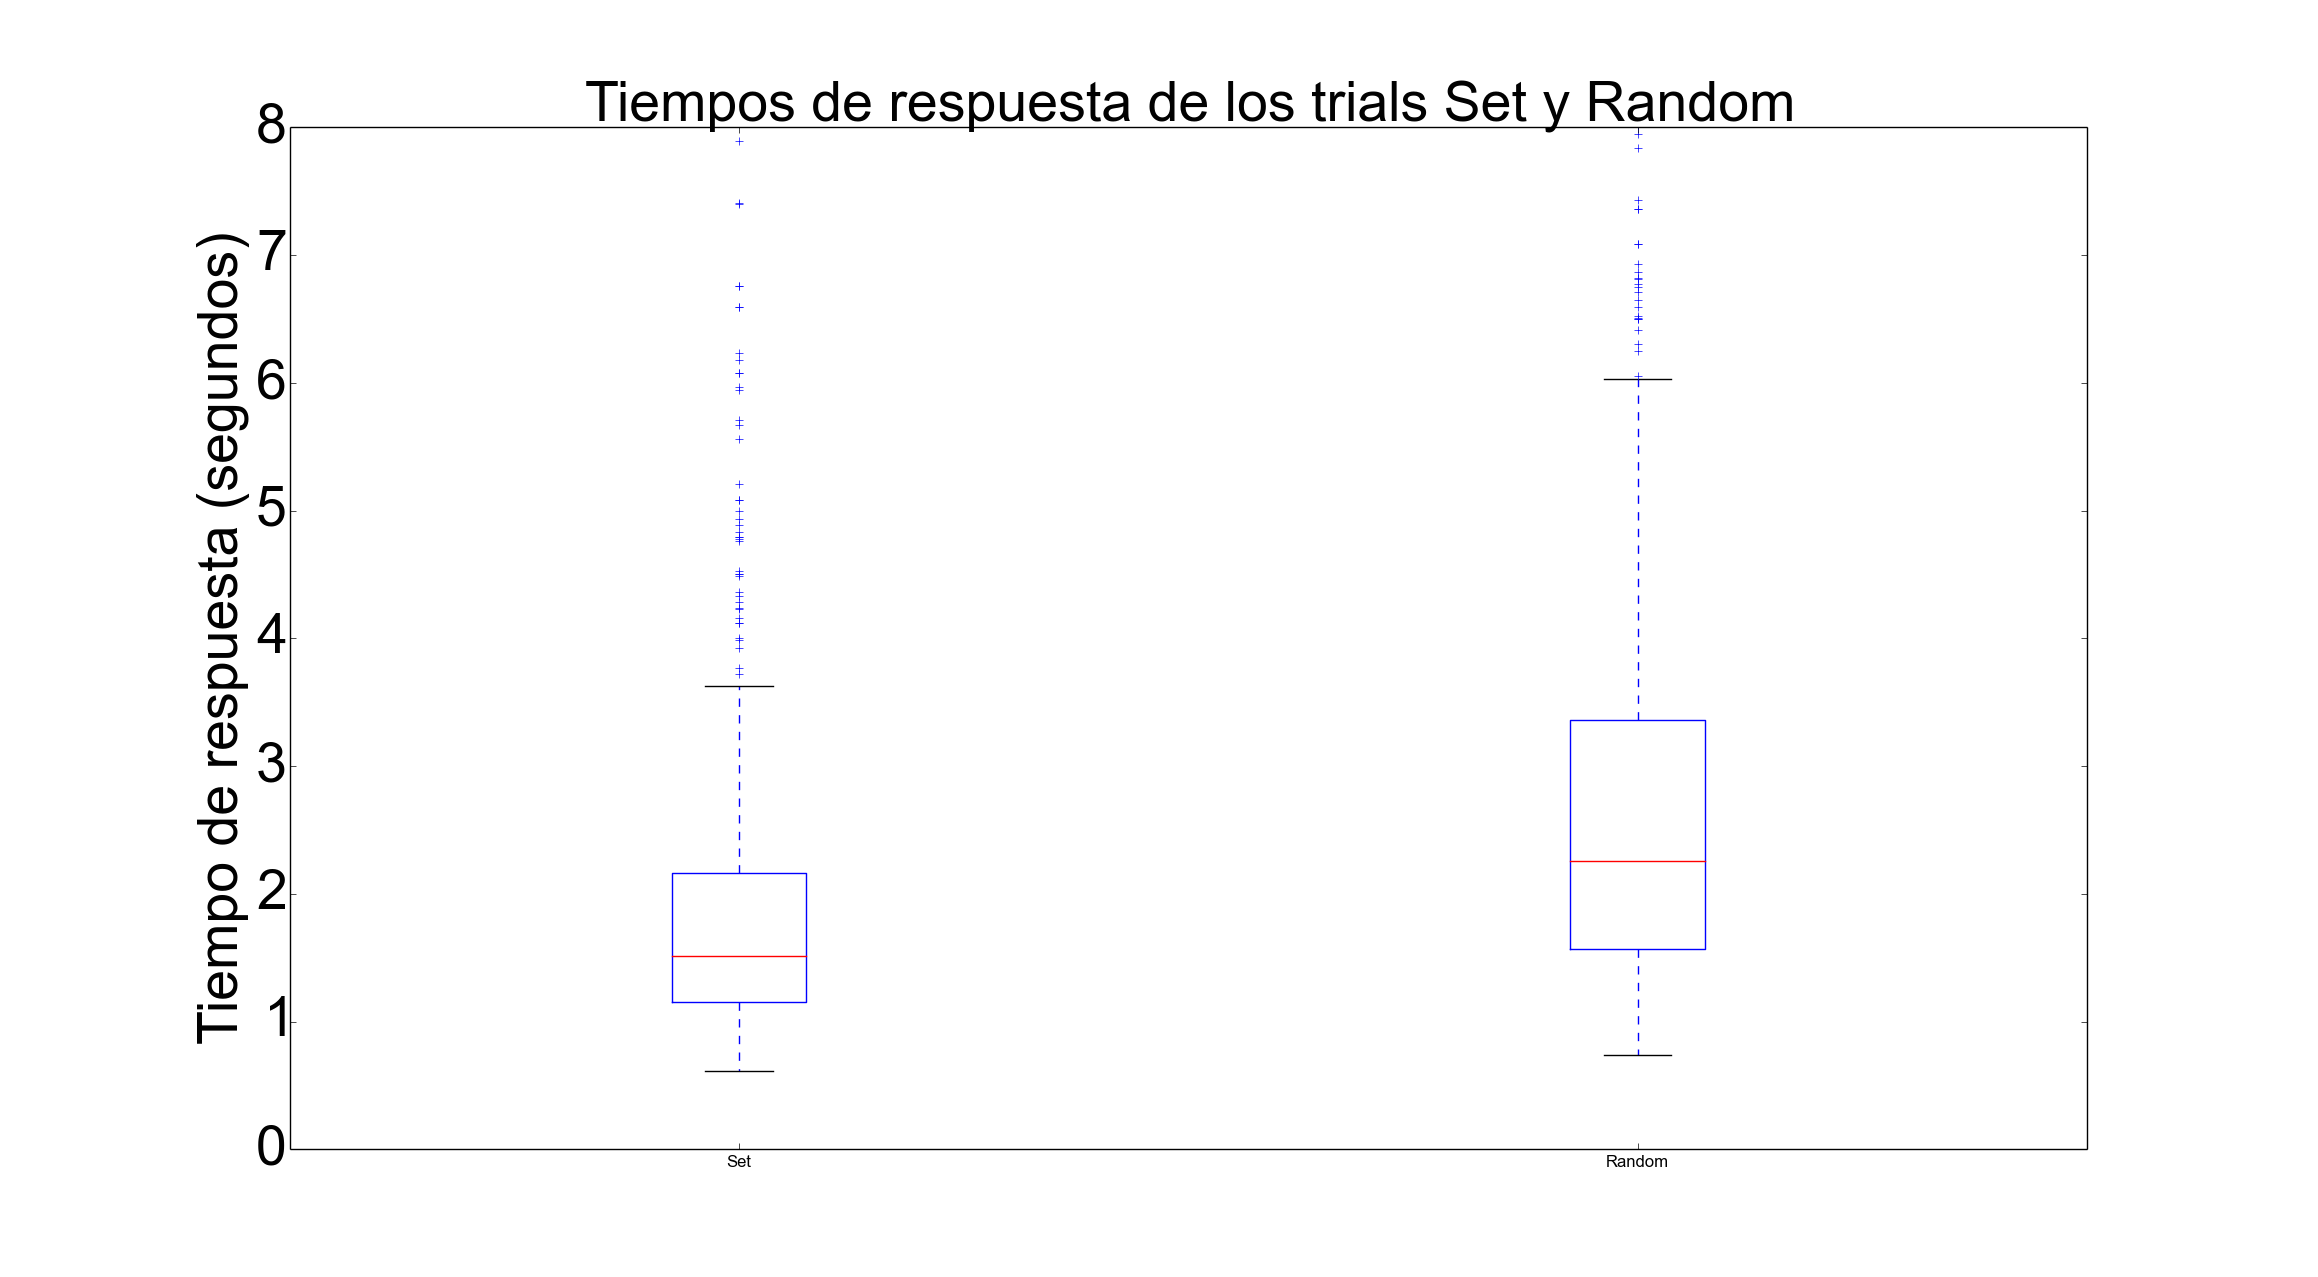
\includegraphics[scale=0.22]{rt.png}
  \end{minipage}
\end{figure}
\end{frame}

\begin{frame}
\begin{figure}[c]
 \centering
  \begin{minipage}[c]{1\textwidth}
	\centering	
	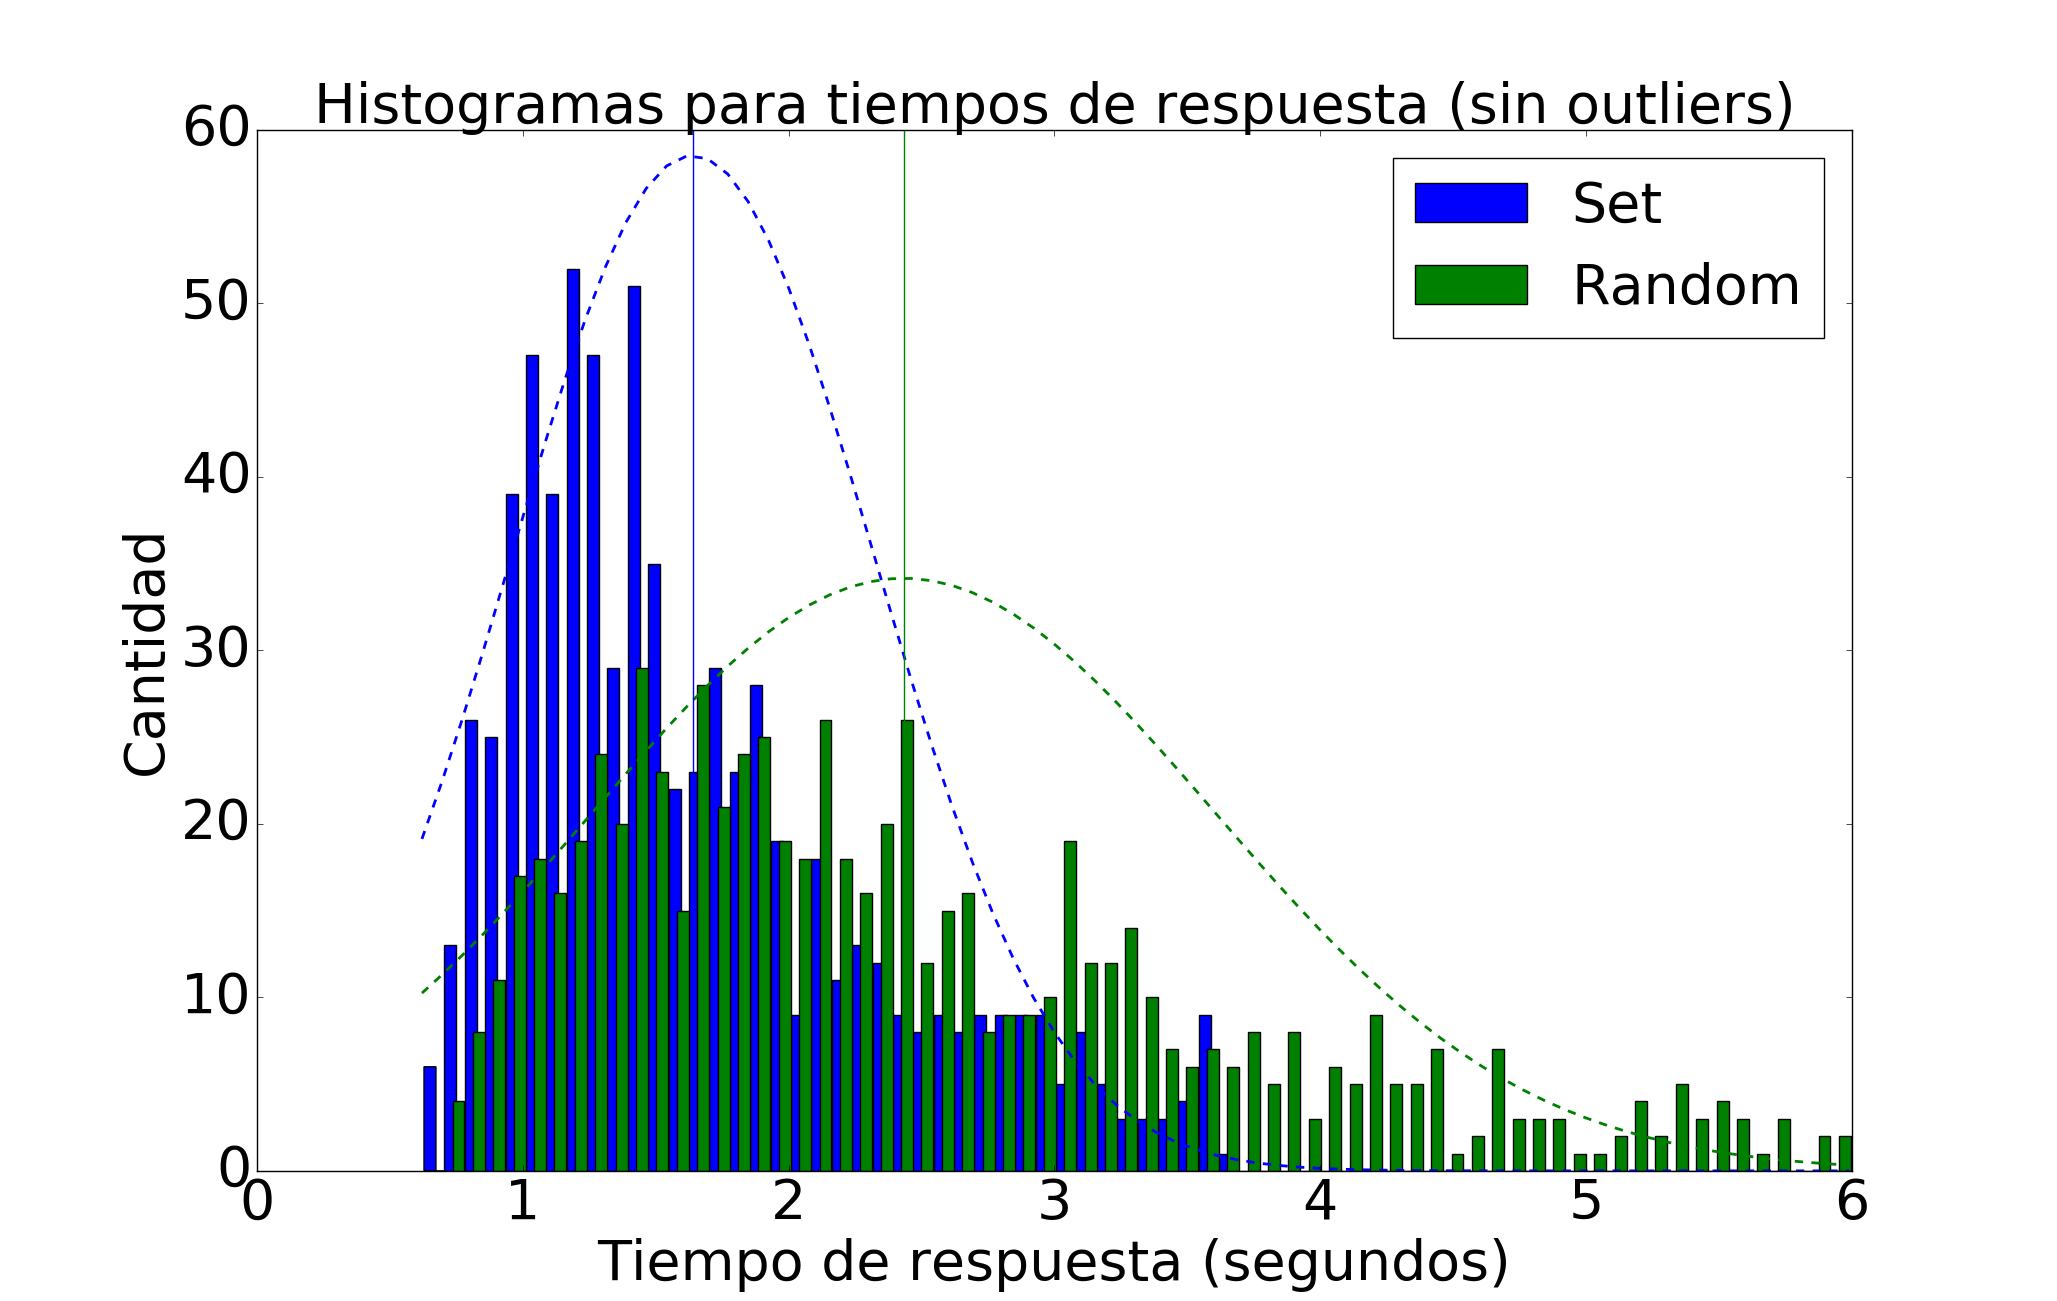
\includegraphics[scale=0.22]{rt_hist.png}
  \end{minipage}
\end{figure}
\end{frame}

\subsection{Clases}

\begin{frame}
\begin{figure}[c]
 \centering
  \begin{minipage}[c]{1\textwidth}
	\centering	
	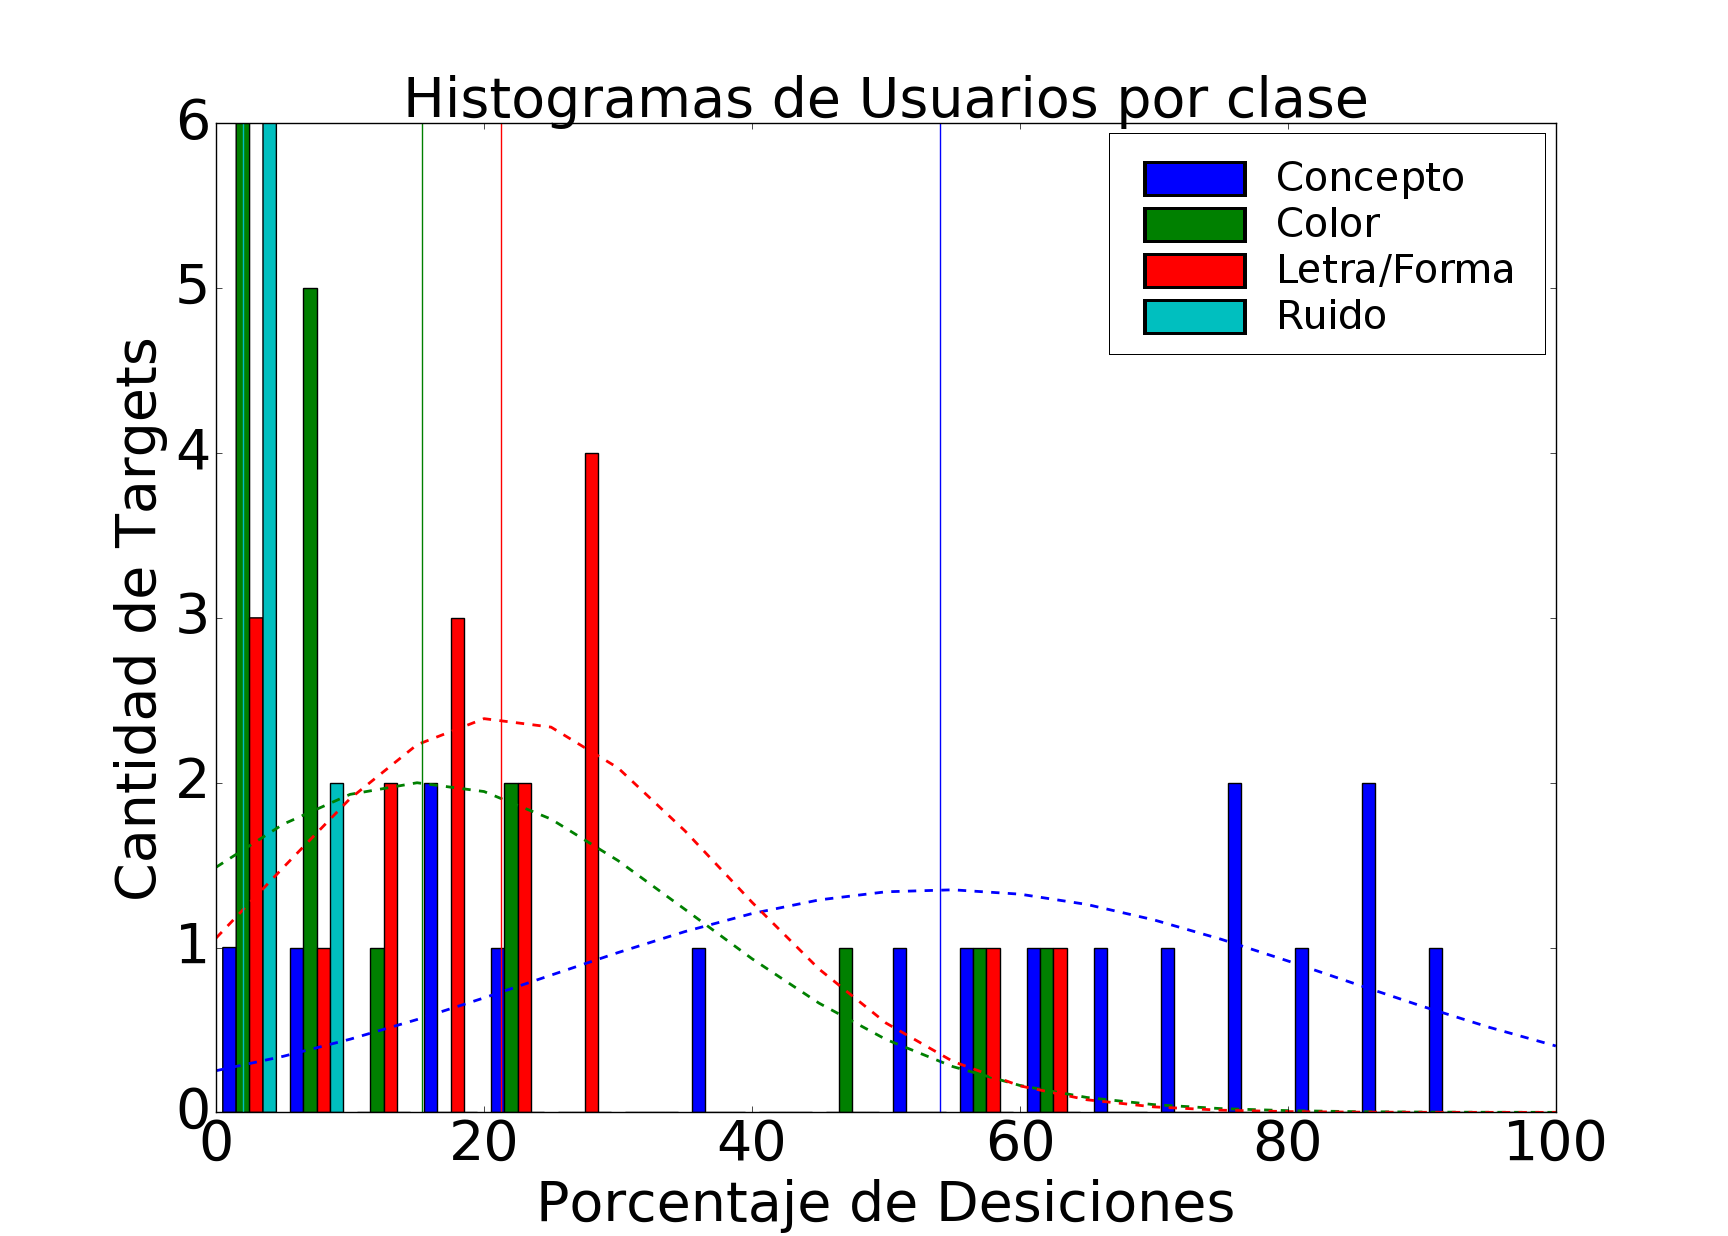
\includegraphics[scale=0.27]{hist_users.png}
  \end{minipage}
\end{figure}
\end{frame}

\begin{frame}
\begin{figure}[c]
 \centering
  \begin{minipage}[c]{1\textwidth}
	\centering	
	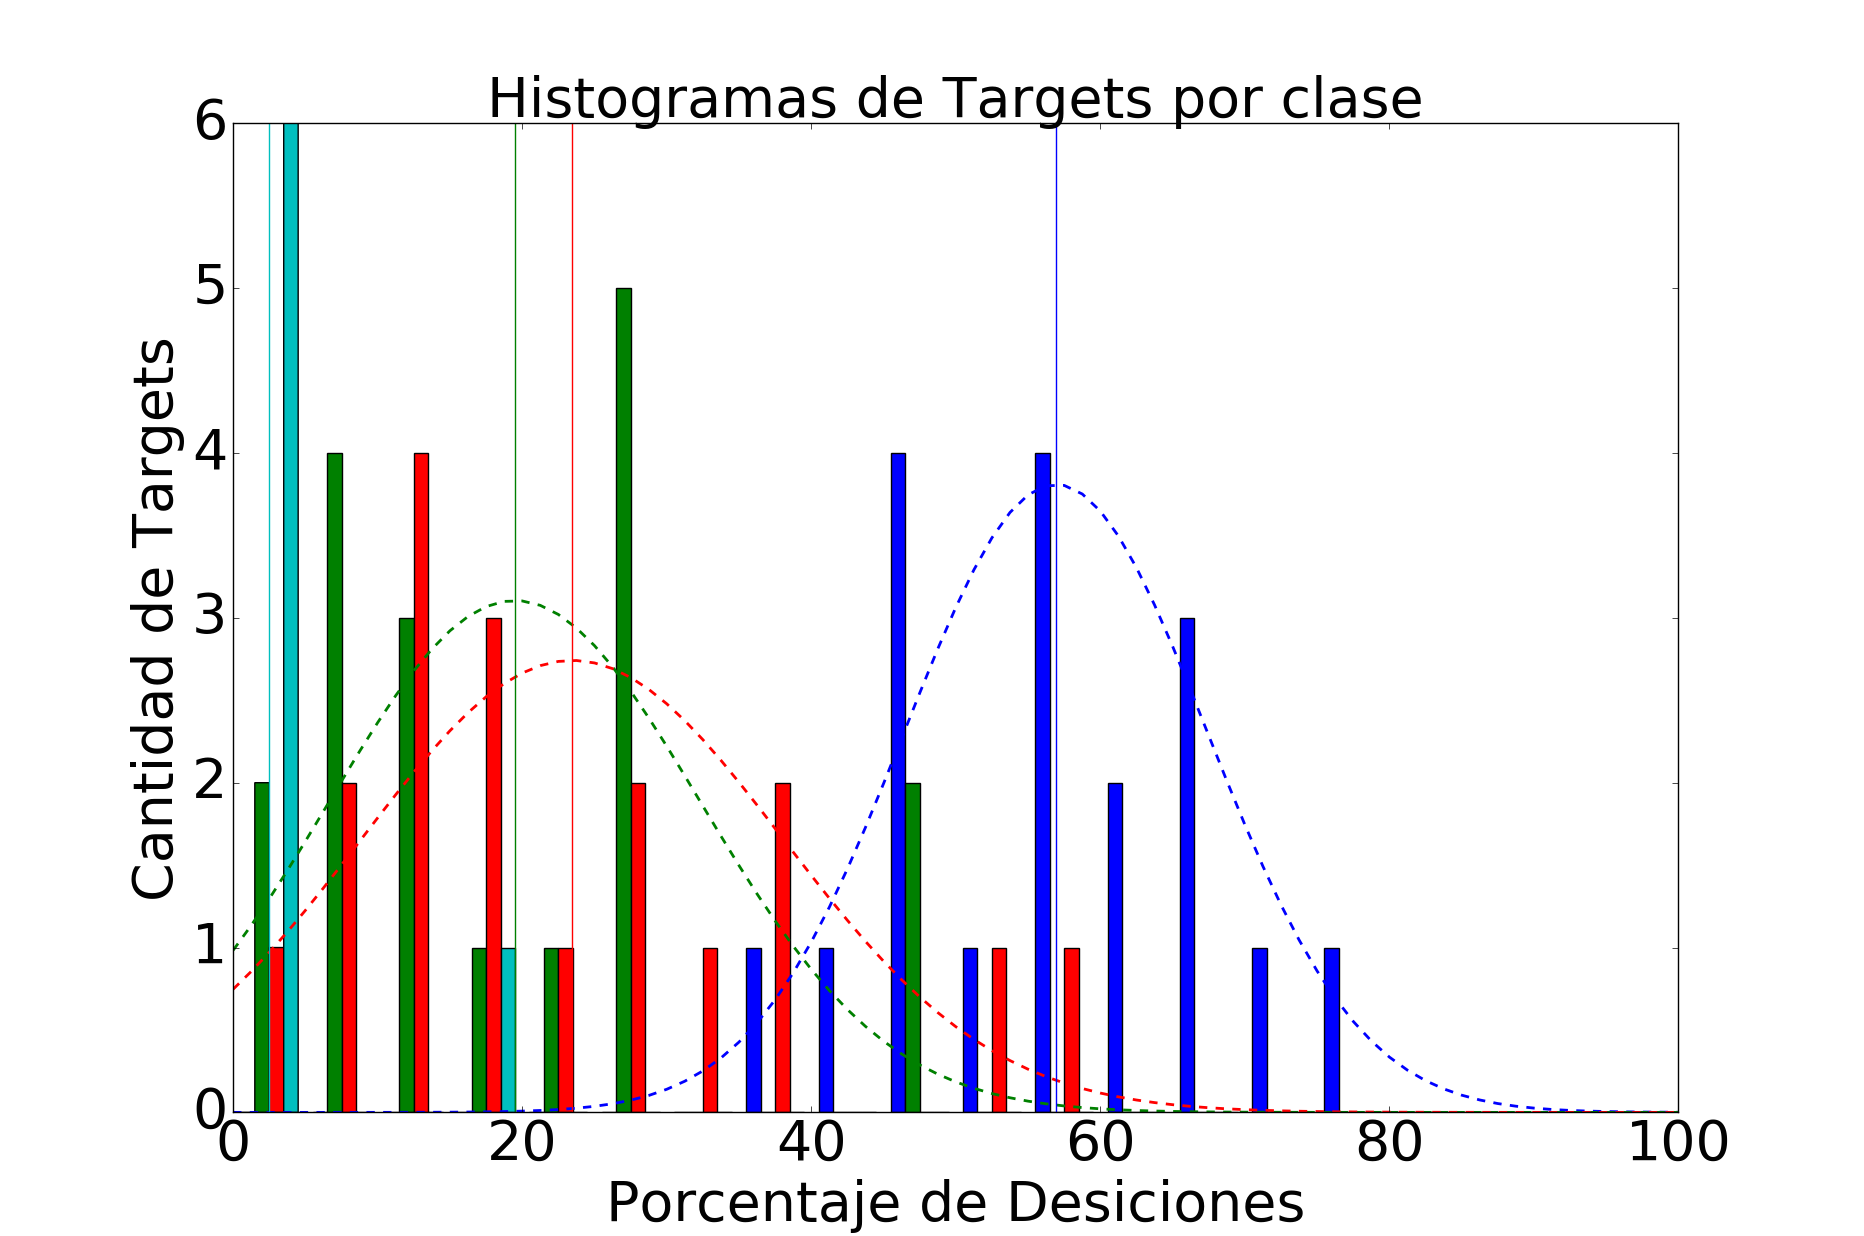
\includegraphics[scale=0.27]{hist_targets.png}
  \end{minipage}
\end{figure}
\end{frame}

\section{Tests}

\begin{frame}{Test shapiro - Normalidad}

La hipótesis nula de esta prueba es que la población tiene una distribución normal. Por lo tanto si el p-valor es menor a alfa (nivel de confianza) entonces la hipótesis nula es rechazada (se concluye que los datos no vienen de una distribución normal).

\begin{center}
    \begin{tabular}{ | p{2cm} | p{3.5cm} | p{2cm} |}
    \hline
     clase       &  p-value               & Rechaza H0		\\ 
    \hline
     Ruido       &  9.67449295786e-07     & True 				\\ 
     Color       &  0.138976812363   	  &	False				\\ 
     Letra/Forma &  0.0948526263237       & False 				\\ 
	 Concepto    &  0.733717143536   	  &	False			\\ 
    \hline
    \end{tabular}
\end{center} 

\end{frame}

\begin{frame}{Test bartlett - Homocedasticidad}

{\Large ESTA BIEN LA DESCRIPCION DE LO QUE HACE BARTLETT?}

La prueba de Bartlett se utiliza para probar la hipótesis nula, H0 que todas las varianzas de una población k son iguales, frente a la hipótesis alternativa de que al menos dos son diferentes.
Por lo tanto si el p-valor es menor a alfa (nivel de confianza) entonces la hipótesis nula es rechazada, es decir hay una diferencia signitificativa en las varianzas.

$P-value$ : 0.413846834579

\end{frame}

\begin{frame}{Test Anova - comparación de medias}

{\Large ESTA BIEN LA DESCRIPCION DE LO QUE HACE ANOVA?}
{\Large BARTLETT HACE LO MISMO QUE ANOVA TIENE SENTIDO TENER LOS DOS?}

La prueba ANOVA (Analysis Of Variance) permite comparar simultaneamente todas las medias. Como su nombre lo indica, compara varianzas aunque lo que contrastamos son medias. La hipotesis nula es que las medias no tienen diferencias significativas.
Si el p-valor es menor a alfa (nivel de confianza) entonces la hipótesis nula es rechazada, es decir hay una diferencia signitificativa en las medias.

$P-value$ : 7.03090345431e-12

\end{frame}

\begin{frame}{Test Tukey}

El Test de Tukey es un test de comparaciones múltiples. Permite comparar las medias de los t niveles de un factor después de haber rechazado la Hipótesis nula de igualdad de medias mediante la técnica ANOVA. 

Se establece así un umbral, como en otros métodos. Se calculan todas las diferencias de medias muestrales entre los t niveles del factor estudiado. 

{\Large QUE SIGNIFICA ESE REJECT, ES RECHAZAR H0 NO?}


\begin{center}
    \begin{tabular}{ | p{1.7cm} | p{1.7cm} | p{1.4cm} | p{1.4cm} | p{1.4cm} | p{0.9cm} |}
    \hline
	 \multicolumn{6}{|c|}{Multiple Comparison of Means - Tukey HSD,FWER=0.05 } \\
    \hline
     group1       &  group2      & meandiff & lower    & upper    & reject \\ 
     color        &  concepto    & 37.4293  & 26.8863   &  47.9722 & True   \\ 
     color        &  letra/forma & 3.9808   & -6.5621   &  14.5237 & False  \\ 
	 concepto     &  letra/forma & -33.4485 & -43.9914 &  -22.9056  & True  \\ 
    \hline
    \end{tabular}
\end{center} 

\end{frame}


\begin{frame}{T-Test}

Se trata de una prueba bilateral para la hipótesis nula de que 2 muestras independientes tienen idénticos valores madios (esperados). Esta prueba asume que las poblaciones tienen varianzas iguales.

\begin{center}
    \begin{tabular}{ | p{2cm} | p{2cm} | p{3.5cm} | p{2cm} |}
    \hline
     Clase1       &  Clase2 			&  p-value               & Rechaza H0		\\ 
    \hline
     Concepto    &  Letra/Forma	    &  6.04027331118e-09     & True 				\\ 
     Concepto    &  Color 			&  7.02800170074e-11   	 & True				\\ 
     Color 		 &  Letra/Forma     &  0.40368990303         & False 				\\ 
    \hline
    \end{tabular}
\end{center} 

\end{frame}





%\begin{center}
%    \begin{tabular}{ | p{1.7cm} | p{1.7cm} | p{1.4cm} | p{1.4cm} | p{1.4cm} | p{0.9cm} |}
%    \hline
%	 \multicolumn{6}{|c|}{Multiple Comparison of Means - Tukey HSD,FWER=0.05 } \\
 %   \hline
%     group1       &  group2      & meandiff & lower    & upper    & reject \\ 
%     color        &  concepto    & 17.8125  & 7.6811   &  27.9439 & True   \\ 
%     color        &  letra/forma & 2.0      & -8.1314  &  12.1314 & False  \\ 
%     color        &  ruido       & -8.0     & -18.1314 &  2.1314  & False  \\ 
%	 concepto     &  letra/forma & -15.8125 & -25.9439 & -5.6811  & True  \\ 
%     concepto     &  ruido       & -25.8125 & -35.9439 & -15.6811 & True   \\ 
%     letra/forma  &  ruido       & -10.0    & -20.1314 & 0.1314   & False  \\ 
%    \end{tabular}
%\end{center} 


%\begin{center}
%    \begin{tabular}{ | p{1.7cm} | p{1.7cm} | p{1.4cm} | p{1.4cm} | p{1.4cm} | p{0.9cm} |}
%    \hline
%	 \multicolumn{6}{|c|}{Multiple Comparison of Means - Tukey HSD,FWER=0.05 } \\
%    \hline
%     group1       &  group2      & meandiff & lower    & upper    & reject \\ 
%     color        &  concepto    &  0.2077  & 0.0706   & 0.3447   & True  \\ 
%     color        &  letra/forma &  0.0198  & -0.1173  & 0.1569   & False \\ 
%     color        &  ruido       &  -0.1207 & -0.2578  & 0.0164   & False \\ 
%	 concepto     &  letra/forma &  -0.1879 & -0.3249  & -0.0508  & True \\ 
%     concepto     &  ruido       &  -0.3283 & -0.4654  & -0.1912  & True  \\ 
%     letra/forma  &  ruido       &  -0.1405 & -0.2776  & -0.0034  & True \\ 
%    \end{tabular}
%\end{center} 


                   
%['color' 'concepto' 'letra/forma' 'ruido']


%Anova Cantidad de elecciones de un usuario por clase 1.02032498869e-07 \\
%Anova Cantidad de elecciones de un usuario por clase / cantidad de jugadas del usuario 6.60708232706e-07 \\


% Placing a * after \section means it will not show in the
% outline or table of contents.
\section*{Summary}

\begin{frame}{Summary}
  \begin{itemize}
  \item
    The \alert{first main message} of your talk in one or two lines.
  \item
    The \alert{second main message} of your talk in one or two lines.
  \item
    Perhaps a \alert{third message}, but not more than that.
  \end{itemize}
  
  \begin{itemize}
  \item
    Outlook
    \begin{itemize}
    \item
      Something you haven't solved.
    \item
      Something else you haven't solved.
    \end{itemize}
  \end{itemize}
\end{frame}

\begin{frame}
\begin{figure}[h]
 \centering
  \begin{minipage}[c]{1\textwidth}
	\centering	
	
\includegraphics[scale=0.4]{bender.jpg}
  \end{minipage}
\end{figure}
\end{frame}

% All of the following is optional and typically not needed. 
\appendix
\section<presentation>*{\appendixname}
\subsection<presentation>*{For Further Reading}

\begin{frame}[allowframebreaks]
  \frametitle<presentation>{For Further Reading}
    
  \begin{thebibliography}{10}
    
  \beamertemplatebookbibitems
  % Start with overview books.

  \bibitem{Author1990}
    A.~Author.
    \newblock {\em Handbook of Everything}.
    \newblock Some Press, 1990.
 
    
  \beamertemplatearticlebibitems
  % Followed by interesting articles. Keep the list short. 

  \bibitem{Someone2000}
    S.~Someone.
    \newblock On this and that.
    \newblock {\em Journal of This and That}, 2(1):50--100,
    2000.
  \end{thebibliography}
\end{frame}

\end{document}


